\documentclass[12pt,twoside,openright]{report}
\usepackage[utf8]{inputenc}
\usepackage[T1]{fontenc}
\usepackage[english]{babel}
\usepackage[a4paper,width=150mm,top=25mm,bottom=25mm]{geometry}

% paragraph
\setlength{\parindent}{0em}
\setlength{\parskip}{1em}

% headers and footers
\usepackage{fancyhdr}
\pagestyle{fancy}
% common
\fancyhead{}
\fancyhead[RO,LE]{\leftmark}
\fancyfoot{}
\fancyfoot[LE,RO]{\thepage}
\renewcommand{\headrulewidth}{0.4pt}
\renewcommand{\footrulewidth}{0.4pt}
% layouts, chapters, etc.
\fancypagestyle{plain}{%
    \fancyhead{}
    \fancyfoot{}
    \fancyfoot[LE,RO]{\thepage}
    \renewcommand{\headrulewidth}{0pt}
    \renewcommand{\footrulewidth}{0.4pt}
}

% blank pages
\makeatletter
\def\cleardoublepage{\clearpage\if@twoside \ifodd\c@page\else
    \hbox{}
    \thispagestyle{empty}
    \newpage
    \if@twocolumn\hbox{}\newpage\fi\fi\fi}
\makeatother

% images
\usepackage{graphicx}
\graphicspath{ {images/} }
\usepackage{array}
\usepackage{caption}
\usepackage{subcaption}

% tables
\setlength{\arrayrulewidth}{0.5mm}
\setlength{\tabcolsep}{18pt}
\renewcommand{\arraystretch}{1.5}
\newcolumntype{M}[1]{>{\centering\arraybackslash}m{#1}}

% equations
\usepackage{amsmath}

% algorithms
% \usepackage{amsmath}
\usepackage{algorithm}
\usepackage{algpseudocode}
% \newcommand\CONDITION[2]%
%   {\begin{tabular}[t]{@{}l@{}l@{}}
%      #1&#2
%    \end{tabular}%
%   }
% \algdef{SE}[WHILE]{While}{EndWhile}[1]%
%     {\algorithmicwhile\ \CONDITION{#1}{\ \algorithmicdo}}%
%     {\algorithmicend\ \algorithmicwhile}
% \algdef{SE}[FOR]{For}{EndFor}[1]%
%     {\algorithmicfor\ \CONDITION{#1}{\ \algorithmicdo}}%
%     {\algorithmicend\ \algorithmicfor}
% \algdef{S}[FOR]{ForAll}[1]%
%     {\algorithmicforall\ \CONDITION{#1}{\ \algorithmicdo}}
% \algdef{SE}[REPEAT]{Repeat}{Until}{\algorithmicrepeat}[1]%
%     {\algorithmicuntil\ \CONDITION{#1}{}}
% \algdef{SE}[IF]{If}{EndIf}[1]%
%     {\algorithmicif\ \CONDITION{#1}{\ \algorithmicthen}}%
%     {\algorithmicend\ \algorithmicif}%
% \algdef{C}[IF]{IF}{ElsIf}[1]%
%     {\algorithmicelse\ \algorithmicif\ \CONDITION{#1}{\ \algorithmicthen}}

% code
\usepackage{listings}
\lstdefinelanguage{JavaScript}{
    keywords={typeof, new, true, false, catch, function, return, null, catch, switch, var, if, in, while, do, else, case, break},
    keywordstyle=\color{blue}\bfseries,
    ndkeywords={class, export, boolean, throw, implements, import, this},
    ndkeywordstyle=\color{darkgray}\bfseries,
    identifierstyle=\color{black},
    sensitive=false,
    comment=[l]{//},
    morecomment=[s]{/*}{*/},
    commentstyle=\color{purple}\ttfamily,
    stringstyle=\color{red}\ttfamily,
    morestring=[b]',
    morestring=[b]"
}
\lstset{
    language=JavaScript,
    backgroundcolor=\color{lightgray},
    extendedchars=true,
    basicstyle=\footnotesize\ttfamily,
    showstringspaces=false,
    showspaces=false,
    numbers=left,
    numberstyle=\footnotesize,
    numbersep=9pt,
    tabsize=2,
    breaklines=true,
    showtabs=false,
    captionpos=b
}

% bibliography
\usepackage[nottoc]{tocbibind}

% hyperlinks
\usepackage{hyperref}
\hypersetup{
    colorlinks=true,
    linkcolor=black,
    urlcolor=black,
    citecolor=black,
}

\begin{document}

\pagenumbering{gobble}
\begin{titlepage}
    \begin{center}
        \vspace*{1cm}
        
        \huge
        \textbf{Visualization of Internal Blockchain Processes}
        
        \vspace{2cm}
        
        \large
        Shao-Chun Ma \\
        \href{mailto:shao-chun.ma@rwth-aachen.de}{shao-chun.ma@rwth-aachen.de} \\
        Matriculation number: 373895

        \vspace{1cm}

        Supervisor: Prof. Dr. Thomas Rose \\
        Advisor: Thomas Osterland \\

        \vspace{1.5cm}

        Chair for Computer Science 5 \\
        Information Systems \\
        RWTH Aachen
        
        \vfill
        
        This thesis is submmited for the degree of \\
        M.Sc. Software Systems Engineering
        
        \vspace{3cm}
        
        Aachen, Germany \\
        May 2018
        
    \end{center}
\end{titlepage}
\cleardoublepage

\pagenumbering{roman}
\thispagestyle{plain}
\topskip0pt
\vspace*{\fill}
    \begin{center}
        \Large
        \textbf{Abstract}
    \end{center}
    
    \vspace{1cm}
    
    In a blockchain system, many nodes spread transactions and blocks simultaneously. Therefore, the behaviors of nodes and the mining processes are complex and difficult to identify. In this paper, we present a visualization tool which identifies the influences of the network delay and the mining strategies of miners on mining processes in a blockchain system which employs proof-of-work as the consensus protocol. Our approach is based on the simulation of a blockchain system, which is built on a platform of the multi-agent system. The data sent between the nodes are monitored and recorded by the watchdog, and then they are sent to the visualizer. As a result, the visualizer can provide a fantastic visualization of internal blockchain processes in real-time. We provide scenarios to demonstrate the potential applications of the visualization tool. Consequently, it proves that the visualization tool is suitable for helping researchers to analyze the mining processes clearly and correctly. \\
    
    \textbf{Keywords}: \textit{blockchain; visualization; mining strategy; network delay; proof-of-work}
\vspace*{\fill}


\cleardoublepage

\thispagestyle{plain}
\topskip0pt
\vspace*{\fill}
    \begin{center}
        \Large
        \textbf{Declaration}
    \end{center}

    \vspace{1cm}

    fff
\vspace*{\fill}

\cleardoublepage

\thispagestyle{plain}
\topskip0pt
\vspace*{\fill}
    \begin{center}
        \Large
        \textbf{Acknowledgements}
    \end{center}

    \vspace{1cm}

    First, I would like to appreciate the useful guides and suggestions from the supervisor, Prof. Dr. Thomas Rose, and the advisor, Thomas Osterland. Additionally, Prof. Wolfgang Prinz also helped me to improve the weakness of this thesis. Last but not the least, I owe the success of this thesis to my parents, Li-Ju Chen and Yuan-Chun Ma, and my wife, Yu-Ming Chien. They supported me through the difficulties that I encountered during the work.
\vspace*{\fill}

\cleardoublepage

\tableofcontents

\listoffigures
 
\listoftables

\listofalgorithms

\chapter{Introduction}
\pagenumbering{arabic}
The blockchain technology was first proposed in Satoshi Nakamoto’s paper, \textit{Bitcoin: A Peer-to-Peer Electronic Cash System} \cite{Nakamoto2008}, in 2008. It created a new type of digital currency, called \textit{cryptocurrency}. For example, Bitcoin \cite{bitcoin} and Ethereum \cite{ethereum} are two of the well-known cryptocurrencies. Cryptocurrencies have a significant characteristic that distinguishes them from traditional currencies: they are decentralized. This means that there is no authority in cryptocurrencies. The single authority in conventional currencies is necessary as it prevents the problem of double-spending. Therefore, the validity of transactions are important in cryptocurrencies, and it is fulfilled by consensus protocols which are based on cryptography techniques. \cite{Narayanan2016}

The major process of the blockchain systems starts with the creation of a transaction. This transaction is distributed over the blockchain network. In this state, the transaction is not-mined and therefore not persistent. Every node in the network has its own transaction pools that contain the not-mined transactions.

In a blockchain system with the proof-of-work protocol, the nodes maintain the blockchain data structure by themselves. They compete against each other in extending the blockchain by creating new blocks that persistently store transactions from the transaction pools. The addition of new blocks provides effort, since it is necessary to solve a cryptographic puzzle with the characteristic that it is hard to solve, but easy to verify given a correct solution. The solving process is called mining. A correct solution is distributed over the network and verified by the remaining network participants. In the case that the verification succeeds, the block is added to the blockchain, and the containing transactions are removed from the transaction pools.

\section{Motivation}

There are two factors that play important roles in the mining processes: the \textit{network delay} and the different \textit{mining strategies} of miners. While a transaction is published through the blockchain network, each node receives it at a different time due to characteristics of peer-to-peer networks. Therefore, each miner has different pending transactions in the transaction pool at the same time. Moreover, each miner mines a block according to the individual mining strategy simultaneously. The blocks generated by miners are different from each other, and they are also published through the unstable peer-to-peer network. Consequently, it is possible that the set of nodes partitions into different groups that work on different instances of the blockchain. These blockchains are maintained simultaneously until one blockchain becomes longer. The longest blockchain in the network is assumed to be the correct one, which is resolved by the consensus protocol.

\begin{figure}[htb]
    \centering
    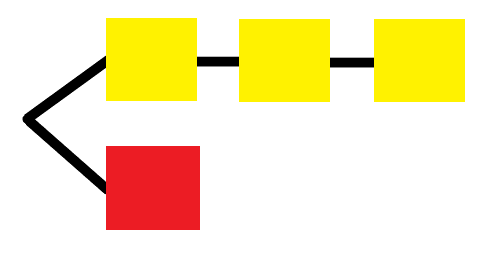
\includegraphics[width=0.7\textwidth]{intro_longest}
    \caption{Red blocks are considered to be the longest blockchain.}
    \label{fig:red blocks are considered to be the longest blockchain}
\end{figure}

For a simple example, the red blocks are the longest blockchain in Figure \ref{fig:red blocks are considered to be the longest blockchain}. There are forks on the path because of the past competitions.

In a real blockchain system, for example, there are about ten thousand of nodes in Bitcoin in April 2018 from an online statistical result \footnote{\url{https://bitnodes.earn.com/}}. For such wide and massive blockchain networks, it is hard to analyze the individual behavior of each node, e.g., the influences of the mining strategy to the mining processes under the unstable peer-to-peer network. Moreover, the mining processes of a blockchain system described earlier are dynamic and complex. Therefore, to focus on the research of the mining processes in a blockchain system, we decide to provide a visualization application to display the influences of the network delay and the mining strategy on the mining processes step by step.

\section{Methodology}

Figure \ref{fig:the method} explains the basic idea of the solution. The \textit{simulation} of the blockchain system is based on a multi-agent system, and the \textit{watchdog} monitors and records the mining activities in the blockchain system. Thus, when the transactions and the blocks are published and received by the nodes, the watchdog sends the required data to the \textit{visualizer}, which is responsible for visualizing all the mining events that happened in the blockchain system. 

\begin{figure}[htb]
    \centering
    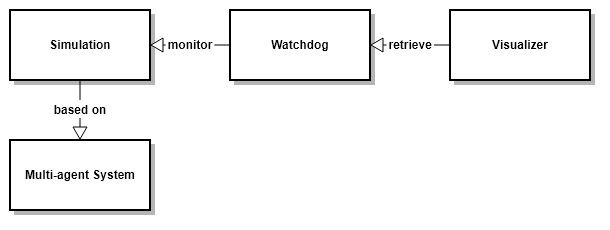
\includegraphics[width=0.8\textwidth]{intro_method}
    \caption{The method.}
    \label{fig:the method}
\end{figure}

The application is able to visualize the steps of the mining processes of each node in real-time. By setting the parameters of the network delay and the mining strategy, researchers can analyze and observe the mining processes with predefined conditions in the blockchain system. Additionally, in order to replay the same result of the blockchain processes, it is possible to provide a configuration file that defines all the properties of nodes and the parameters of the network delay and the mining strategy in the blockchain system.

\section{Contribution}

There are 8 online visualization applications, Bitbonkers, Bitnodes, BitcoinCity, Blockseer, DailyBlockchain, Elliptic, Interaqt, and Live Globe, that are summarized by Tri A. Sundara et al. \cite{Sundara2017}. Additionally, two applications, Blockchain and Etherscan, use tabular methods to represent transactions and blocks. However, these visualization applications only display the static information on Bitcoin network such as the values and the timestamps, and thus they cannot satisfy the goal which helps users to understand the dynamic mining processes. 

There are collections of previous literature that provide visualization tools to analyze the patterns of transactions on Bitcoin network. These visualization tools \cite{Kuzuno2017, Saublet2015, Fleder2015, Baumann2014} use statistical methods such as line charts, bar charts, and graph analysis to visualize the relationships and patterns of transactions and blocks. The big data visualization methods are applied \cite{McGinn2016} to find patterns of blocks. The flows of bitcoins can be tracked in the time series analysis \cite{Battista2015}. The real identification of an address can also be tracked in the analysis \cite{Kuzuno2017}. These visualization tools are implemented for analysis, though our solution focuses on visualizing the actual mining processes. 
 
Amitai Porat et al. \cite{Porat} proposed a method to analyze the potential applications of proof-of-work based blockchain networks. They considered the influences of network latency to the blockchain system. Nevertheless, our solution also considered the influences of mining strategy which are not presented in their work.

Comparing to other visualization applications and tools for blockchain systems, our solution provides the visualization of the dynamic mining processes. Furthermore, the mining processes are visualized step by step while the miners are publishing blocks through the network. Consequently, our solution is suitable for researching and understanding the complex mining processes with the factors of network delay and mining strategy.

\section{Thesis Structure}

This thesis is composed of the following chapters.

\begin{itemize}
    \item \textbf{Chapter 2} \\
        The review of the previous literature and the contribution of our approach are provided in this chapter.
    \item \textbf{Chapter 3} \\
        The assumptions and definitions of the blockchain system that the visualization is based on are given in this chapter.
    \item \textbf{Chapter 4} \\
        This chapter contains the architecture of the visualization application and the components that are implemented.
    \item \textbf{Chapter 5} \\
        In this chapter, the introduction to the usage of the visualization application is provided.
    \item \textbf{Chapter 6} \\
        Two scenarios that can be achieved by the visualization application are proposed in this chapter.
    \item \textbf{Chapter 7} \\
        At the end of this thesis, the conclusion and the future work are discussed.
\end{itemize}


\chapter{Related Works}
Since blockchain technology is proposed, different methods are experimented for visualization. As Bitcoin is the first and main blockchain network in the world and the data can be accessed publicly, much literature uses it as a research platform. Generally, there are three categories of related works for the visualization of a blockchain system.
\begin{itemize}
    \item \textbf{Visualization of Blockchains} \\
        There are a lot of online visualization tools which can visualize the static information of transactions and blocks on a blockchain system. They display the information in detail and provide it as the base for analysis.
    \item \textbf{Analysis of Transactions} \\
        As Bitcoin becomes a popular peer-to-peer network recently, most of the recent literature focuses on the analysis of the relationships between transactions and blocks in Bitcoin network. They try to recognize special patterns to gain ecnomic experience and prevent criminal activities.
    \item \textbf{Analysis of Consensus Protocols} \\
        An analysis of the consensus protocols on the blockchain networks is an interesting topic as it can reveal the potential applications on blockchain platforms.
\end{itemize}

\section{Visualization of Blockchains}

There are some online tools and applications that provide visualization of the static status of transactions and blocks in Bitcoin. Tri A. Sundara et al. \cite{Sundara2017} summarized 8 visualization applications and compared their visualization methods and technologies. We shortly reivew these applications here, so the main difference of our application and them can be identified clearly. The screenshots of the above works are in Figure \ref{fig:visualization of bitcoin}.

\begin{itemize}
    \item \textbf{Bitbonkers} \cite{bitbonkers} \\
        Bitbonkers rendered a live 3D animation of transactions and blocks. Balls represented transactions, and they kept dropping down to the plate from the top. On the other hand, cubics represented blocks. The sizes of balls are different according to their values.
    \item \textbf{Bitnodes} \cite{bitnodes} \\
        Bitnodes focused on the visualization of the distribution of nodes on Bitcoin network.
    \item \textbf{BitcoinCity} \cite{bitcoincity} \\
        BitcoinCity was a cute visualization of Bitcoin. It used a road to chain the blocks, and the houses with different heights on the both sides of the road represented transactions.
    \item \textbf{Blockseer} \cite{blockseer} \\
        Blockseer visualized the detailed information of accounts, transactions or blocks with tree structures. 
    \item \textbf{DailyBlockchain} \cite{dailyblockchain} \\
        DailyBlockchain  displayed the spread of dynamic and live Bitcoin network.
    \item \textbf{Elliptic} \cite{elliptic} \\
        Elliptic visualized the whole history of Bitcoin like the Big Bang of the universe. 
    \item \textbf{Interaqt} \cite{interaqt} \\
        Interaqt rendered the Bitcoin transactions as circles.
    \item \textbf{Live Globe} \cite{liveglobe} \\
        Live Globe combined the geographies of blocks and the earth together in the visualization.
\end{itemize}

\begin{figure}[htb]
    \centering
    \begin{subfigure}[b]{0.45\textwidth}
        \centering
        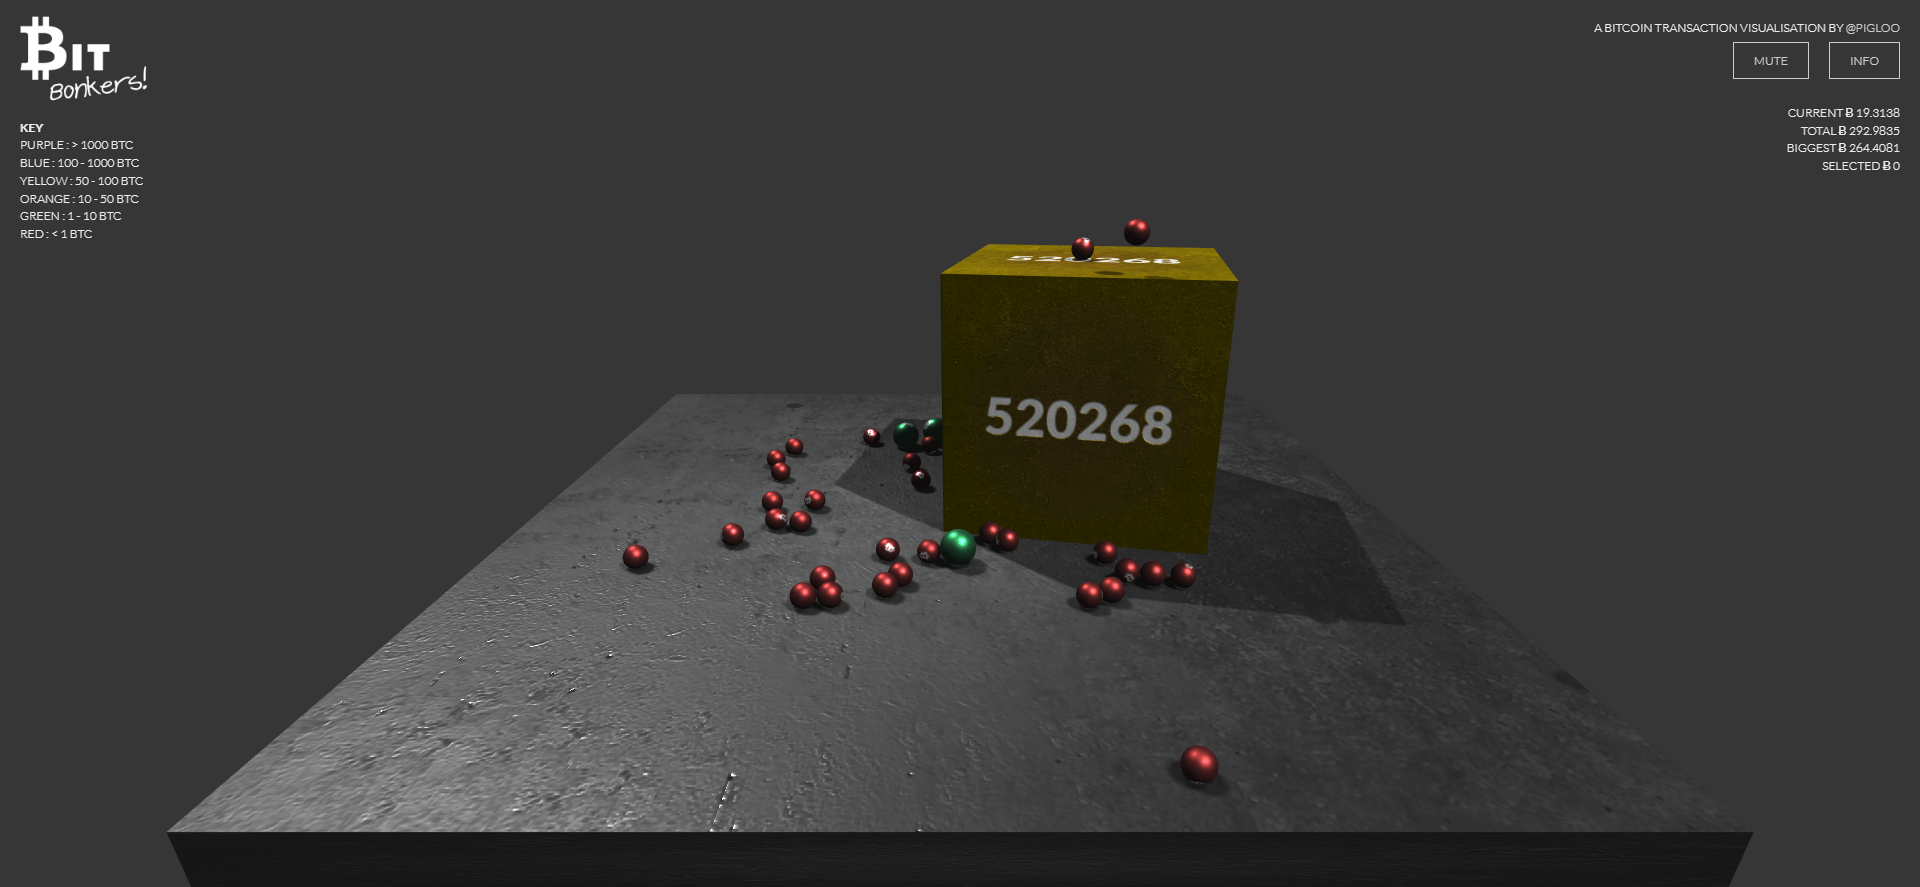
\includegraphics[width=\textwidth]{related_bitbonkers}
        \caption{Bitbonkers}
    \end{subfigure}
    \hfill
    \begin{subfigure}[b]{0.45\textwidth}
        \centering
        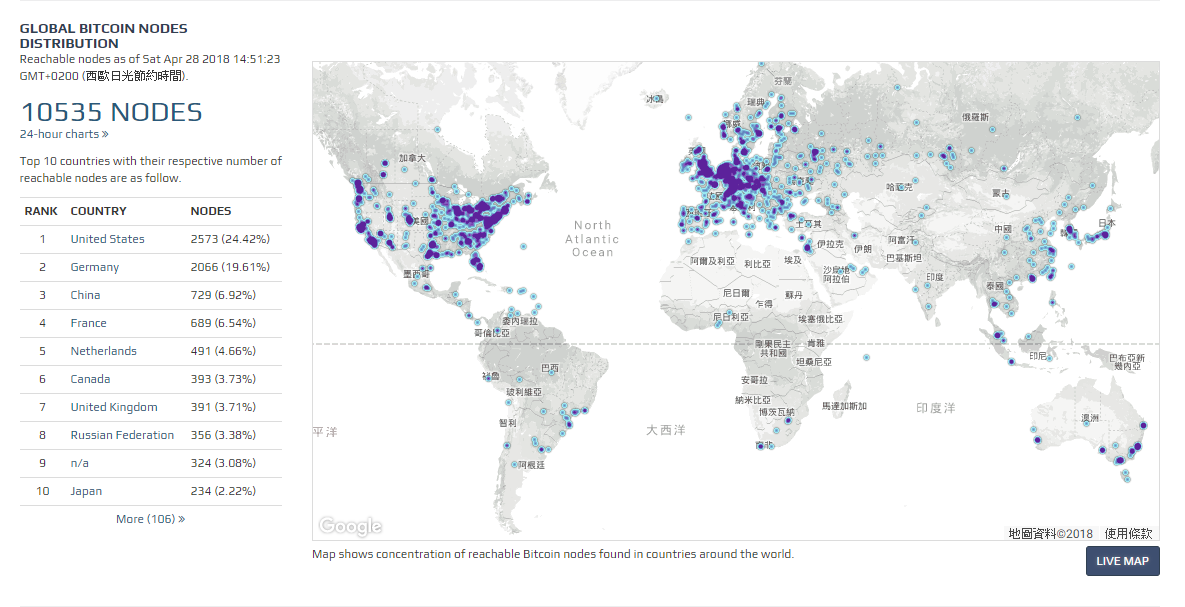
\includegraphics[width=\textwidth]{related_bitnodes}
        \caption{Bitnodes}
    \end{subfigure}

    \begin{subfigure}[b]{0.45\textwidth}
        \centering
        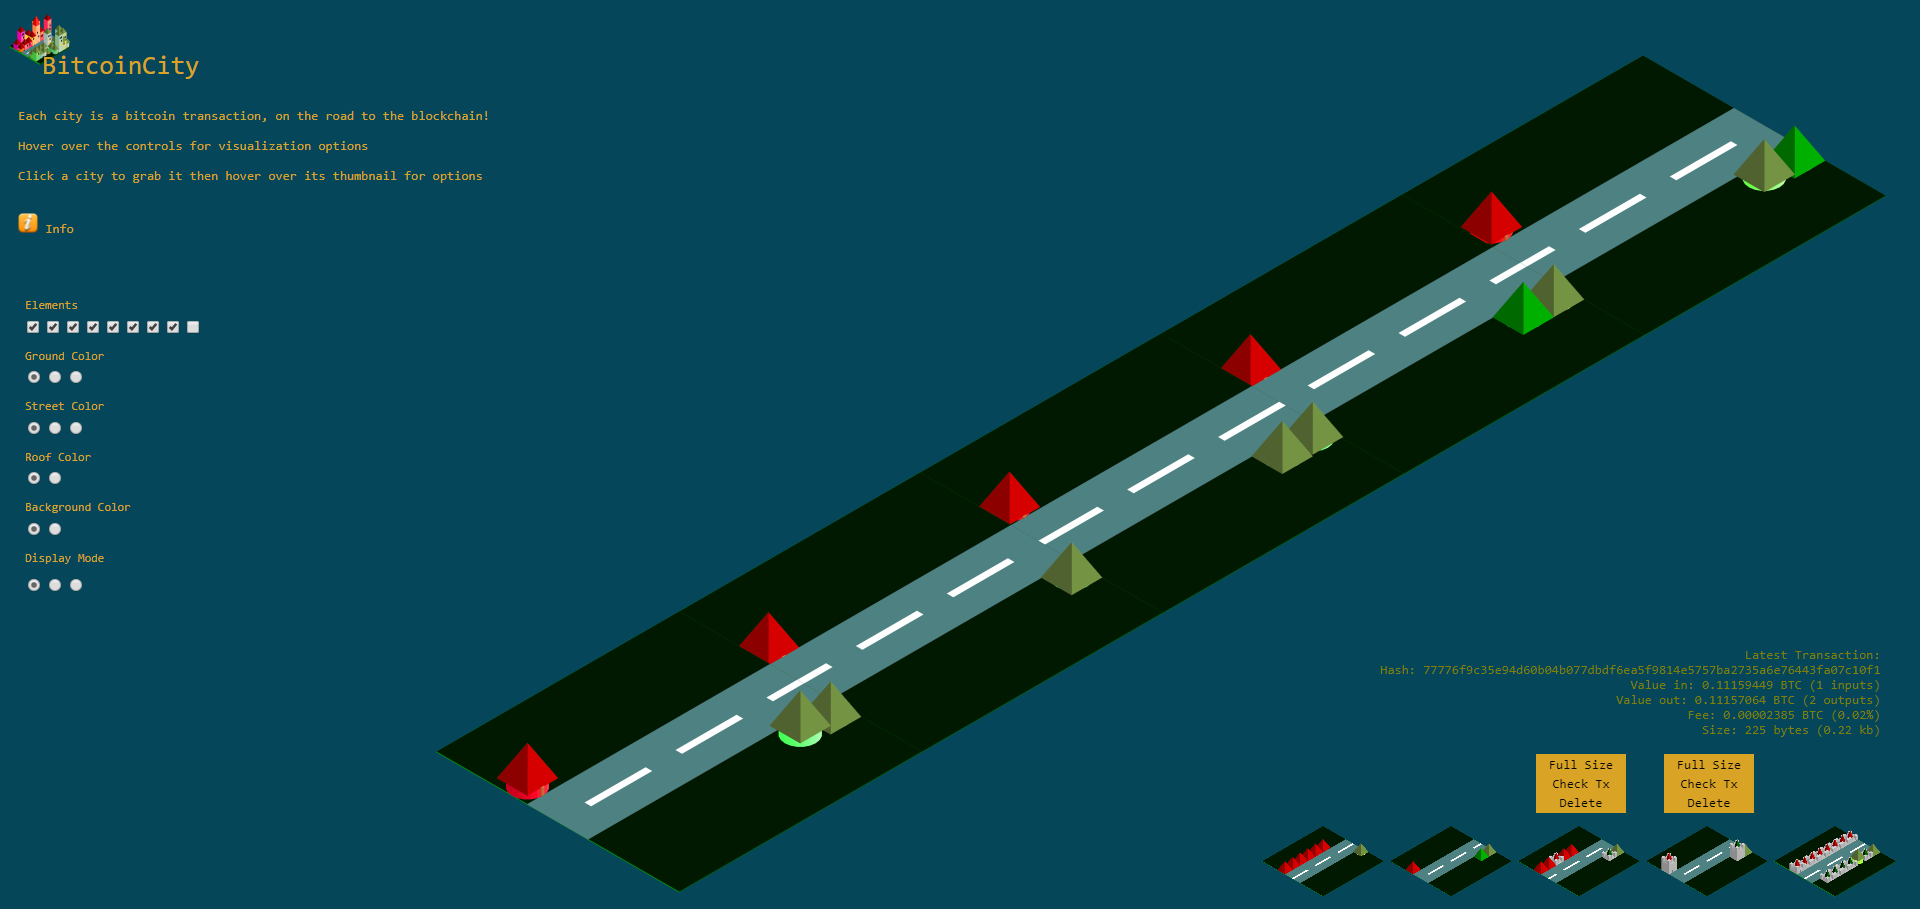
\includegraphics[width=\textwidth]{related_bitcoincity}
        \caption{BitcoinCity}
    \end{subfigure}
    \hfill
    \begin{subfigure}[b]{0.45\textwidth}
        \centering
        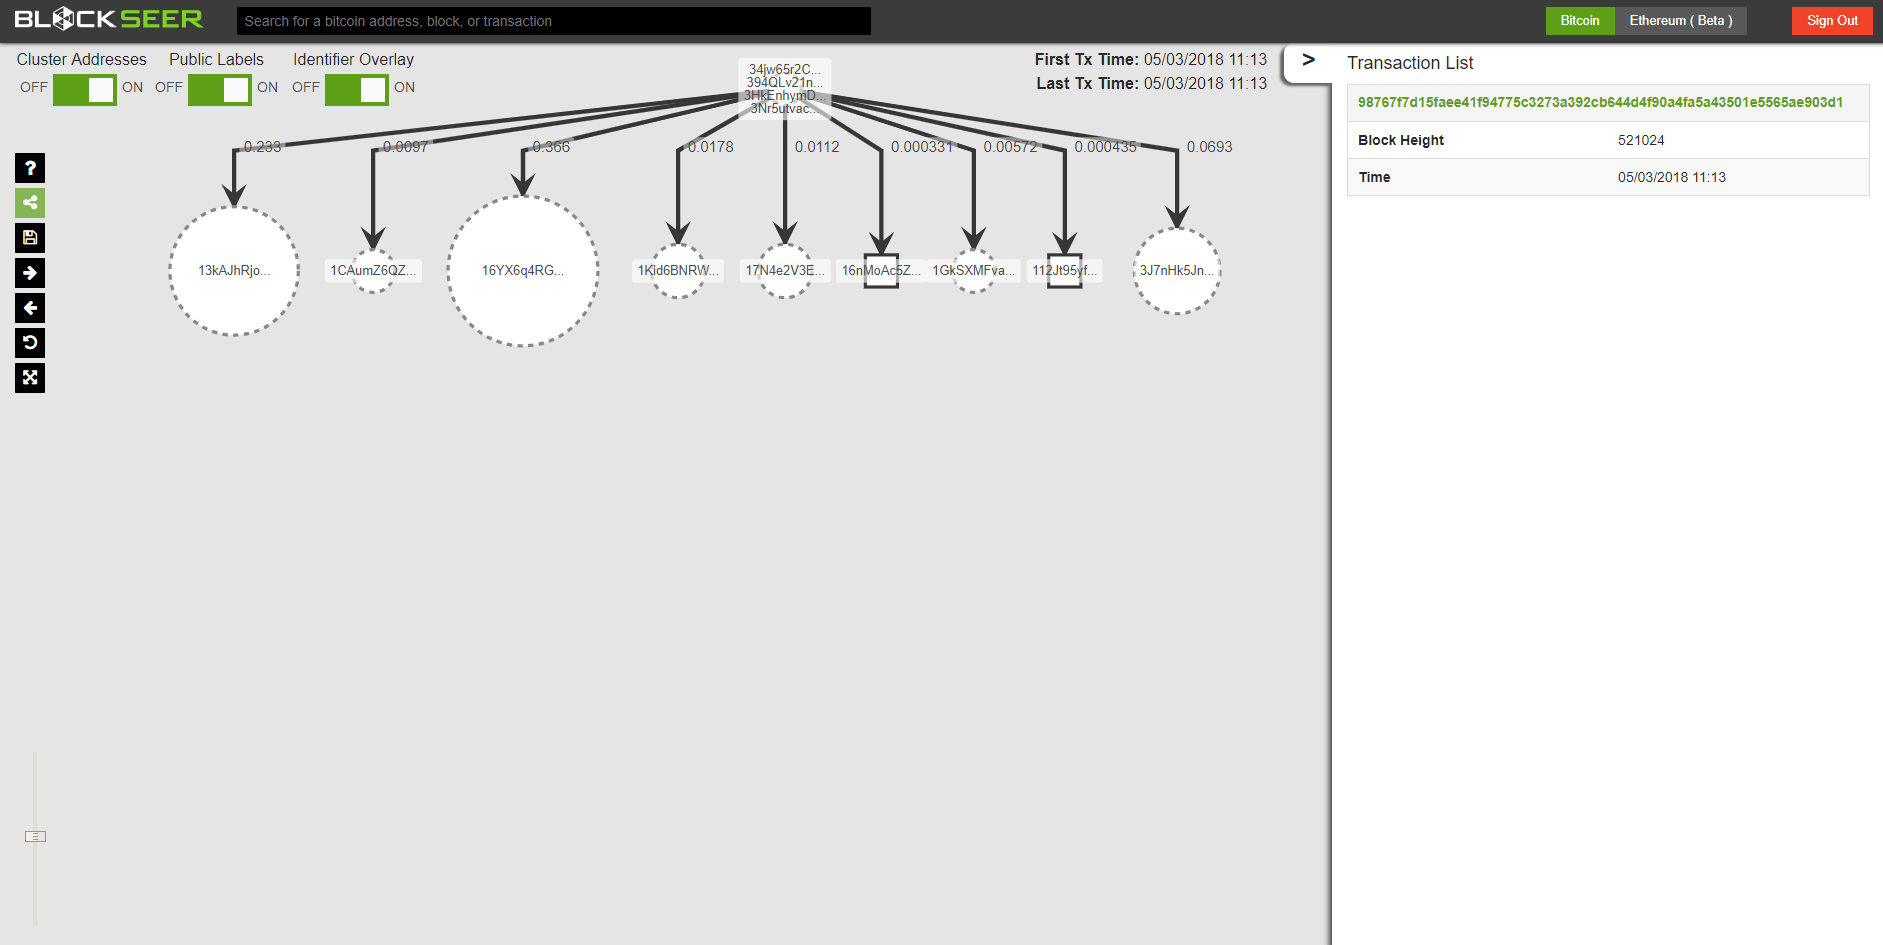
\includegraphics[width=\textwidth]{related_blockseer}
        \caption{Blockseer}
    \end{subfigure}

    \begin{subfigure}[b]{0.45\textwidth}
        \centering
        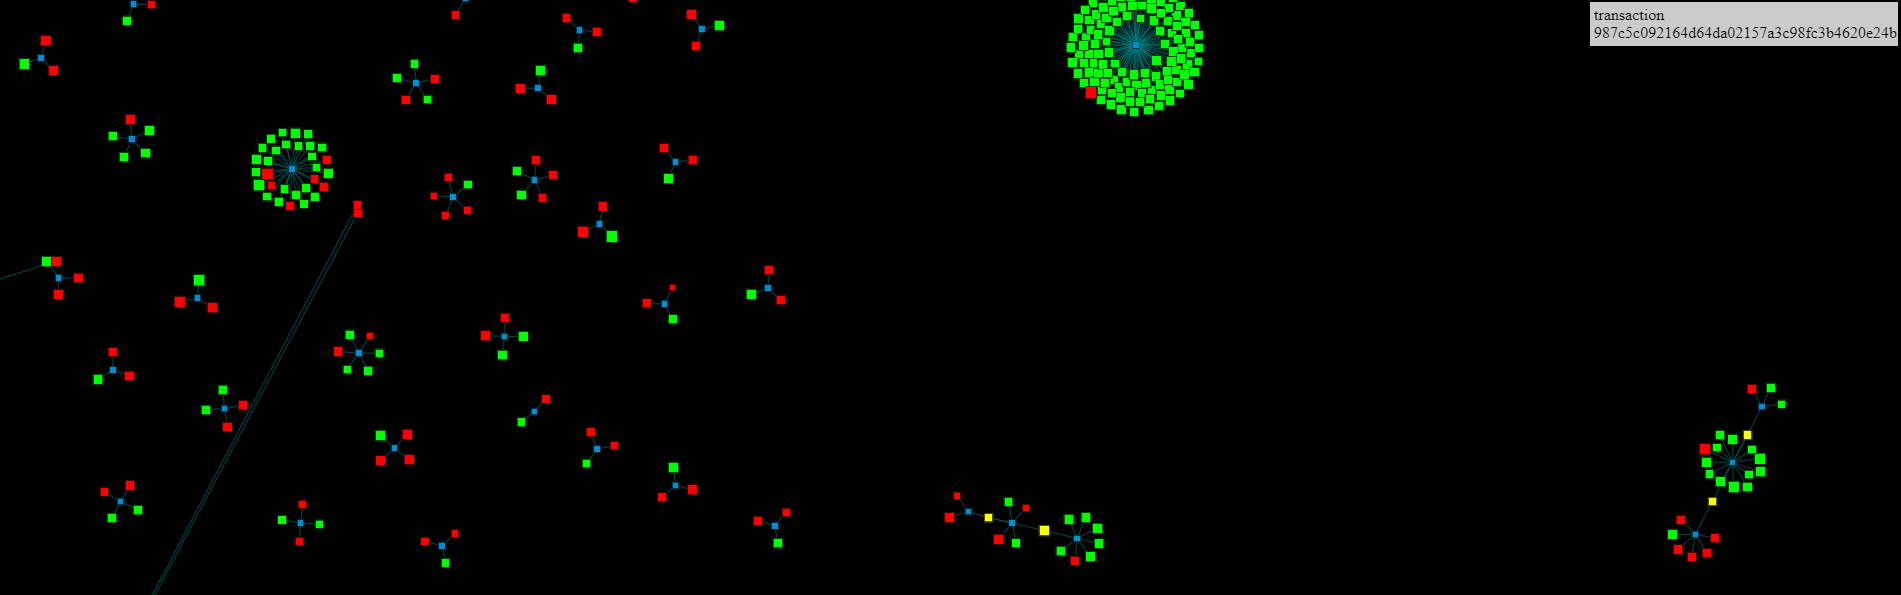
\includegraphics[width=\textwidth]{related_dailyblockchain}
        \caption{DailyBlockchain}
    \end{subfigure}
    \hfill
    \begin{subfigure}[b]{0.45\textwidth}
        \centering
        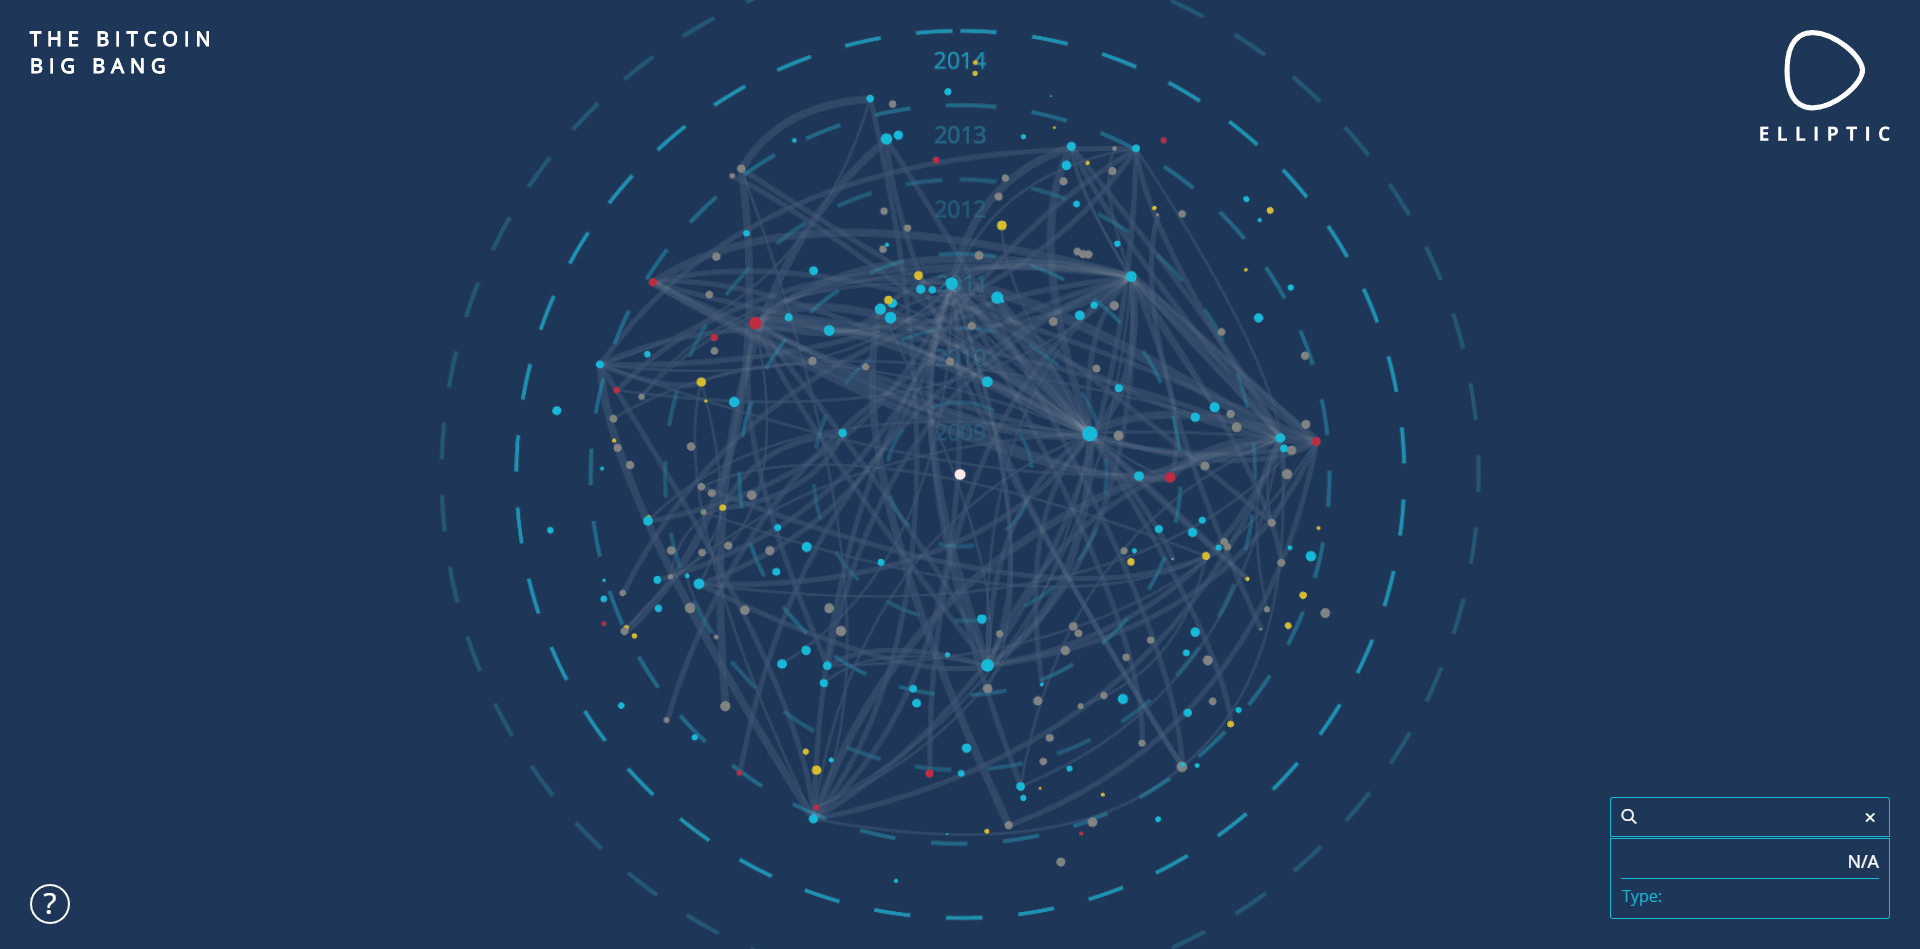
\includegraphics[width=\textwidth]{related_elliptic}
        \caption{Elliptic}
    \end{subfigure}

    \begin{subfigure}[b]{0.45\textwidth}
        \centering
        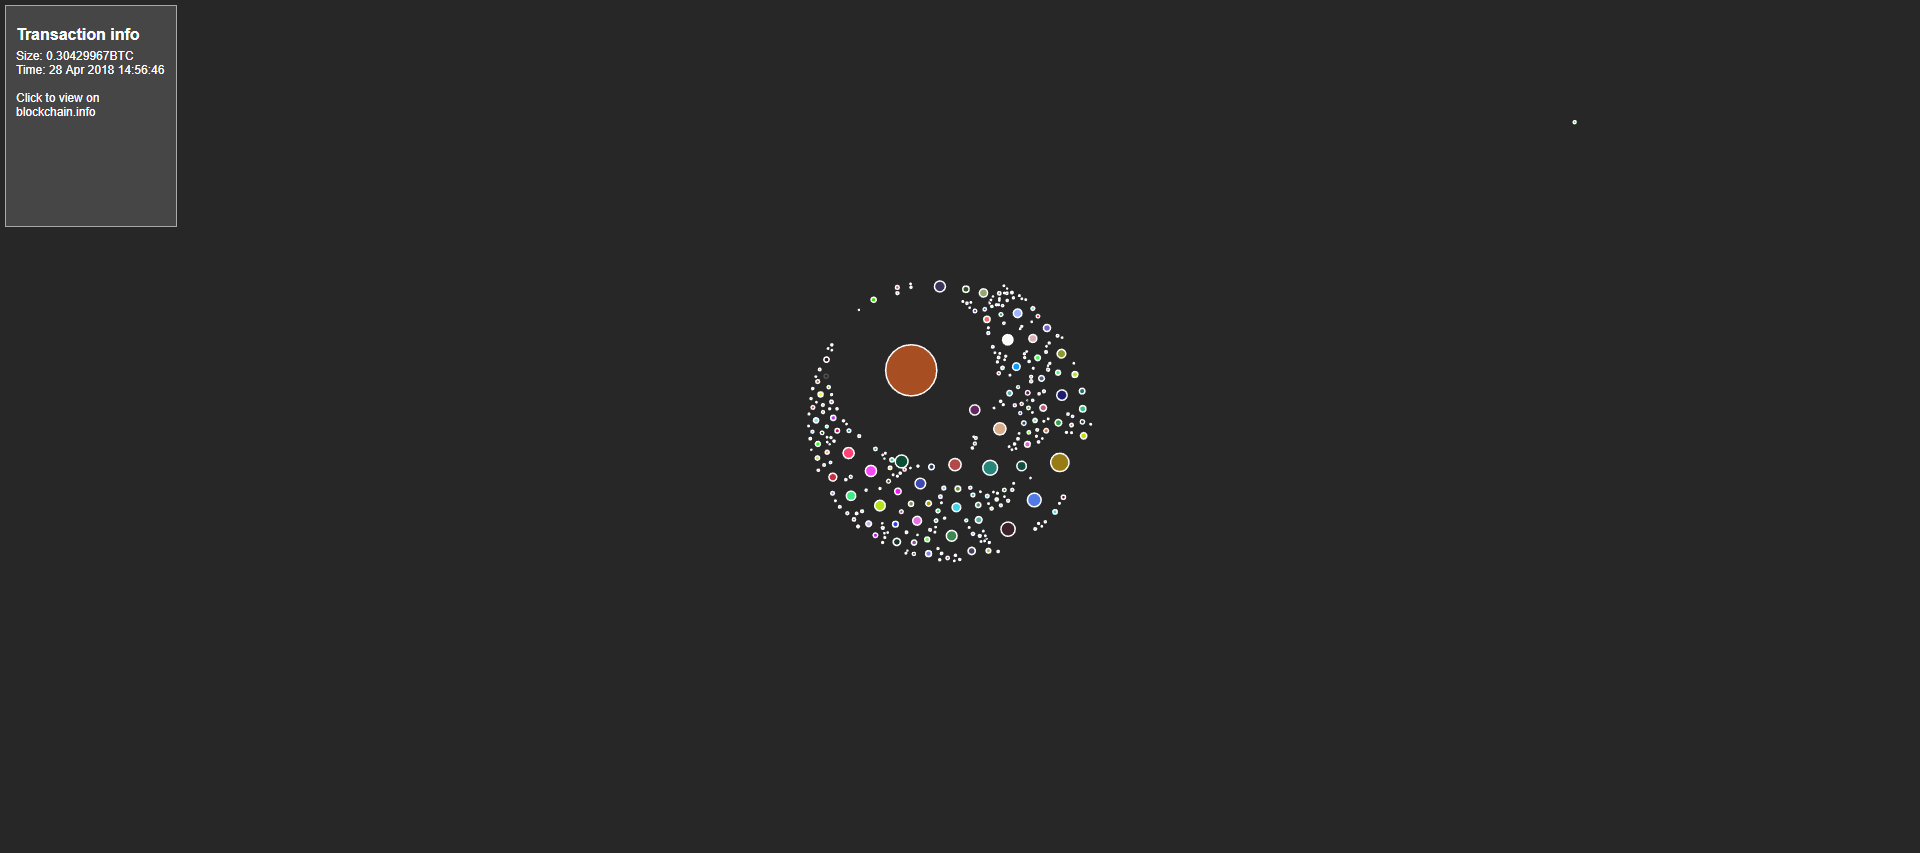
\includegraphics[width=\textwidth]{related_interaqt}
        \caption{Interaqt}
    \end{subfigure}
    \hfill
    \begin{subfigure}[b]{0.45\textwidth}
        \centering
        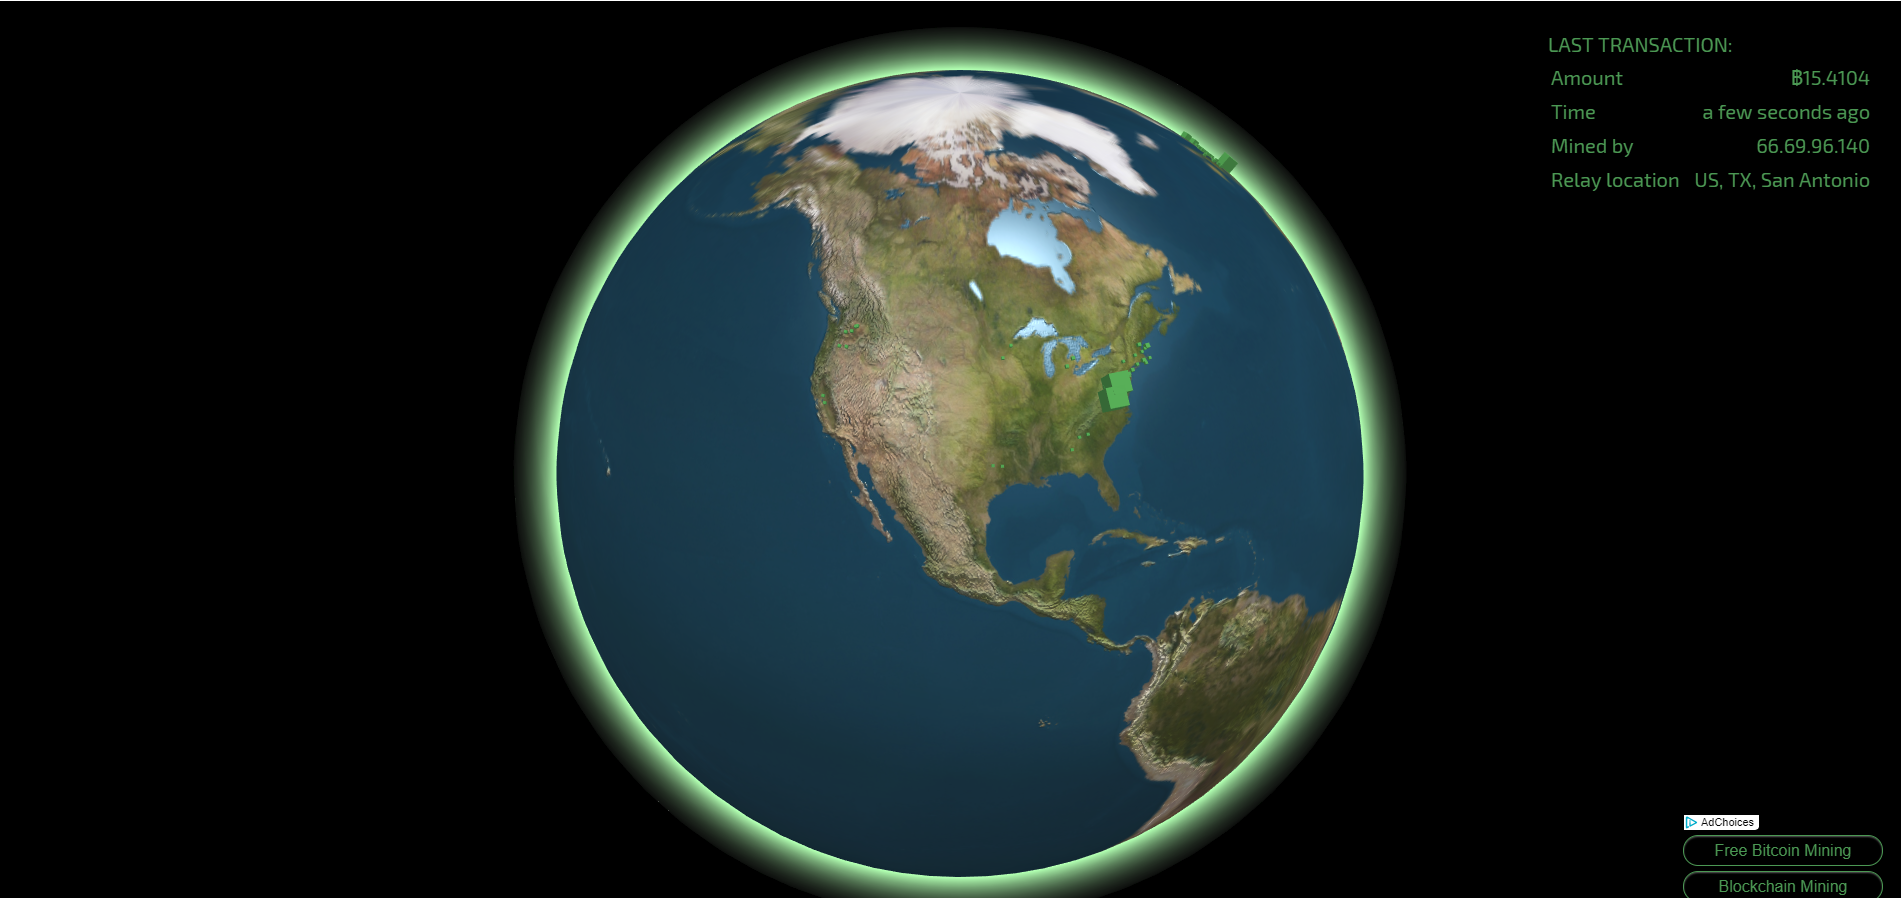
\includegraphics[width=\textwidth]{related_liveglobe}
        \caption{Live Globe}
    \end{subfigure}

    \caption{Visualization of Bitcoin.}
    \label{fig:visualization of bitcoin}
\end{figure}

In addition to the 2D and 3D animations of the visualization of Bitcoin, there are applications which use tabular methods as the presentation of blockchains. Blockchain \cite{blockchain} and Etherscan \cite{etherscan} displayed the information of transactions and blocks in detail on Bitcoin and Ethereum networks. The results of them are demonstrated in Figure \ref{fig:tabular visualization}.

\begin{figure}[htb]
    \centering
    \begin{subfigure}[b]{0.45\textwidth}
        \centering
        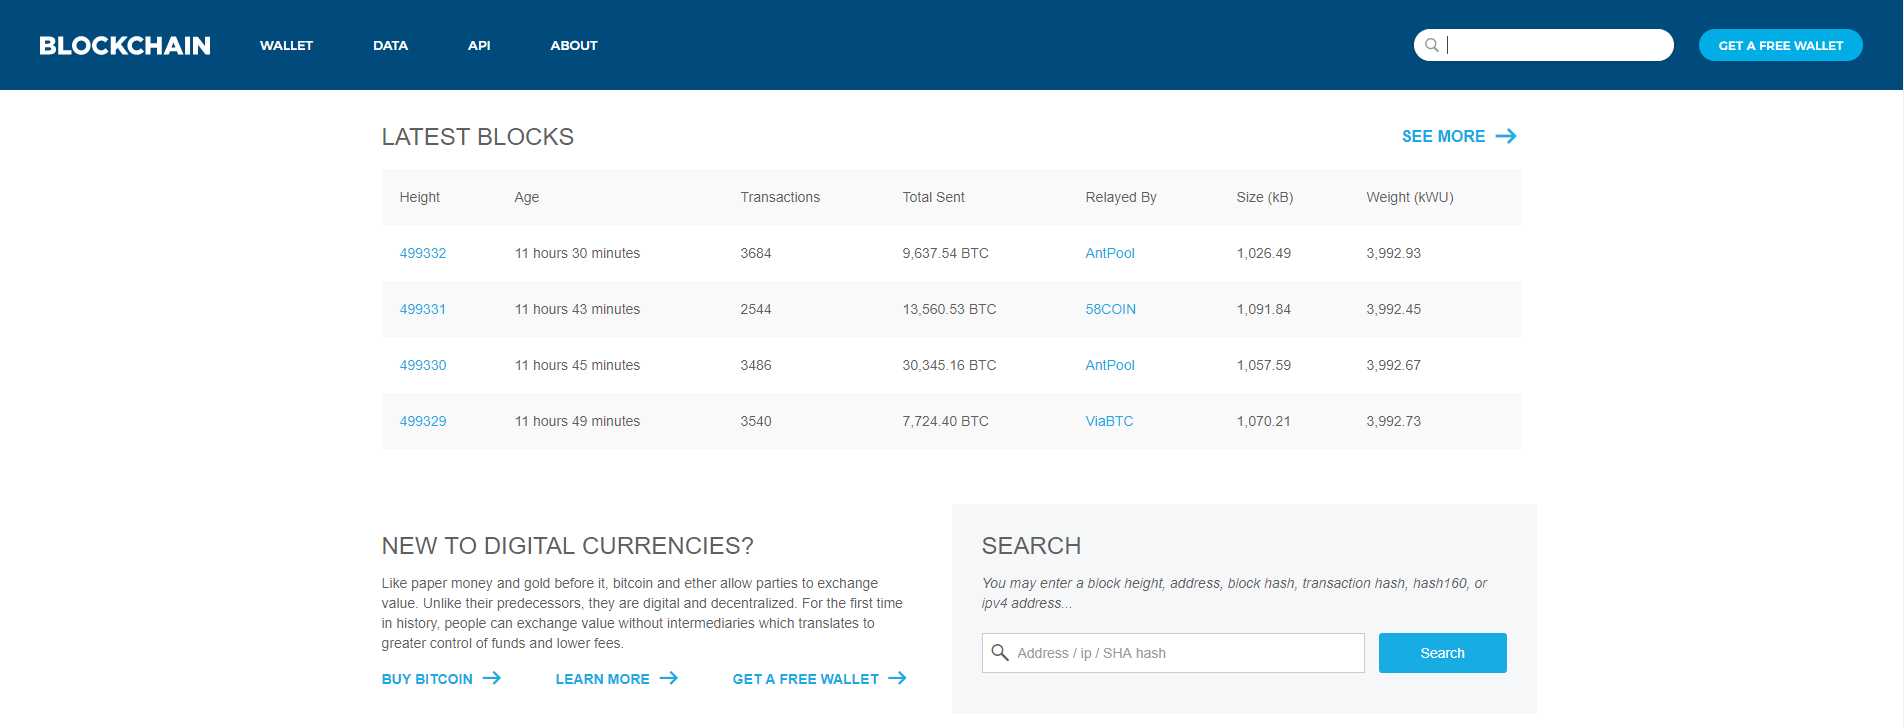
\includegraphics[width=\textwidth]{related_blockchain}
        \caption{Blockchain}
    \end{subfigure}
    \hfill
    \begin{subfigure}[b]{0.45\textwidth}
        \centering
        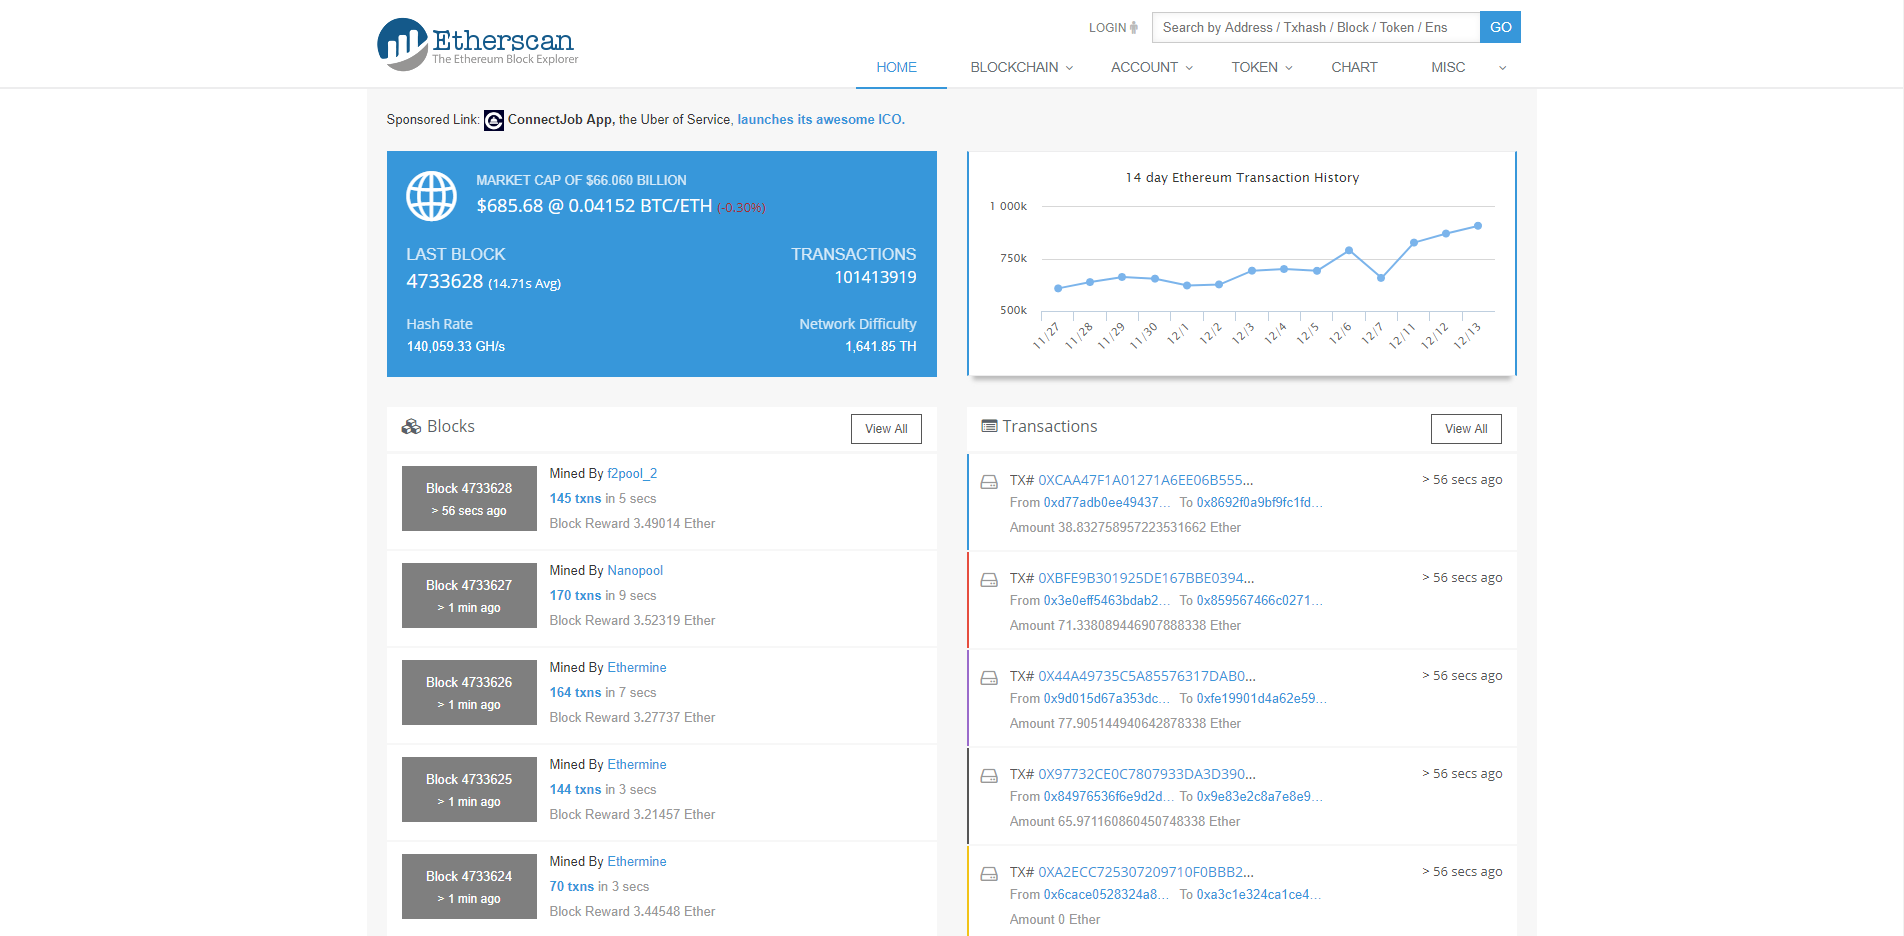
\includegraphics[width=\textwidth]{related_etherscan}
        \caption{Etherscan}
    \end{subfigure}

    \caption{Tabular Visualization.}
    \label{fig:tabular visualization}
\end{figure}

In short conclusion, although the above tools and applications showed amazing visualization methods of blockchains, their goals were to provide the static information and statistics instead of the dynamic mining processes that happened in a blockchain system. It is difficult to gain valuable understandings about the complex and dynamic mining processes in these applications.

\section{Analysis of Transactions}

As Bitcoin is the most popular and famous blockchain network currently, it is worth to explore the patterns of transactions and blocks to prevent malicious abuse of blockchain services. The nodes and transactions are anonymous on blockchain networks, so the recognition of patterns can be challengeable. Here we present some analysis methods and visualization technologies that can identify the relationships between nodes and transactions in time series on Bitcoin networks.

\begin{itemize}
    \item \textbf{BitConeView: Visualization of Flows in the Bitcoin Transaction Graph} \cite{Battista2015} \\
        Giuseppe Di Battista et al. provided a visualization tool called BitConeView that analyzed the flows of bitcoins in the transactions by timestamps. It can be used to analyze the patterns of the flows of bitcoins and locate tainted transactions.
    \item \textbf{Blockchain Explorer: An Analytical Process and Investigation Environment for Bitcoin} \cite{Kuzuno2017} \\
        To prevent the criminal activities and illegal behaviors that abuse the services of Bitcoin, Hiroki Kuzuno et al. proposed an analyzing system which managed the data and statistics of blockchains for the usages of law enforcement investigation and training.
    \item \textbf{Visualizing Dynamic Bitcoin Transaction Patterns} \cite{McGinn2016} \\
        Dan McGinn et al. focused on visualizing transactions of Bitcoin from the top-down viewpoint. The visualization of the large scale of data provided domain experts and the general public a tool to analyze and identify the transaction patterns with big data visualization methods.
    \item \textbf{Bitcoin Visualization} \cite{Saublet2015} \\
        The visual analytics tool that was proposed by Loïs Saublet enabled economists to analyze the metrics and actors in Bitcoin and provided good user experience by working together with end users.
    \item \textbf{Bitcoin Transaction Graph Analysis} \cite{Fleder2015} \\
        Michael Fleder et al. proposed a graph-analysis framework that could analyze the relationships between public addresses and transactions. It can be used to match candidate Bitcoin transactions with the transactions in the reality. As a result, it demonstrated that the transactions are not entirely anonymous on Bitcoin network.
    \item \textbf{Exploring the Bitcoin Network} \cite{Baumann2014} \\
        The method proposed by Annika Baumann et al. employed graph mining algorithms to analyze the relationship of network usage and exchange rate. It served as the basis for the analysis of the anonymity and economic relationships in Bitcoin network.
\end{itemize}

In summary, the goals of the above tools and methods were to analyze the patterns and relationships of transactions and blocks. The results of the visualization of the above literature served as bases and presentations for the analysis. 

\section{Analysis of Consensus Protocols}

To analyze the network conditions of the proof-of-work based blockchain system, Amitai Porat et al. \cite{Porat} provided an application that was based on Ethereum platform. It simulated the asynchronous mining activities and network latency and provided a real-time analysis of the blockchain system. They presented the potential applications of blockchain technology through the analysis.

The main difference to our work is that we assume that miners have individual mining strategies instead of solving the same puzzles asynchronously. Therefore, there are miners who are able to solve the puzzles faster than the others under the same computing power, but they may suffer lower mining rewards. The combination of different mining strategies and delays of networks makes the visualization of the blockchain system dynamic and interesting, and it is suitable for researchers to find the influences of them on the blockchain system. 

Moreover, Amitai Porat et al. focused on the potential applications of Ethereum platform. On the other hand, our work emphasized the continuous mining processes while miniers have different mining strategies and suffer from delays of networks. 

\section{Our Approach}

To focus on the dynamic mining activities, our tool provides a clear, real-time visualization of mining processes that cannot be achieved by the above online nalysis tools. Through our visualization, users can observe the mining processes step by step. Moreover, our visualization is independent of specific blockchain platforms, e.g., Bitcoin and Ethereum, because we built a simple simulation of the blockchain system by ourselves. Therefore, we can concern the mining processes, which is the most important activities in a proof-of-work based blockchain system.

\begin{figure}[htb]
    \centering
    \begin{subfigure}[b]{1\textwidth}
        \centering
        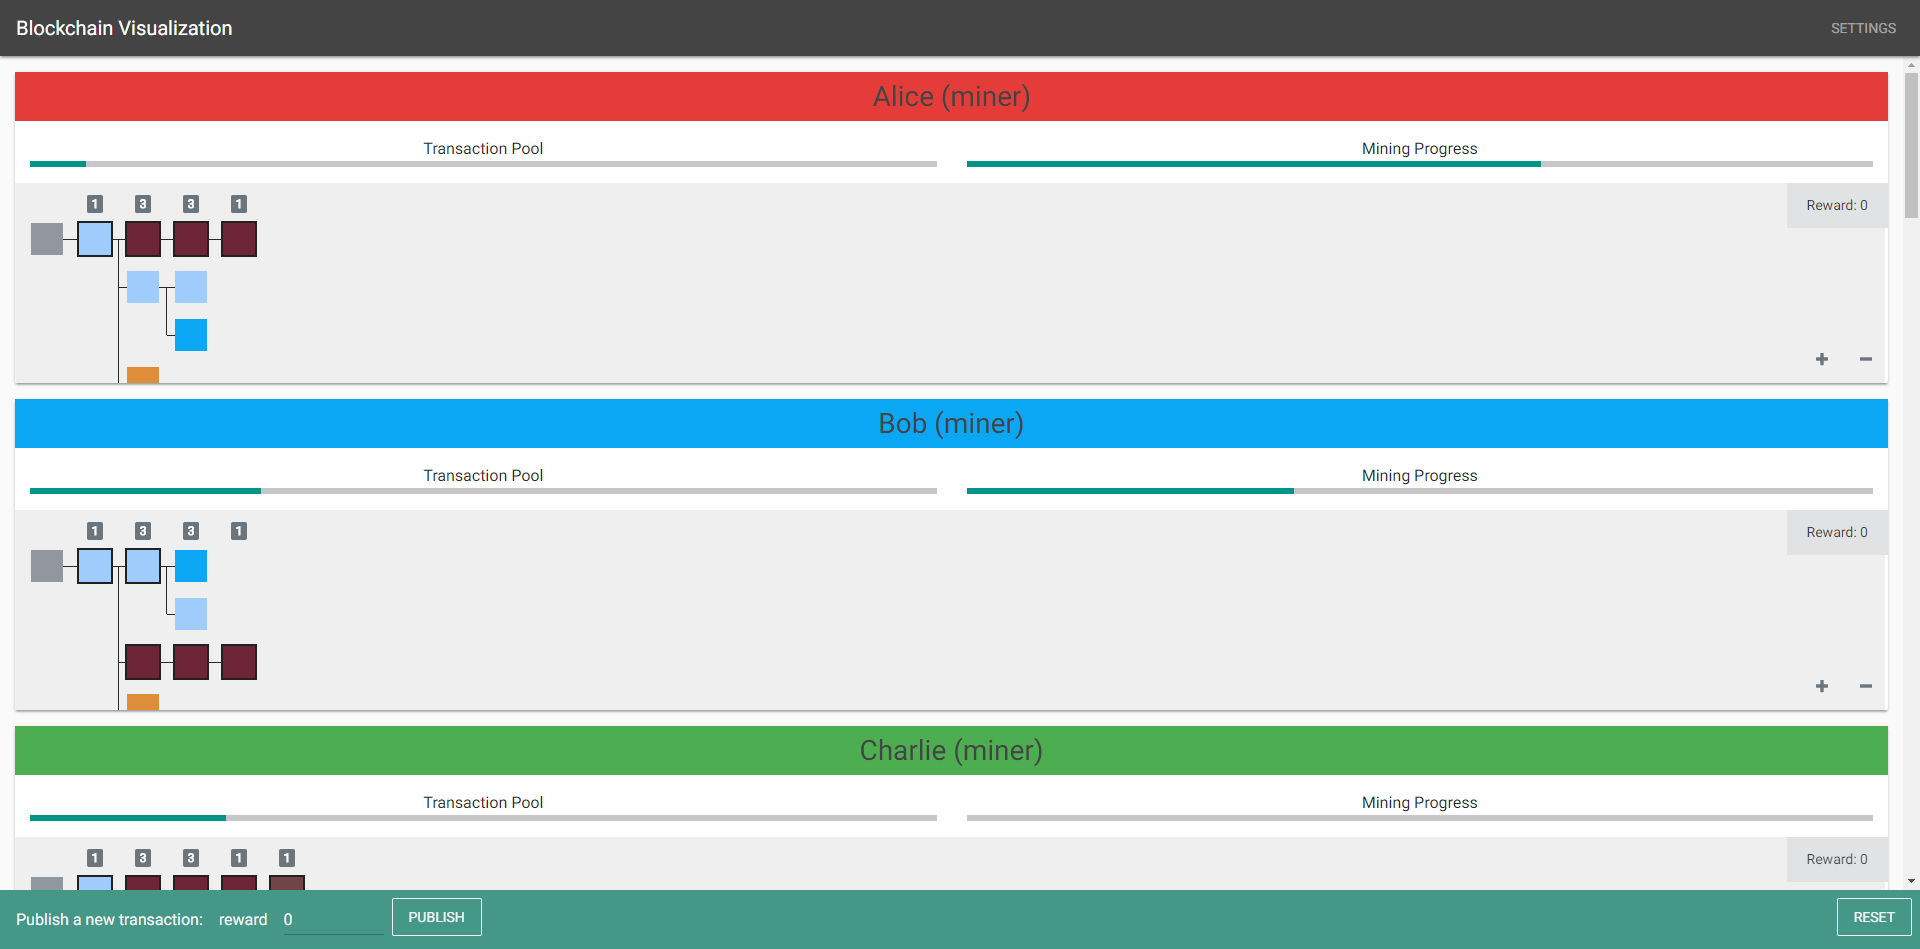
\includegraphics[width=\textwidth]{related_us1}
        \caption{Mining Step 1}
    \end{subfigure}

    \begin{subfigure}[b]{1\textwidth}
        \centering
        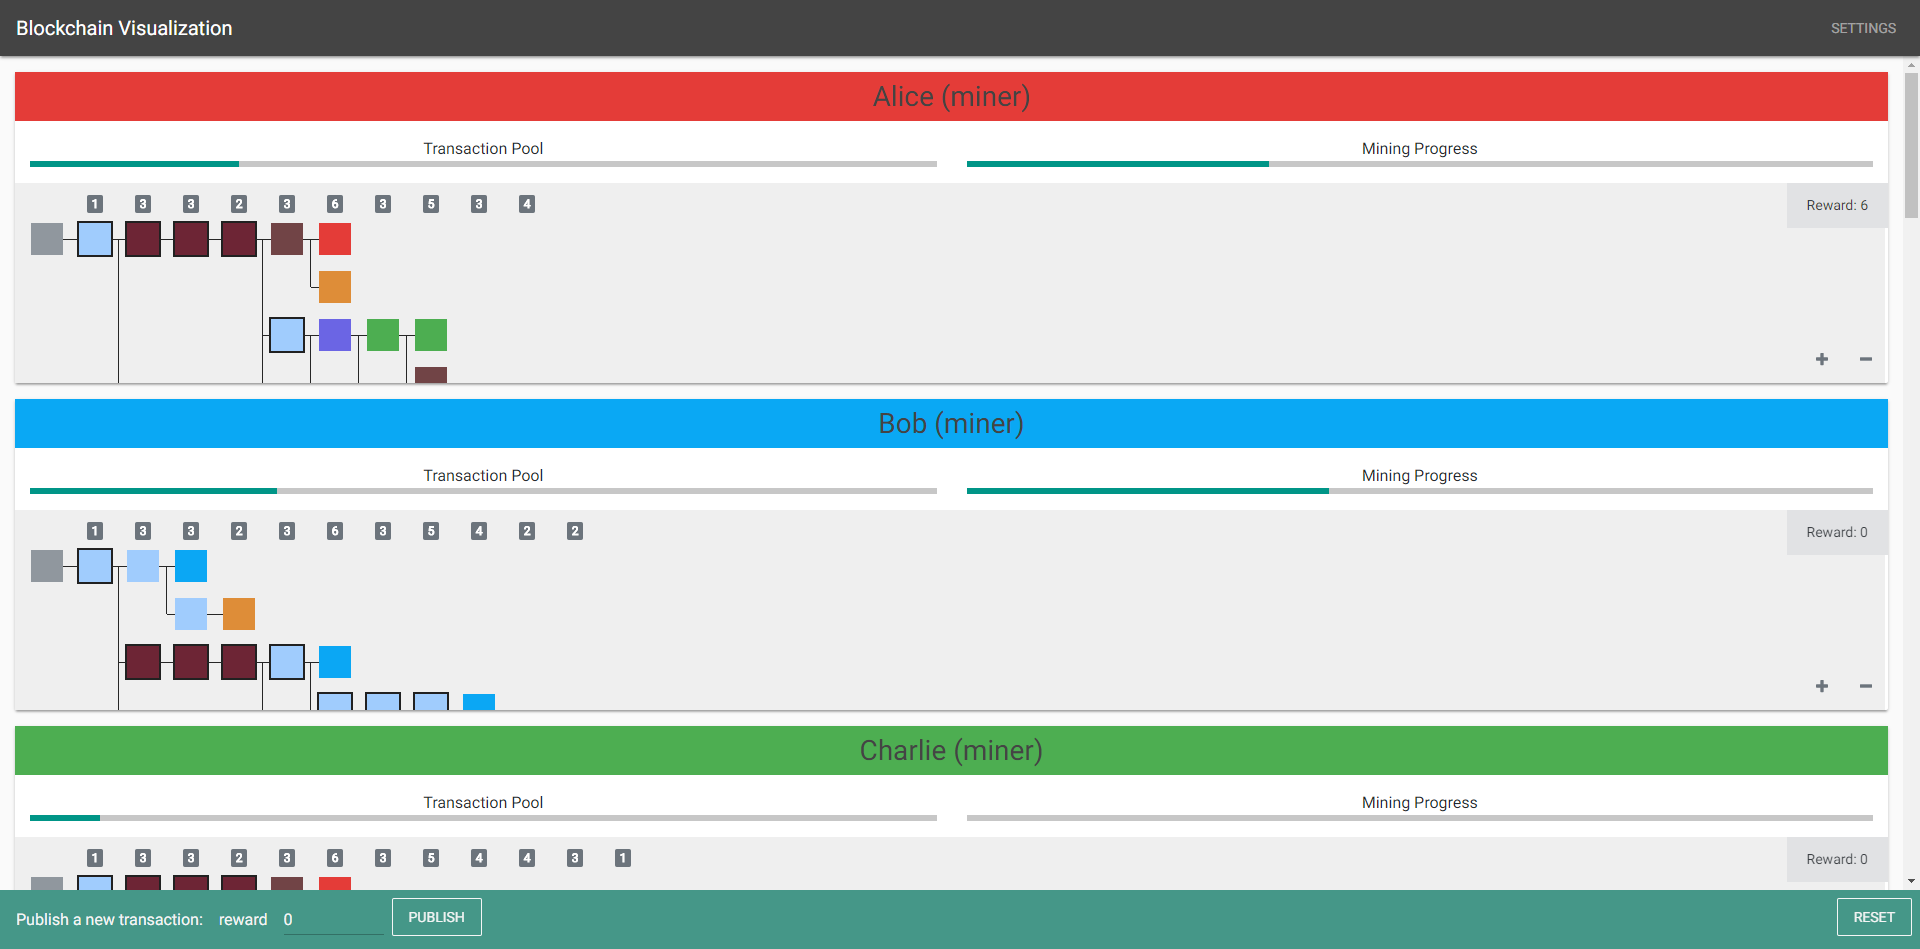
\includegraphics[width=\textwidth]{related_us2}
        \caption{Mining Step 2}
    \end{subfigure}

    \caption{Steps of Mining.}
    \label{fig:steps of mining}
\end{figure}

As we can see in Figure \ref{fig:steps of mining}, the tree structure of the blockchain keeps growing while the mining activities continue. There is a former project called “Kooperative Music Box” \cite{musicbox}, which was developed by Fraunhofer Blockchain-Labor. It used shapes and colors to distinguish different blocks and transactions which were generated by different nodes. The basic visualization ideas of our project are inspired by this application.

Our project aims to visualize all the dynamic mining processes that could happen in a blockchain system, with the factors of the different mining strategies and the delays of networks. This distinguishes our project to all the projects mentioned before. Therefore, our project is worthwhile as a contribution and trial to the blockchain research area.


\chapter{Blockchain System}
Before continuing to the visualization part, it is worth to define the blockchain system that we refer to. Because the research of blockchain technology is still in progress, there are different methods and approaches used to construct a blockchain system. In this chapter, we introduce the ideas of the blockchain system that serves as the basis of the visualization.

\section{Data Types}

There are only two types of data structures that are used in the blockchain system: \textit{transactions} and \textit{blocks}. They are published and received by nodes continuously in the same blockchain network. A transaction contains information that is used in the blockchain system, such as a trade of cryptocurrecy or a shopping item. A block contains a number of transactions that are mined by a miner, and blocks are chained together to form a tree structure that represents the blockchain data structure. The transactions that are included in a block are considered to be confirmed if the block is at the longest blockchain.

\begin{table}[htb]
    \centering
    \begin{tabular}{ M{2cm}|m{8cm} } 
        \hline
        \multicolumn{2}{c}{\textbf{Transaction}} \\
        \hline
        \textit{Properties} & \multicolumn{1}{c}{\textit{Description}} \\
        \hline
        ID & the hash value of the transaction. \\ 
        type & is always “transaction”. \\ 
        timestamp & the time that the transaction is created. \\ 
        reward & the number of rewards that the miner will receive. \\ 
        privilege & to prevent the starvation of the transaction. \\ 
        \hline
    \end{tabular}
    \caption{Properties of Transactions.}
    \label{tab:properties of transactions}
\end{table}

For transactions (Table \ref{tab:properties of transactions}), the properties contain the ID, the type, the timestamp, the reward, and the privilege. The ID represents the hash value of the transaction in a blockchain system. Here we use 8 random characters and digits to simplify the representation. The type indicates that the data is a valid transaction data structure. The timestamp is decided at the time the transaction is created. 

The reward and the privilege are related to the mining strategies. The \textit{value} of a transaction is the sum of the reward and the privilege, as the equation \ref{eq:transaction value} states.

\begin{equation} \label{eq:transaction value}
    value = reward + privilege
\end{equation}

Miners can set the minimum value of transactions that are qualified to be mined. The reward is the number of money that will be assigned to the miner as a motivation because miners solve puzzles in a proof-of-work based blockchain system. The privilege is set to 0 when a transaction is created, and it is added by a sepcific number if the transaction is not selected to be mined each time during the mining activities. That is, the privilege prevents the transaction from starvation, i.e., the transaction will not have chance to be mined because of its low reward.

To explain the value of transactions clearly, suppose that a transaction with reward of 5 was generated and published, and a miner, Alice, received this transaction. At this time, Alice set the privilege of this transaction to 0. Now the total value of this transaction is 

\begin{gather*}
    reward = 5 \\
    privilege = 0 \\
    value = reward + privilege = 5 + 0 = 5
\end{gather*}

Assume that Alice decides to mine a block, but she does not select this transaction as one of the candidates because Alice expects that the minimum value of transactions should be 6. Therefore, the privilege of this transaction is added by a sepcific number (1 in this example). Now the value of this transaction is

\begin{gather*}
    reward = 5 \\
    privilege = 1 \\
    value = reward + privilege = 5 + 1 = 6
\end{gather*}

Thus, when Alice decides to mine a block next time, she will select this transaction as one of the candidates because the value of this transaction is not less than 6. It demonstrates that the privilege prevents this transaction from starvation. Actually, we design this mechanism because a transaction should not be ignored forever in a real blockchain system such as Bitcoin, even if the reward of the transaction is very low.

\begin{table}[htb]
    \centering
    \begin{tabular}{ M{2cm}|m{8cm} } 
        \hline
        \multicolumn{2}{c}{\textbf{Block}} \\
        \hline
        \textit{Properties} & \multicolumn{1}{c}{\textit{Description}} \\
        \hline
        ID & the hash value of the block. \\ 
        type & is always “block”. \\ 
        timestamp & the time that the block is created. \\ 
        miner & the public address of the miner. \\ 
        previous & the hash value of the previous block. \\ 
        layer & indicates the position of the block in the blockchain. \\ 
        color & the color of the block. \\ 
        transactions & an array of transactions. \\ 
        \hline
    \end{tabular}
    \caption{Properties of Blocks.}
    \label{tab:properties of blocks}
\end{table}

For blocks (Table \ref{tab:properties of blocks}), the properties contain the ID, the type, the timestamp, the miner, the previous, the layer, the color, and the transactions. The ID represents the hash value of the block in a blockchain system. Here we use also 8 random characters and digits as the hash value. The type indicates that the data is a valid block data structure. The timestamp is decided at the time the block is created. The miner represents the public address of the miner who mined this block, and it is a 8 random characters and digits. The previous contains the ID of the previous block that is chained in the same blockchain. The transactions includes an array of transactions, and the total reward of the block is the sum of these transactions.

The layer and color are useful for the visualization of the blockchains. The layer defines the position of a block in a blockchain and ensures that the visualization of the structures of blockchains between different nodes is the same. The color distinguishes the miner of the blocks in the visualization. The blocks with the same color mean that these blocks are from the same miner and vice versa.

\begin{figure}[htb]
    \centering
    \begin{subfigure}[b]{0.4\textwidth}
        \centering
        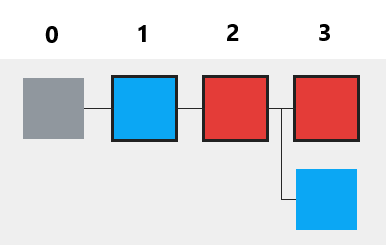
\includegraphics[width=\textwidth]{blockchain_block1}
        \caption{Alice's blockchain}
    \end{subfigure}
    \hfill
    \begin{subfigure}[b]{0.4\textwidth}
        \centering
        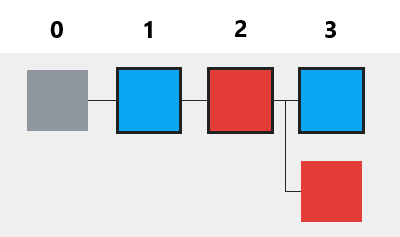
\includegraphics[width=\textwidth]{blockchain_block2}
        \caption{Bob's blockchain}
    \end{subfigure}

    \caption{Visualization of Blocks.}
    \label{fig:visualization of blocks}
\end{figure}

To illustrate the positions of blocks in the visualization, suppose that there are two miners, Alice and Bob. Alice's color is red, and Bob's color is blue. According to figure \ref{fig:visualization of blocks}, Alice and Bob mined two block individually. The grey block represents the genesis block. The red blocks are from Alice, and the blue ones are from Bob. The number of layers of the blocks are indicated on the top of the figures. In each layer, the number of different color of blocks are the same. However, the vertical positions of the blocks are not always the same. It is because that each miner received the same block at different time. In this example, Alice and Bob put their own blocks on the top of the layer because they received their own blocks earlier. As a result, the layer guarantees that the blockchain data structures are the same between every node.

\section{Nodes}

In the blockchain system, there are three types of nodes that communicate with each other. 
\begin{itemize}
    \item \textbf{Transaction Generator}
        The transaction generator is unique in the blockchain system. It is responsible for generating and publishing transactions to miners.
    \item \textbf{Miner}
        Miners are the most important nodes in the visualization because they mine and publish blocks according to their individual mining strategies. Each miner has their own transaction pools which contain all the pending transactions. Because the transaction generator publishes the transactions through the unstable network, each miner has different sets of pending transactions at the same time.
    \item \textbf{Nonminer}
        Nonminers only receive blocks from miners and publishes blocks to their neighbors.
\end{itemize}

The blockchain data structures of different nodes are not always the same since the blockchain system is active. It is because of the delays of the unstable network between different nodes, and the visualization of the different blockchain data structures is the main feature of our application. For example, figure \ref{fig:visualization of blocks} shows the difference between Alice's and Bob's blockchain data structures.

\begin{figure}[htb]
    \centering
    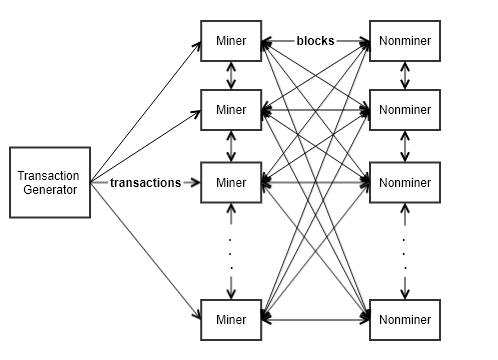
\includegraphics[width=\textwidth]{blockchain_nodes}
    \caption{Relationships of Nodes.}
    \label{fig:relationship of nodes}
\end{figure}

The relationship of different types of nodes is shown in figure \ref{fig:relationship of nodes}. In the beginning, the transaction generator publishes transactions to the miners. When a miner mines a block, he/she will publish the block through his/her neighbors. Other miners and nonminers will again publish the received block to their neighbors after they received the block from other miners or nonminers. If a miner or a nonminer receives duplicate blocks, then he/she will discards the block to prevent sending and receiving the same block repeatedly.

\section{Unstable Networks}

The networks between each node are unstable due to the peer-to-peer networks. Therefore, the publishes of transactions and blocks suffer delays. Because of the unstable network, forks happen in the visualization of the blockchains while several miners are mining simultaneously. Moreover, nodes could be partitioned into different groups and compete with other groups.

\section{Mining Strategies}

Every miner has different mining strategies. There are four parameters that are related to the mining strategies. The first is the amount of time that a miner should spend on mining. It represents the computing power of a miner. The second is the minimum value of transactions that are considered to be mined into a block. It is the threshold of the values of transactions which are qualified to be selected when the miner decides to mine a block. The third is the number of transactions in a block. That is, it is the size of a block. The sizes of blocks are always the same for the same miner. The fourth is the minimum number of pending transactions in the transaction pools. It prevents that a miner responds too slowly in the blockchain system when the minimum value of transactions is set by a large number.

The four parameters make the mining behaviors of the miners different from each other. The influences of mining strategies to the blockchain system under specific environment can be identified clearly through the visualization.

\section{Consensus Protocols}


\chapter{Implementation}
In this chapter, 

\section{Architecture}

\begin{figure}[htb]
    \centering
    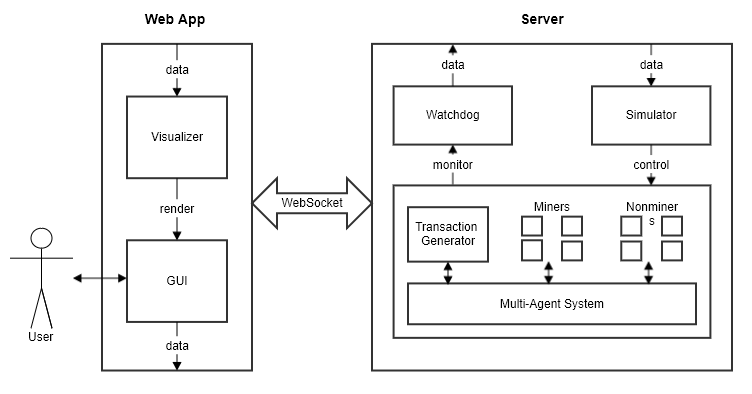
\includegraphics[width=\textwidth]{impl_architecture}
    \caption{Architecture.}
    \label{fig:architecture}
\end{figure}

Figure \ref{fig:architecture} shows the whole architecture of the visualization application. The architecture contains a web app and a server, which are connected with WebSocket. WebSocket technology makes the real-time communications between the web app and the server possible, as the visualization of the real-time mining processes is necessary. The user can interact with the web application through the graphical user interface.

The server maintains the blockchain system. It is composed of three components.

\begin{itemize}
    \item \textbf{Blockchain System} \\
        The blockchain system is based on a multi-agent system. It cointains a transaction generator, multiple miners, and multiple nonminers. The multi-agent system provides communications for these nodes.
    \item \textbf{Simulator} \\
        The simulator is responsible for receiving data from the client side and controlling the blockchain system.
    \item \textbf{Watchdog} \\
        When the blockchain data structures change in the blockchain system, the watchdog will catch these changes, and send them to the web app. 
\end{itemize}

Since the nodes on the blockchain network can be regarded as agents on a multi-agent system, we decided to contruct the blockchain system with a multi-agent system framework. Here, We choose a web-based multi-agent system framework called Eve \cite{eve}. The main features of Eve are stated below.

\begin{itemize}
    \item \textbf{Robustness} \\
        The agents are decoupled and can be maintained independently. Thus, the whole system is still active even an agent fails.
    \item \textbf{Flexibility} \\
        It is flexible to add or remove agents.
    \item \textbf{Reduced complexity} \\
        The complexity of the distributed software design is lower.
    \item \textbf{Scalability} \\
        The limitation of the number of agents does not exist, so the scalability can grow rapidly.
\end{itemize}

In addtion, Eve provides reliable communications with JSON-RPC protocols \cite{jsonrpc}. Therefore, agents can send and understand the JSON format data between each other, and they can be maintained independently in anywhere, e.g., on the cloud or desktops. Eve is an open source project which is implemented in JavaScript, and it is easy to learn. As a result, Eve allows us to construct a distributed blockchain system without worrying about the technical problems such as asynchronous and locking problems.

The server is built in Node.js with Express framework because of it is based on the same programming language of Eve. During the runtime, a transaction generator, miners, and nonminers can be instantiated and destroyed at any time thanks to the flexibility of Eve.

The web application is responsible for the visualization and the interactions with users. There are two components in the web application.

\begin{itemize}
    \item \textbf{Visualizer} \\
        The visualizer is responsible for rendering the visualization of blockchains when it is notified by the watchdog. It receives the data of transactions and blocks from the server and renders them appropriately on the HTML documents.
    \item \textbf{Graphical User Interface} \\
        The GUI provides an index page and a settings page. The index page is for the visualization part, and the settings page displays all the defined parameters in the blockchain system. More details can be refered to \ref{}.
\end{itemize}

The visualization is based on Three.js, a JavaScript framework for rendering 2D and 3D graphics. Three.js uses WebGL as the renderer, and the updating performance is 60 frame per second. The reason to choose Three.js as the visualization framework is that it is an famous open source project, and the community is active. Moreover, Three.js provides basic shapes, e.g., squares and lines, and handles the updating of frames. Therefore, we can focus on optimize the user experience of the visualization without considering the implementation of WebGL.

\section{Simulator}

The simulator is responsible for controlling the blockchain system and handling all the requests from the client. It is unique in the whole system, so it observes to the singleton pattern. The role of the simulator is like a "door" as it is the only gate to communicate with the blockchain system.

After the blockchain system starts, the simulator initializes the status of the blockchain system, i.e., it instantiates necessary nodes according to the configuration. The waiting list of transactions in the transaction generator and the blockchain data structures of miners and nonminers are initialized by the simulator. 

When the user wants to change the parameters, i.e., mining strategies and delays of networks, or the visualizer needs the information of transaction pools and blockchains, the simulator will interact with the blockchain system by setting the parameters or retrieving the required data. The data are sent through WebSocket in real-time.

The simulator is an important component because it hides the details of the implementation of the blockchain system and provides a unique and robust interface for the requests from the client. As a result, it decouples the relationship between the web application and the blockchain system. The detail of the simulator can be refered to \ref{}.

\section{Watchdog}

The watchdog is responsible for monitoring the behaviors of nodes and notifying the visualizer when the data should be updated. It is unique in the whole system, so it also observes to the singleton pattern.

The watchdog watches three kinds of data in the blockchain system.

\begin{itemize}
    \item blockchain data structures
    \item status of transaction pools
    \item status of mining
\end{itemize}

While a miner receives a transaction or a block, a nonminer receives a block, or a miner is solving the puzzle, the watchdog will notify the visualizer in real-time through WebSocket. Therefore, it is guaranteed that the visualization of the data is synchronized with the blockchain system all the time.

With the help of the watchdog, the activities that happened in the blockchain system is recorded completely. Hence, it ensures the correctness of the visualization application. The detail of the watchdog can be refered to \ref{}.

\section{Visualizer}

The visualizer is responsible for rendering the data that are sent from the watchdog. It is the main part of the visualization application because it shows the elegance of visualization. 

Three items are updated by the visualizer continuously.

\begin{itemize}
    \item status bars for transaction pools
    \item status bars for mining
    \item blockchain data structures
\end{itemize}

The status bars for transaction pools and the status bars for mining are auxiliary tools to help the user understand the events that are acctually happening in mining activities. The status bar for transaction pools becomes longer if the pending transactions are growing and vice versa. The status barsfor mining is usually empty, except that the miner is solving the puzzle. It increases each second when the mining activity continuouses. Unlike the real blockchain networks, the time of solving the puzzles is predictable in our visualization application, and it is defined in the parameter of mining strategies. The main area of the visualization is reserved for the blockchain data structures. Squares represent blocks, and they are chained by lines. Different colors of the squares represent the different sources of the blocks. The growth of the blockchain data structures is dynamic and real-time as the mining activities are in progress.

The visualizer expresses fantastic blockchain visualization that is able to attract the user. In addition, it explains the steps of mining processes understandably, even for the viewers who are new to blockchain technology. The detail of the visualizer can be refered to \ref{}.

\section{UML Diagram}

In Figure \ref{fig:class diagram}, it demonstrates the class diagram of the visualization application. The blockchain system is based on the multi-agent system framework Eve. Abstract class \texttt{AbstractNode} inherits from \texttt{Agent} in Eve, and class \texttt{TransactionGenerator}, class \texttt{Miner}, and class \texttt{Nonminer} inherit from it. The blockchain system is controlled by class \texttt{Simulator}, and class \texttt{Watchdog} monitors it and notify class \texttt{Visualizer} when it is necessary to update. Class \texttt{GUI} provides the user interface and is able to interact with \texttt{Simulator}. Finally, a helper class \texttt{Hash} provides simulation functionalities of the hash computation. The following contains all the classes that compose the visualization application.

\begin{itemize}
    \item \textbf{Agent} (Table \ref{tab:class agent}) \\
        \texttt{Agent} is from the multi-agent system framework, Eve. It establishes the communication channel for the agents. In the implementation, the channel is opened with HTTP protocols. It makes sending and receiving transactions and blocks very simple. 
    \item \textbf{AbstractNode} (Table \ref{tab:class abstractNode}) \\
        It defines the common properties and methods of its children. \texttt{AbstractNode} is an abstract class, so it is not allowed to instantiate instances from it. In contrast, we can create nodes from the children of \texttt{AbstractNode}, i.e., \texttt{TransactionGenerator}, \texttt{Miner}, and \texttt{Nonminer}
    \item \textbf{TransactionGenerator} (Table \ref{tab:class transactiongenerator}) \\
        It is responsible for generating and publishing transactions. There should be only one transaction generator in the blockchain system. Furthermore, the neighbors of the transaction generator only contain the miners.
    \item \textbf{Miner} (Table \ref{tab:class miner}) \\
        \texttt{Miner} is the main role in the blockchain system. It generates and publishes blocks through the blockchain network. Therefore, it controls all the mining processes in the blockchain system.
    \item \textbf{Nonminer} (Table \ref{tab:class nonminer}) \\
        \texttt{Nonminer} represents common users who do not solve complex mathematical puzzles in the blockchain system. The only behavior of nonminers is to receive and publish blocks. Consequently, the miners and the nonminers connect with each other. 
    \item \textbf{Simulator} (Table \ref{tab:class simulator}) \\
        \texttt{Simulator} is the only master of the blockchain system. It is able to add and update nodes, and retrieve information from the blockchain system.
    \item \textbf{Watchdog} (Table \ref{tab:class watchdog}) \\
        \texttt{Watchdog} monitors the blockchain system. When a mining activity starts, it keeps notifying the visualizer until the end.
    \item \textbf{Visualizer} (Table \ref{tab:class visualizer}) \\
        \texttt{Visualizer} uses 3D graphical library to render the blockchain visualization. It maintains all miners' and nonminers' canvases and the mouse events which enable users to drag, zoom in, and zoom out the canvases.
    \item \textbf{GUI} (Table \ref{tab:class gui}) \\
        The graphical user interface is responsible for the interactions with users, including uploading files, updating the blockchain sytem, publishing transactions, and resetting the blockchain system.
    \item \textbf{Hash} (Table \ref{tab:class hash}) \\
        This class generates a sequence of random numbers to simulate the hash functions. It avoids to put lots of computing resources to calculate hash values.
\end{itemize}

\section{Algorithms}
\label{algorithms}

The visualization focuses on the mining processes, i.e., generating and publishing blocks. Hence, the algorithm about mining processes is the key parts of the entire system. The algorithm can be divided into three parts.

\begin{itemize}
    \item Select Candidate Transactions
    \item Mining
    \item Add Block to Blockchain
\end{itemize}

Before a miner starts to mine a block, he/she needs to select a set of candidate transactions for the transaction pool. Thus, these candidate transactions serve as the content of the mined block. After receiving a block, the node will check the layer of the new block, and switch to the new block if the blockchain becomes the longest.

sorted pending transaction

The process of selecting a set of candidate transactions starts with

After determining the candidate transactions, the miner

Receiving a new block triggers the consensus protocol to resolve the longest blockchain.





The mining algorithm determines the most important part of the blockchain system. Miners generate blocks by following the logic of the mining algorithm, but with different parameters that are defined in their own mining strategies. To start mining a block, miners must select a set of pending transactions from their own transaction pools. There are two cases when selecting transactions. If the transaction pool contains too much number of transactions, then the miner ignores the parameter of the minimum value of transactions and selects a set of transactions with the highest values. On the other hand, the miner selects a set of transactions which values are higher than the minimum value of transactions. After the selection of transactions, if the number of selected transactions satisfies the number of transactions that should be included in a block, then the miner will start mining.



Another important algorithm is about the consensus protocol. The algorithm of the consensus protocol is very simple because we do not consider malicious nodes in the blockchain system currently. Therefore, it is only responsible for resolving the longest blockchain. When a node receives a block from other nodes, this algorithm is triggered. If the received block is at a higher layer, i.e., the blockchain becomes longer, then the node will switch the current block to the received block to ensures that it is working on the correct blockchain. Moreover, the transactions of the received block are deleted from the transaction pools because these transactions are not pending anymore.

\clearpage

\begin{figure}[!h]
    \centering
    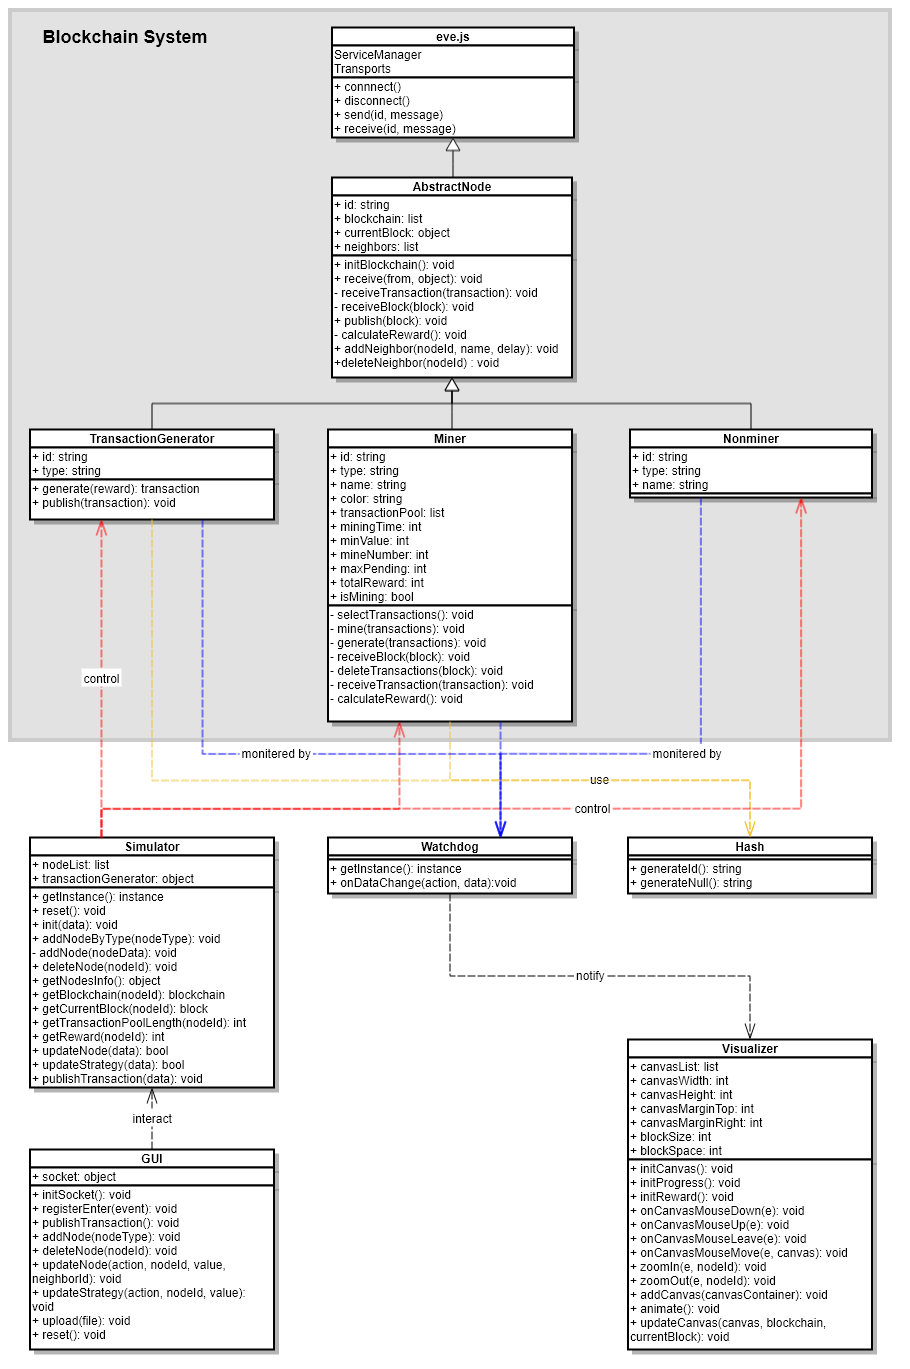
\includegraphics[width=\textwidth]{impl_uml}
    \caption{Class Diagram.}
    \label{fig:class diagram}
\end{figure}

\begin{table}[!h]
    \centering
    \begin{tabular}{ M{3.5cm}|m{8cm} } 
        \hline
        \multicolumn{2}{c}{\textbf{Agent (eve.js)}} \\
        \hline
        \textit{Properties} & \multicolumn{1}{c}{\textit{Description}} \\
        \hline
        transport & communication channels. \\ 
        \hline
        \textit{Methods} & \multicolumn{1}{c}{\textit{Description}} \\
        \hline
        connect & connect with a transport. \\ 
        disconnect & disconnect from a transport. \\ 
        send & send messages to a transport. \\ 
        receive & receive messages from a transport. \\ 
        \hline
    \end{tabular}
    \caption{Class \texttt{Agent}}
    \label{tab:class agent}
\end{table}

\begin{table}[!h]
    \centering
    \begin{tabular}{ M{3.5cm}|m{8cm} } 
        \hline
        \multicolumn{2}{c}{\textbf{AbstractNode}} \\
        \hline
        \textit{Properties} & \multicolumn{1}{c}{\textit{Description}} \\
        \hline
        id & unique in the multi-agent system. \\ 
        blockchain & blockchain data structures. \\ 
        currentBlock & the id of the block which is on the top of the longest blockchain. \\ 
        neighbors & reachable nodes. \\ 
        \hline
        \textit{Methods} & \multicolumn{1}{c}{\textit{Description}} \\
        \hline
        initBlockchain & initialize blockchain data structures. \\ 
        receive & inherit from \texttt{eve.js}. \\ 
        receiveTransaction & define actions of receiving transactions. \\ 
        receiveBlock & define actions of receiving blocks. \\ 
        publish & publish transactions or blocks. \\ 
        calculateReward & calculate the total mining rewards. \\ 
        addNeighbor & add a new node as a neighbor. \\ 
        deleteNeighbor & delete a node from neighbors. \\ 
        \hline
    \end{tabular}
    \caption{Class \texttt{AbstractNode}}
    \label{tab:class abstractNode}
\end{table}

\begin{table}[!h]
    \centering
    \begin{tabular}{ M{3.5cm}|m{8cm} } 
        \hline
        \multicolumn{2}{c}{\textbf{TransactionGenerator}} \\
        \hline
        \textit{Properties} & \multicolumn{1}{c}{\textit{Description}} \\
        \hline
        id & unique in the multi-agent system. \\ 
        type & is always ``generator''. \\ 
        \hline
        \textit{Methods} & \multicolumn{1}{c}{\textit{Description}} \\
        \hline
        generate & generate a transaction. \\ 
        publish & publish a transaction. \\ 
        \hline
    \end{tabular}
    \caption{Class \texttt{TransactionGenerator}}
    \label{tab:class transactiongenerator}
\end{table}

\begin{table}[!h]
    \centering
    \begin{tabular}{ M{3.5cm}|m{8cm} } 
        \hline
        \multicolumn{2}{c}{\textbf{Miner}} \\
        \hline
        \textit{Properties} & \multicolumn{1}{c}{\textit{Description}} \\
        \hline
        id & unique in the multi-agent system. \\ 
        type & is always ``miner''. \\ 
        name & a simple nickname. \\ 
        color & the color of the generated blocks. \\ 
        transactionPool & contain pending transactions. \\ 
        miningTime & computing power. \\ 
        minValue & minimum value of transactions. \\ 
        mineNumber & size of blocks. \\ 
        maxPending & maximum pending transactions. \\ 
        totalReward & total number of rewards. \\ 
        isMining & whether the miner is mining. \\ 
        \hline
        \textit{Methods} & \multicolumn{1}{c}{\textit{Description}} \\
        \hline
        selectTransactions & select pending transactions as candidates. \\ 
        mine & solve the puzzles. \\ 
        generate & generate a block instance. \\ 
        receiveBlock & inherit from \texttt{AbstractNode}. \\ 
        deleteTransactions & delete mined transactions from the transaction pool. \\ 
        receiveTransaction & inherit from \texttt{AbstractNode}. \\ 
        calculateReward & inherit from \texttt{AbstractNode}. \\ 
        \hline
    \end{tabular}
    \caption{Class \texttt{Miner}}
    \label{tab:class miner}
\end{table}

\begin{table}[!h]
    \centering
    \begin{tabular}{ M{3.5cm}|m{8cm} } 
        \hline
        \multicolumn{2}{c}{\textbf{Nonminer}} \\
        \hline
        \textit{Properties} & \multicolumn{1}{c}{\textit{Description}} \\
        \hline
        id & unique in the multi-agent system. \\ 
        type & is always ``nonminer''. \\ 
        name & a simple nickname. \\ 
        \hline
    \end{tabular}
    \caption{Class \texttt{Nonminer}}
    \label{tab:class nonminer}
\end{table}

\begin{table}[!h]
    \centering
    \begin{tabular}{ M{3.5cm}|m{8cm} } 
        \hline
        \multicolumn{2}{c}{\textbf{Simulator}} \\
        \hline
        \textit{Properties} & \multicolumn{1}{c}{\textit{Description}} \\
        \hline
        nodeList & a list of all nodes. \\ 
        transactionGenerator & reference to the transaction generator. \\ 
        \hline
        \textit{Methods} & \multicolumn{1}{c}{\textit{Description}} \\
        \hline
        getInstance & get the instance of the simulator. \\ 
        reset & reset the blockchain system. \\ 
        init & initialize the blockchain system. \\ 
        addNodeByType & add a new node with defined type. \\ 
        addNode & add a new node. \\ 
        deleteNode & delete a node. \\ 
        getNodesInfo & get the information of a node. \\ 
        getBlockchain & get the blockchain data structure of a node. \\ 
        getCurrentBlock & get the information of the current block of a node. \\ 
        \begin{tabular}[c]{@{}c@{}}getTransactionPool- \\ Length\end{tabular} & get the level of capacity of the transaction pool of a node. \\ 
        getReward & get the number of rewards of a node. \\ 
        updateNode & update the information of a node. \\ 
        updateStrategy & update the parameters of mining strategies of a node. \\ 
        publishTransaction & publish a transaction through the transaction generator. \\ 
        \hline
    \end{tabular}
    \caption{Class \texttt{Simulator}}
    \label{tab:class simulator}
\end{table}

\begin{table}[!h]
    \centering
    \begin{tabular}{ M{3.5cm}|m{8cm} } 
        \hline
        \multicolumn{2}{c}{\textbf{Watchdog}} \\
        \hline
        \textit{Methods} & \multicolumn{1}{c}{\textit{Description}} \\
        \hline
        getInstance & get the instance of the watchdog. \\ 
        onDataChange & monitoring the data. \\ 
        \hline
    \end{tabular}
    \caption{Class \texttt{Watchdog}}
    \label{tab:class watchdog}
\end{table}

\begin{table}[!h]
    \centering
    \begin{tabular}{ M{3.5cm}|m{8cm} } 
        \hline
        \multicolumn{2}{c}{\textbf{Visualizer}} \\
        \hline
        \textit{Properties} & \multicolumn{1}{c}{\textit{Description}} \\
        \hline
        canvasList & a list of all canvases. \\ 
        canvasWidth & the width of each canvas. \\ 
        canvasHeight & the height of each canvas. \\ 
        canvasMarginTop & the top margin of each canvas. \\ 
        canvasMarginRight & the right margin of each canvas. \\ 
        blockSize & the size of blocks. \\ 
        blockSpace & the spaces between blocks. \\ 
        \hline
        \textit{Methods} & \multicolumn{1}{c}{\textit{Description}} \\
        \hline
        initCanvas & initialize all canvases. \\ 
        initProgress & initialize progress bars. \\ 
        initReward & initialize the numbers of rewards. \\ 
        onCanvasMouseDown & mouse event. \\ 
        onCanvasMouseUp & mouse event. \\ 
        onCanvasMouseLeave & mouse event. \\ 
        onCanvasMouseMove & mouse event. \\ 
        zoomIn & zoom in with mouse. \\ 
        zoomOut & zoom out with mouse. \\ 
        addCanvas & add a new canvas. \\ 
        animate & update by each frame. \\ 
        updateCanvas & update a canvas. \\ 
        \hline
    \end{tabular}
    \caption{Class \texttt{Visualizer}}
    \label{tab:class visualizer}
\end{table}

\begin{table}[!h]
    \centering
    \begin{tabular}{ M{3.5cm}|m{8cm} } 
        \hline
        \multicolumn{2}{c}{\textbf{GUI}} \\
        \hline
        \textit{Properties} & \multicolumn{1}{c}{\textit{Description}} \\
        \hline
        socket & the instance of WebSocket. \\ 
        \hline
        \textit{Methods} & \multicolumn{1}{c}{\textit{Description}} \\
        \hline
        initSocket & initialize WebSocket. \\ 
        registerEnter & register enter keyboard. \\ 
        publishTransaction & publish a transaction. \\ 
        addNode & add a new node. \\ 
        deleteNode & delete a node. \\ 
        updateNode & update a node. \\ 
        updateStrategy & update the parameters of mining strategies of a node. \\ 
        upload & upload a configuration file. \\ 
        reset & reset the blockchain system. \\ 
        \hline
    \end{tabular}
    \caption{Class \texttt{GUI}}
    \label{tab:class gui}
\end{table}

\begin{table}[!h]
    \centering
    \begin{tabular}{ M{3.5cm}|m{8cm} } 
        \hline
        \multicolumn{2}{c}{\textbf{Hash}} \\
        \hline
        \textit{Methods} & \multicolumn{1}{c}{\textit{Description}} \\
        \hline
        generateId & generate a hash value for id. \\ 
        generateNull & generate a hash value only with zeros. \\ 
        \hline
    \end{tabular}
    \caption{Class \texttt{Hash}}
    \label{tab:class hash}
\end{table}

\begin{algorithm}[!h]
    \caption{Select Candidate Transactions}
    \label{alg:select candidate transactions}
\begin{algorithmic}[1]
    \Procedure{Select Transactions}{}
    \State candidateTransactions $\gets$ empty
    \State
    \If{transactionPool.length $\geq$ maximum number of pending transactions}
        \ForAll{pending transaction}
            \If{candidateTransactions.length $<$ \\ 
                \hspace{\algorithmicindent}\hspace{\algorithmicindent}\hspace{\algorithmicindent}number of transactions to be mined}
                \State add this transaction to candidateTransactions
                \State remove this transaction from transaction pool
            \Else
                \State add the privilege of this transaction by 1
            \EndIf
        \EndFor
    \ElsIf{transactionPool.length $\geq$ number of transactions to be mined}
        \ForAll{pending transaction}
            \State value $\gets$ reward $+$ privilege
            \If{value $>$ minimum value of transactions \textit{AND} \\ 
            \hspace{\algorithmicindent}\hspace{\algorithmicindent}\hspace{\algorithmicindent} candidateTransactions.length $<$ number of transactions to be mined}
                \State add this transaction to candidateTransactions
                \State remove this transaction from transaction pool
            \Else
                add the privilege of this transaction
            \EndIf
        \EndFor
    \EndIf
    \State
    \If{candidateTransactions.length $=$ number of transactions to be mined}
        \State \Call{Mine}{candidateTransactions}
    \Else
        \State add candidateTransactions to pending transactions
    \EndIf
    \State
    \State notify watchdog
    \EndProcedure
\end{algorithmic}
\end{algorithm}

\begin{algorithm}[!h]
    \caption{Mining}
    \label{alg:mining}
\begin{algorithmic}[1]
    \Procedure{Mine}{candidateTransactions}
    \State count $\gets$ 0
    \State isMining $\gets$ true
    \State
    \Repeat 
    \State count += 1
    \State notify watchdog
    \Until{count $\geq$ mining time}
    \State
    \State isMining $\gets$ false
    \State block $\gets$ \Call{generate}{candidateTransactions}
    \State \Call{receiveBlock}{block}
    \State notify watchdog
    \EndProcedure
\end{algorithmic}
\end{algorithm}

\begin{algorithm}[!h]
    \caption{Add Block to Blockchain}
    \label{alg:add block to blockchain}
\begin{algorithmic}[1]
    \Procedure{Receive Blocks}{block}
    \If{block.previou $=$ none}
        \State block.previous $\gets$ currentBlock.id
        \State block.layer $\gets$ currentBlock.layer + 1
        \State currentBlock $\gets$ block
        \State delete the mined transactions from transaction pool
    \ElsIf{currentBlock.layer $<$ block.layer}
        \State currentBlock $\gets$ block
        \State delete the mined transactions from transaction pool
    \EndIf
    \State
    \State add block to blockchain
    \State publish block to neighbors
    \State calculate the total rewards
    \State notify watchdog
    \EndProcedure
\end{algorithmic}
\end{algorithm}

% \section{Configuration Files}

% To replay the same visualization of blockchain processes, we can define the configuration of the blockchain system in a file and upload it to the application. The configuration file is composed of three parts: the properties and the parameters of mining strategies of nodes, the delays of networks between each node, and the transactions that will be published through the network. The file is in JSON format, and the file is uploaded to initialize the blockchain system at the beginning.

% First, for nodes, it is important to define a unique transaction generator at first, and then it is followed by miners and nonminers. After that, a list of delays between each node is defined. As mentioned before, the transaction generator only connects to miners, and miners and nonminers connect with each other. In the last part, it contains a list of transactions with rewards and the time when the transaction will be published after the starting of the blockchain system.


\chapter{Application}
In this chapter, we introduce the usage of the visualization application. It begins with a simple example to demonstrate the useful features of the visualization application. Finally, the explanation of the configuration files is provided.

\section{Flow}
\label{sec:flow}

The general flow of the visualization application is guided here. In the beginning, the blockchain system is empty, and the user can either upload a configuration file or add nodes manually (Figure \ref{fig:start of the application}). The introduction starts with creating nodes and publishing transactions manually, as it is clearer to begin with a simple example.

\begin{figure}[htb]
    \centering
    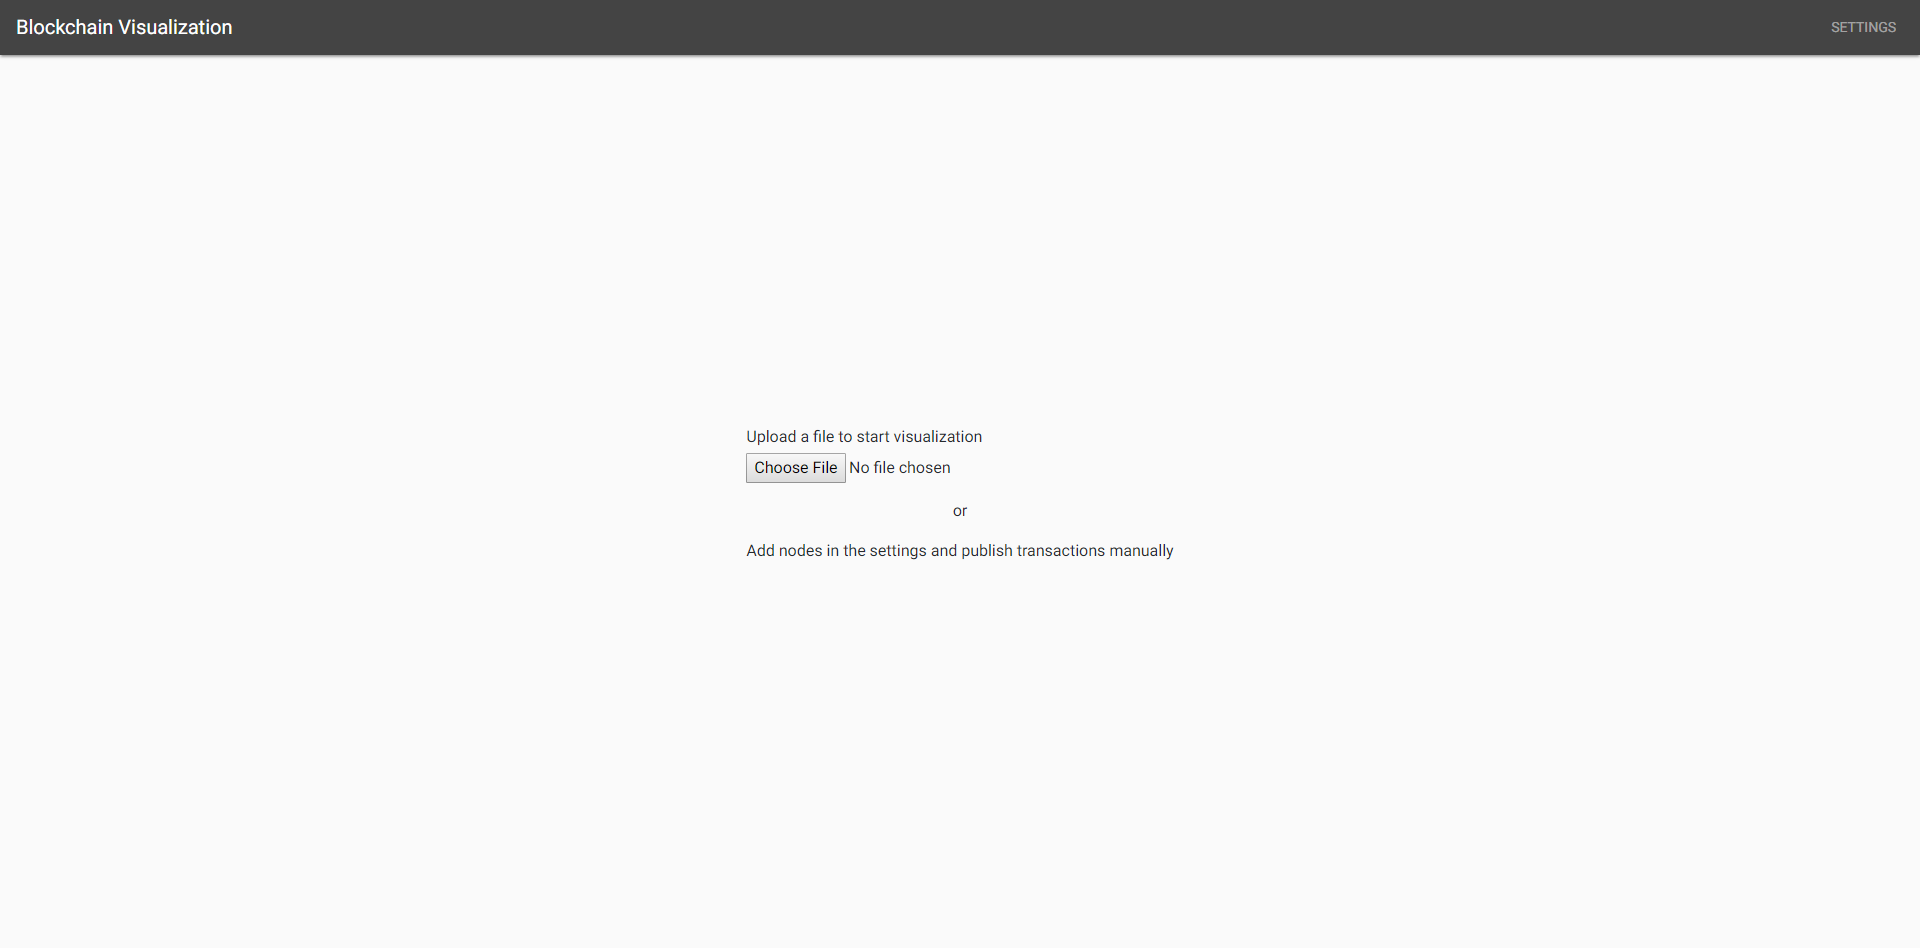
\includegraphics[width=\textwidth]{application_start}
    \caption{Start of the Application.}
    \label{fig:start of the application}
\end{figure}

By clicking the top right button in the navigation bar, the user will be redirected to the settings page, as Figure \ref{fig:settings page} shows.

\begin{figure}[htb]
    \centering
    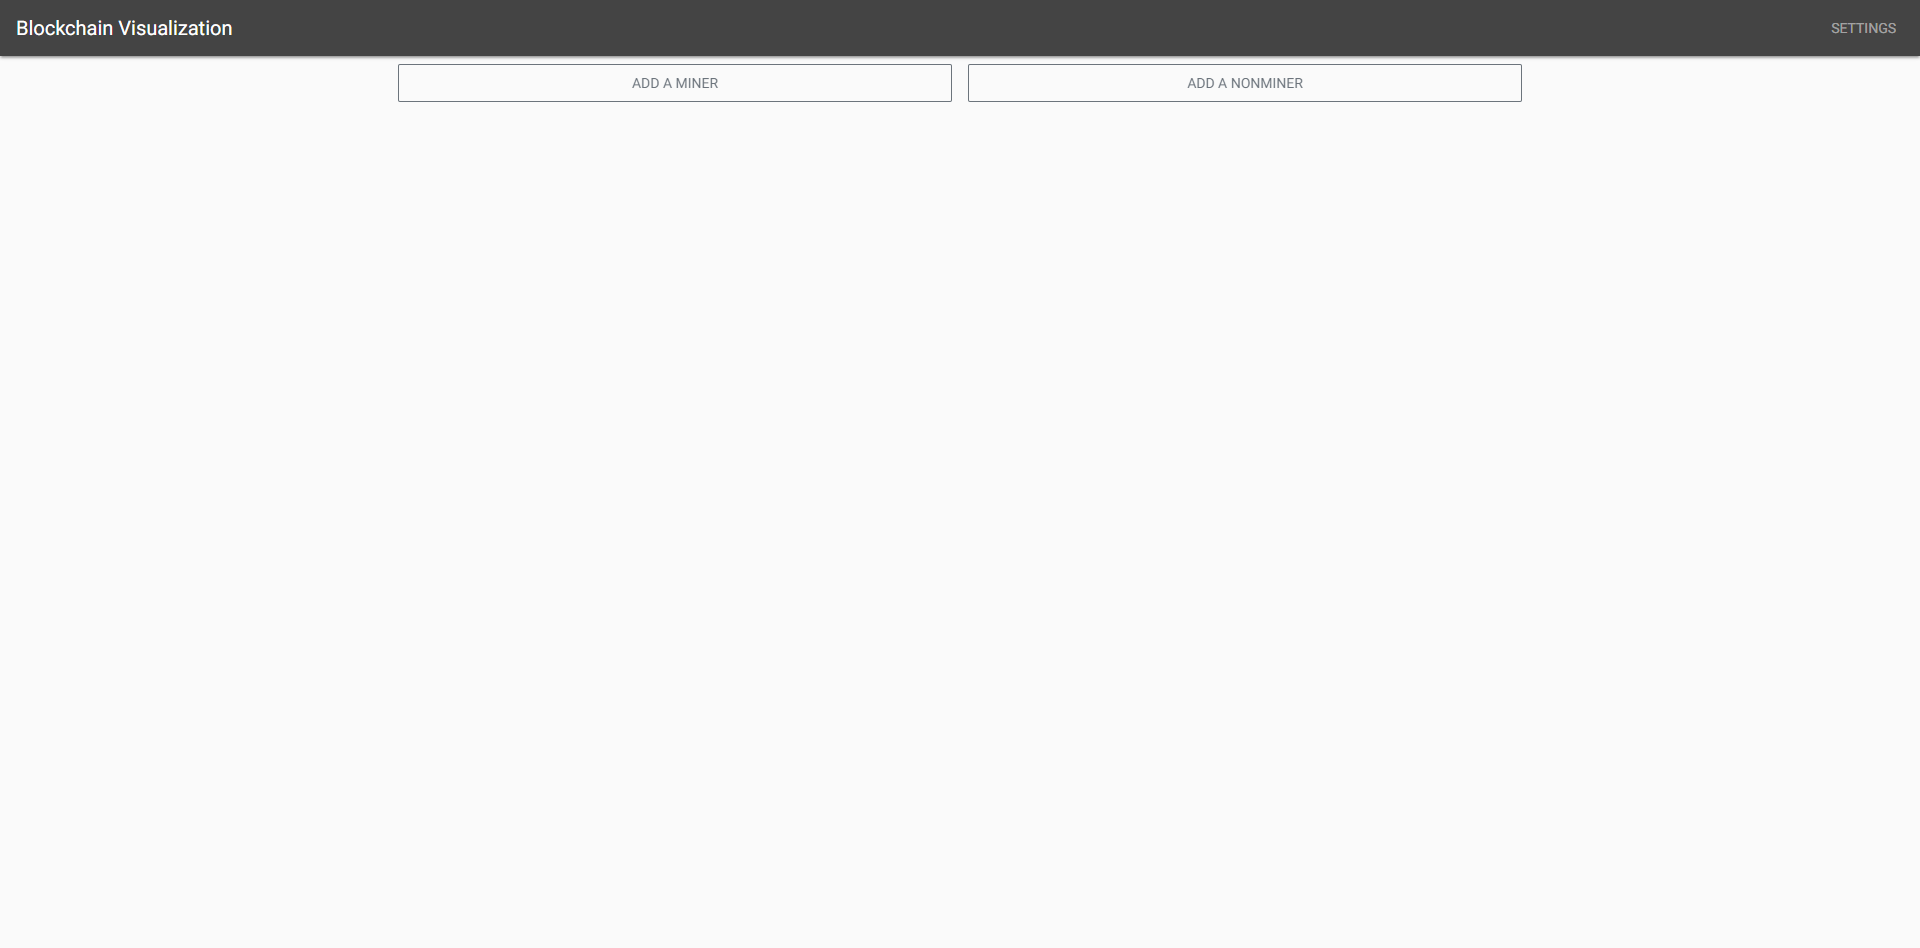
\includegraphics[width=\textwidth]{application_settings}
    \caption{Settings Page.}
    \label{fig:settings page}
\end{figure}

The settings page contains all the nodes that exist on the blockchain network. However, the blockchain system is empty currently, so the settings page is empty. To add a node, the user can click ``ADD A MINER'' button or ``ADD A NONMINER'' button. In this example, we add three miners and two nonminers.

\begin{figure}[htb]
    \centering
    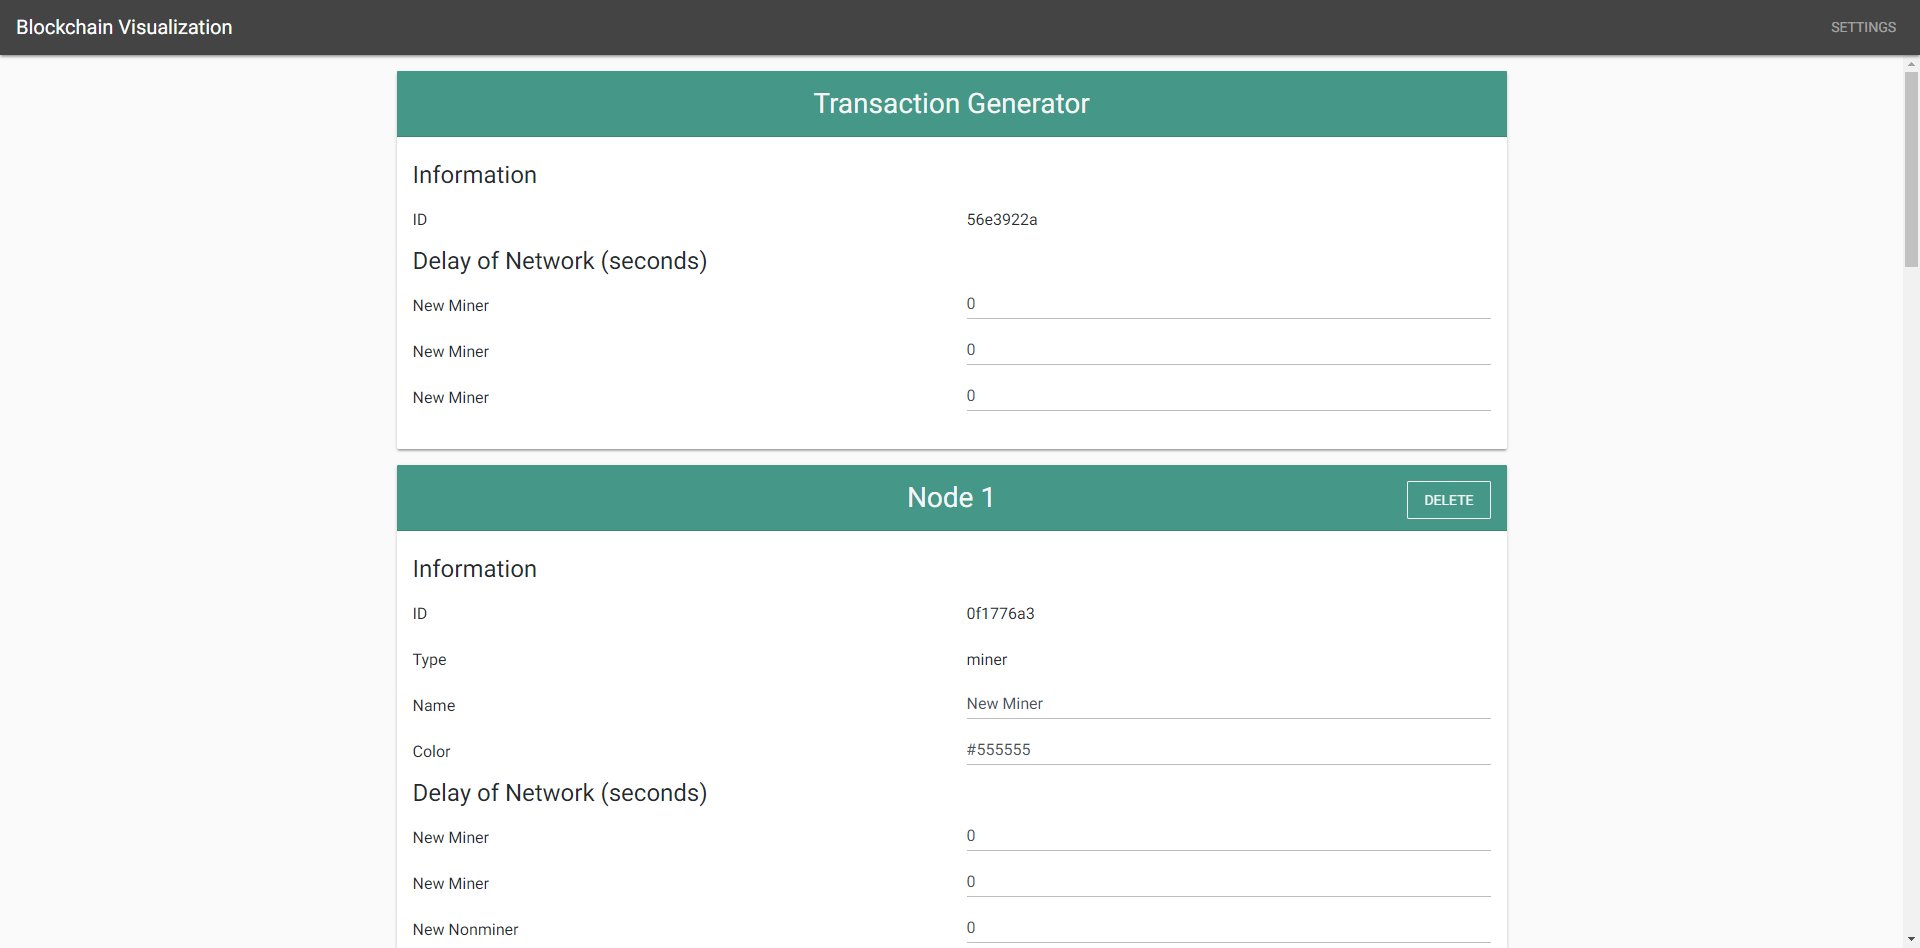
\includegraphics[width=\textwidth]{application_settings_tg}
    \caption{Settings of Transaction Generator.}
    \label{fig:settings of transaction generator}
\end{figure}

After creating nodes, the settings page contains three miners and two nonminers now. Additionally, the transaction generator is added to the blockchain system automatically. In Figure \ref{fig:settings of transaction generator}, the properties of the transaction generator are displayed in the most top block. The properties contain the ID and the network delay to its neighbors.

By scrolling down the settings page, the miners that exist in the blockchain system are displayed first. The parameters of the miners can be divided into three parts, as Figure \ref{fig:settings of miner} shows.

\clearpage

\begin{figure}[htb]
    \centering
    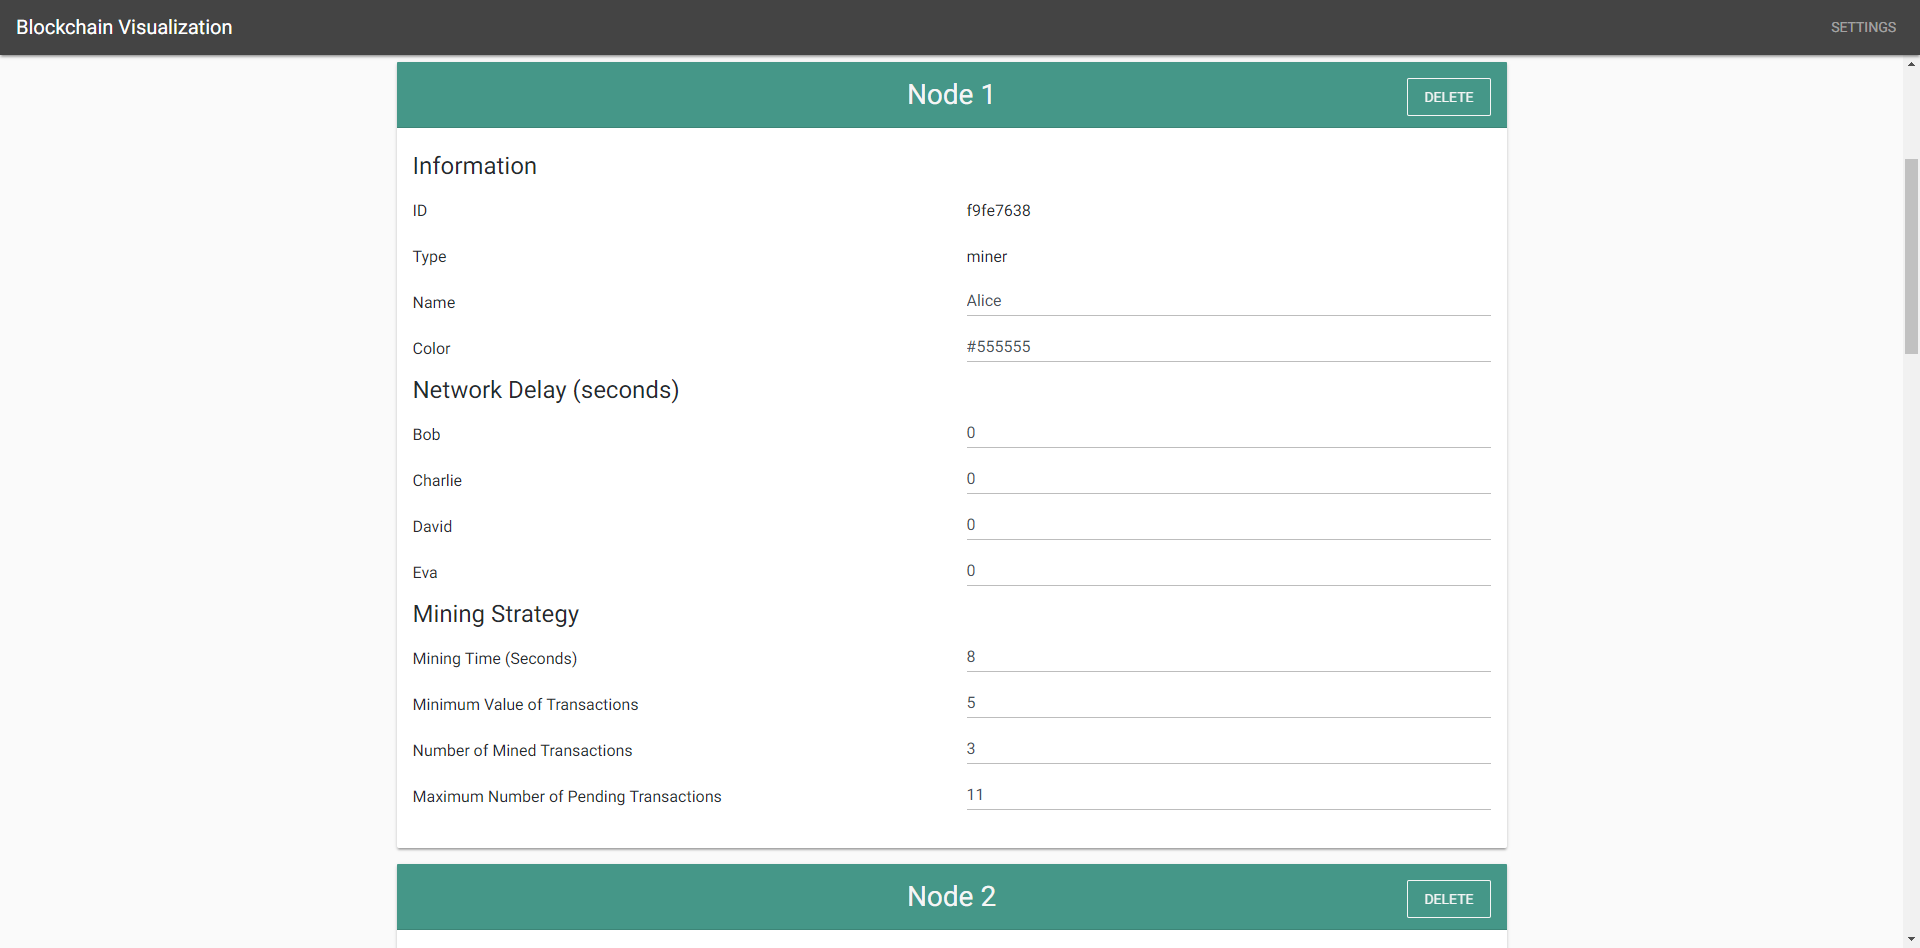
\includegraphics[width=\textwidth]{application_settings_m}
    \caption{Settings of Miner.}
    \label{fig:settings of miner}
\end{figure}

\begin{itemize}
    \item \textbf{Information} \\
        The properties of the miner, including the ID, the name, and the represented color.
    \item \textbf{Network Delay} \\
        It defines the periods of delay to the neighbors.
    \item \textbf{Mining Strategy} \\
        This part contains the four parameters that are used for the mining strategy.
\end{itemize}

\begin{figure}[htb]
    \centering
    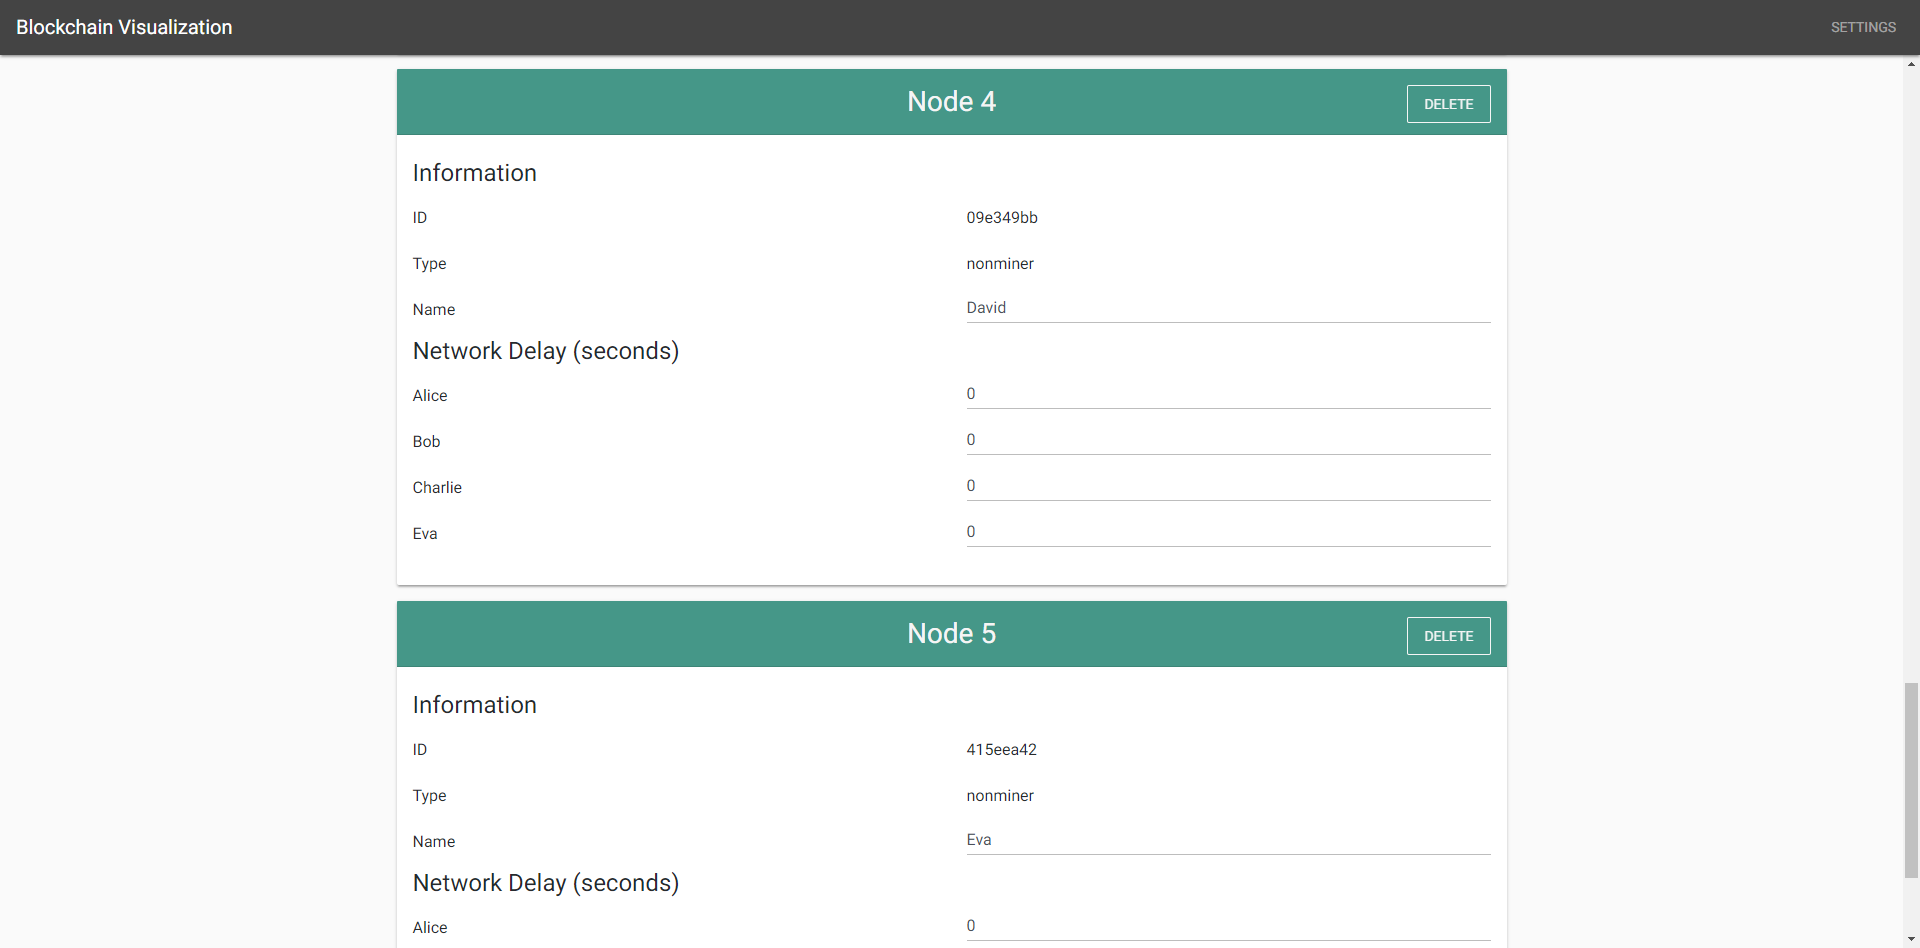
\includegraphics[width=\textwidth]{application_settings_nm}
    \caption{Settings of Nonminer.}
    \label{fig:settings of nonminer}
\end{figure}

The last part of the settings page is for the nonminers. Because nonminers do not mine a block by themselves, the represented color and the parameters of mining strategy are missing here, as Figure \ref{fig:settings of nonminer} shows.

The user can give miners and nonminers nicknames such as Alice, Bob, etc., to make the relationship between the nodes more understandable. The nicknames may not be unique in the blockchain system for the reason that the nodes are recognized by their unique IDs. Moreover, the parameters are updated automatically while the user is typing. All the parameters are generated randomly at first, so it is better to check and set each parameter manually.

In this example, we set Alice (red color), Bob (blue color), and Charlie (green color) as miners, and David and Eva as nonminers. For the mining strategy, we set the following three parameters to the same number for all miners.

\begin{itemize}
    \item Mining Time (Seconds): 1
    \item Number of Mined Transactions: 1
    \item Maximum Number of Pending Transactions: 10
\end{itemize}

For the parameters of \textit{minimum value of transactions}, we set 1 for Alice, 5 for Bob, and 9 for Charlie. Therefore, Alice is expected to mine blocks faster than Bob and Charlie. For the network delay, we set all the parameters to 1 second.

\begin{figure}[htb]
    \centering
    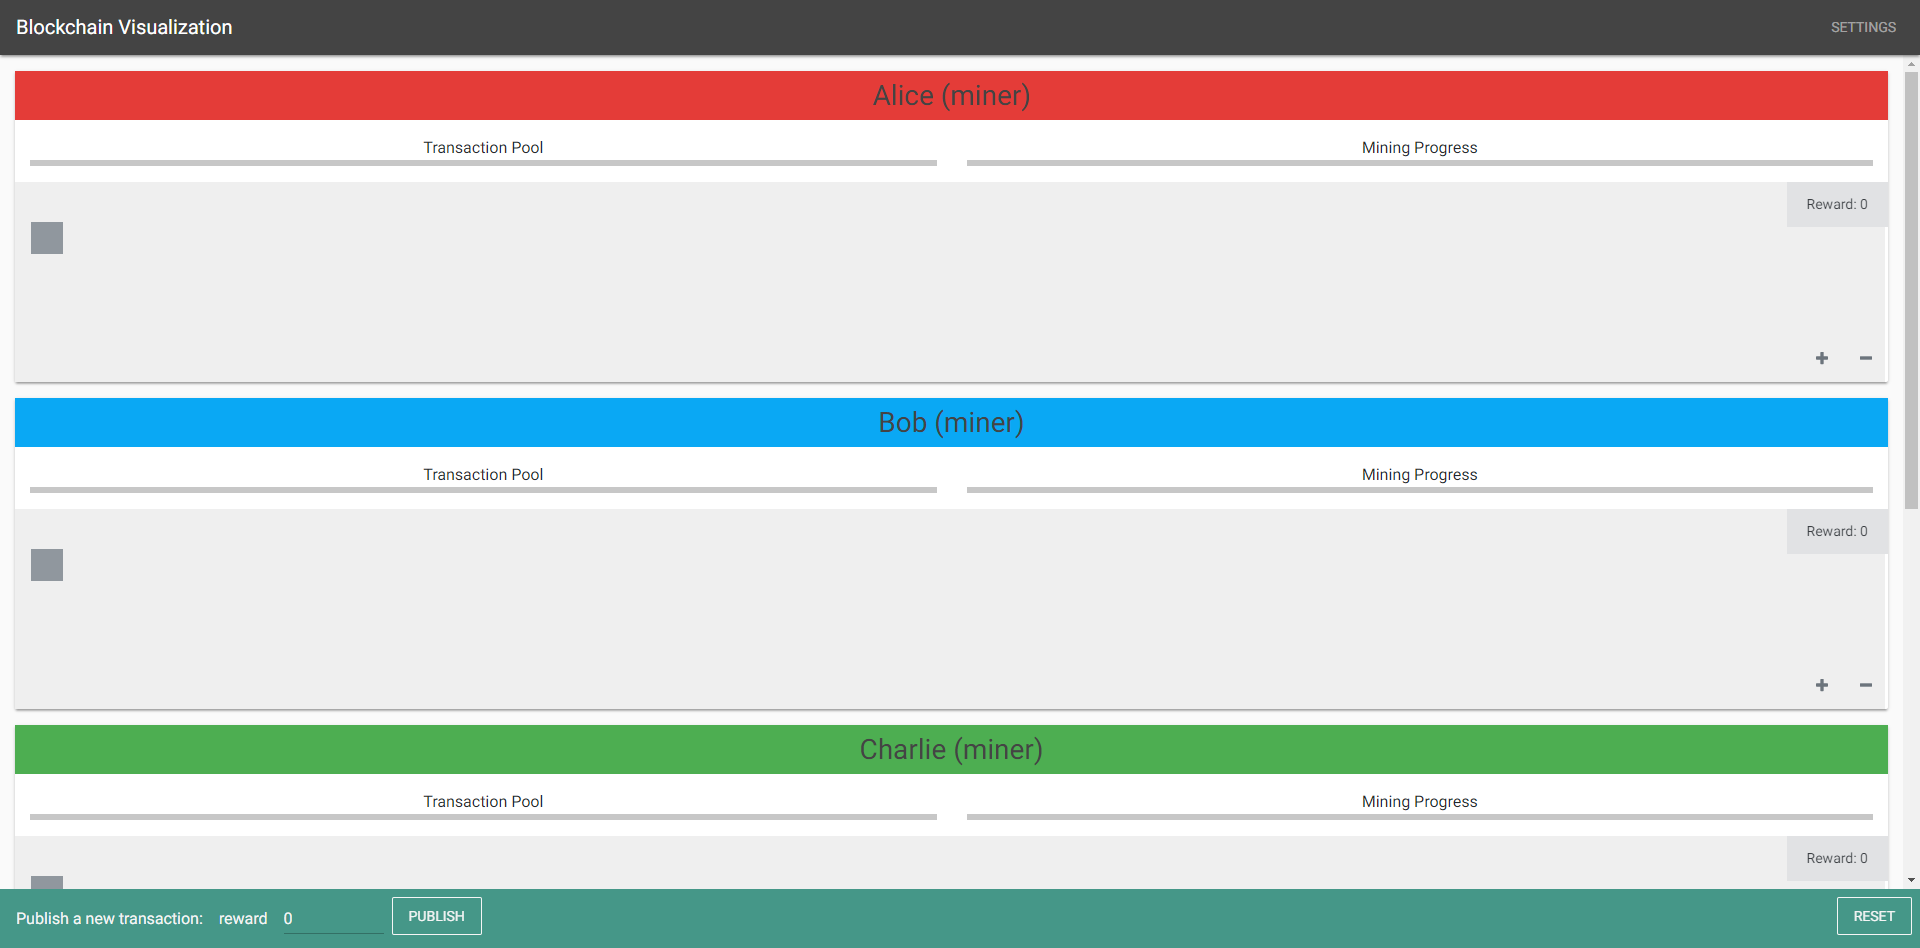
\includegraphics[width=\textwidth]{application_index}
    \caption{Initial status.}
    \label{fig:initial status}
\end{figure}

After finishing the configuration, the user can see the initial status of the blockchain system like Figure \ref{fig:initial status}. Each row represents the visualization of a miner or nonminer. A miner has a colorful head and two progress bars which display the status of the transaction pool and the mining activity. At the bottom of each row, it is the main area for visualizing the blockchain data structure. In the beginning, the grey block represents the genesis block.

\begin{figure}[htb]
    \centering
    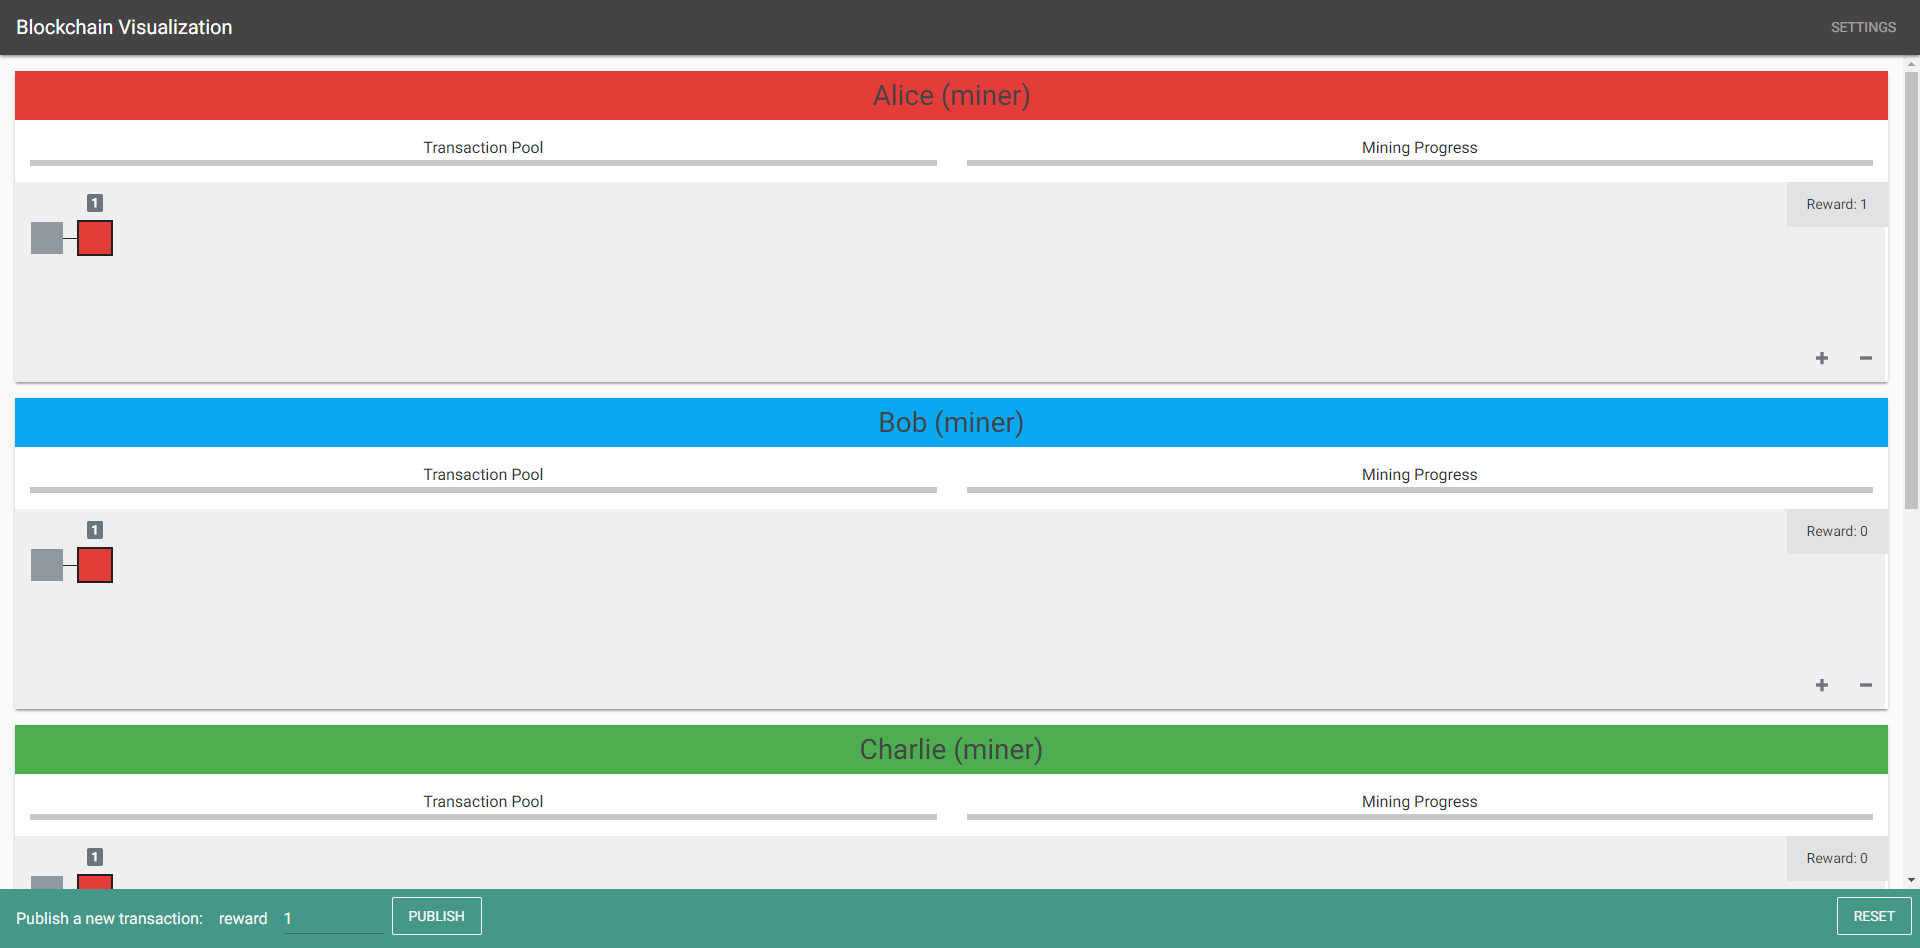
\includegraphics[width=\textwidth]{application_demo1}
    \caption{Alice mined a block.}
    \label{fig:alice mined a block}
\end{figure}

The user can publish a transaction at the bottom area of the screen. By entering a number of the reward, a transaction will be generated by the transaction generator and published. In the first step, we publish a transaction which reward is 1. Hence, it is expected that only Alice will mine a block because the \textit{minimum value of the transactions} is 1 for Alice, and the necessary \textit{number of mined transactions} is also 1. The result is showed in Figure \ref{fig:alice mined a block}. Moreover, now Alice's total reward is 1 because she added a block to the longest blockchain successfully.

\begin{figure}[htb]
    \centering
    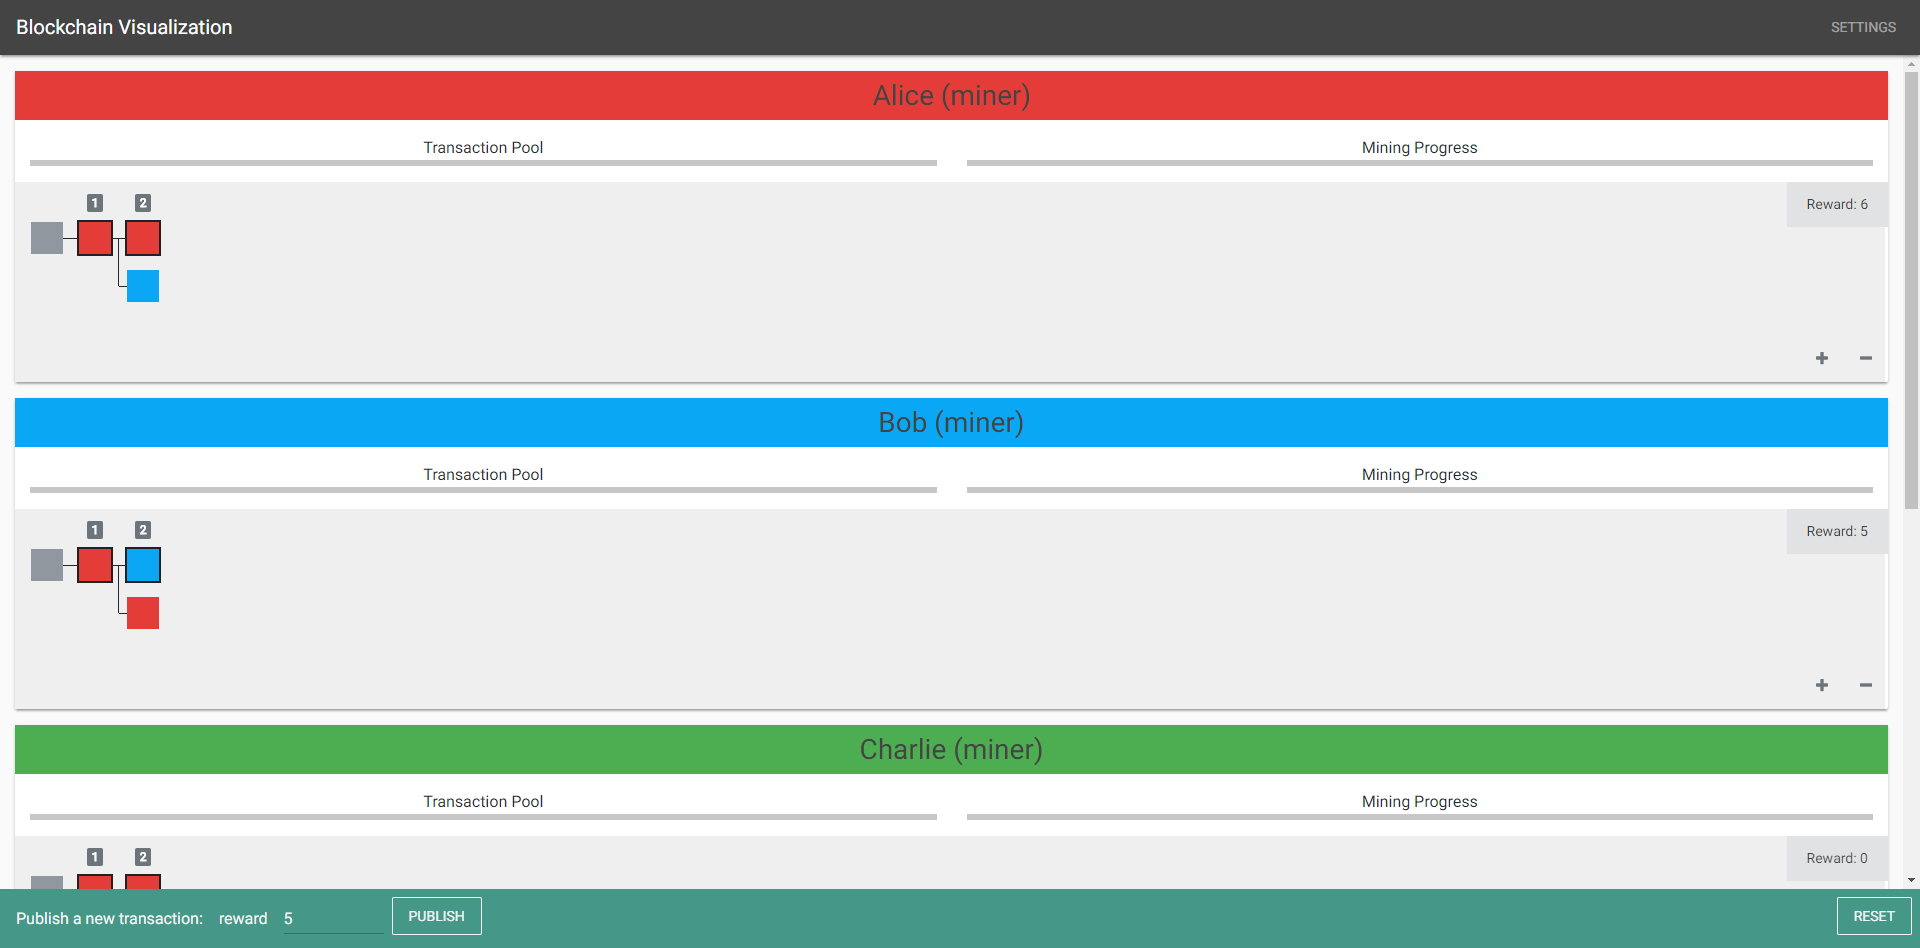
\includegraphics[width=\textwidth]{application_demo2}
    \caption{Alice and Bob mined a block simultaneously.}
    \label{fig:alice and bob mined a block simultaneously}
\end{figure}

Figure \ref{fig:alice and bob mined a block simultaneously} demonstrates that Alice and Bob competed with each other by adding a block at the same time. Because we published a transaction with reward of 5, Alice and Bob both decided to mine a block according to their mining strategies, i.e, the reward of the transaction is not less than their \textit{minimum value of the transactions}. As a result, the fork happened for the reason of simultaneous mining activities.

\begin{figure}[htb]
    \centering
    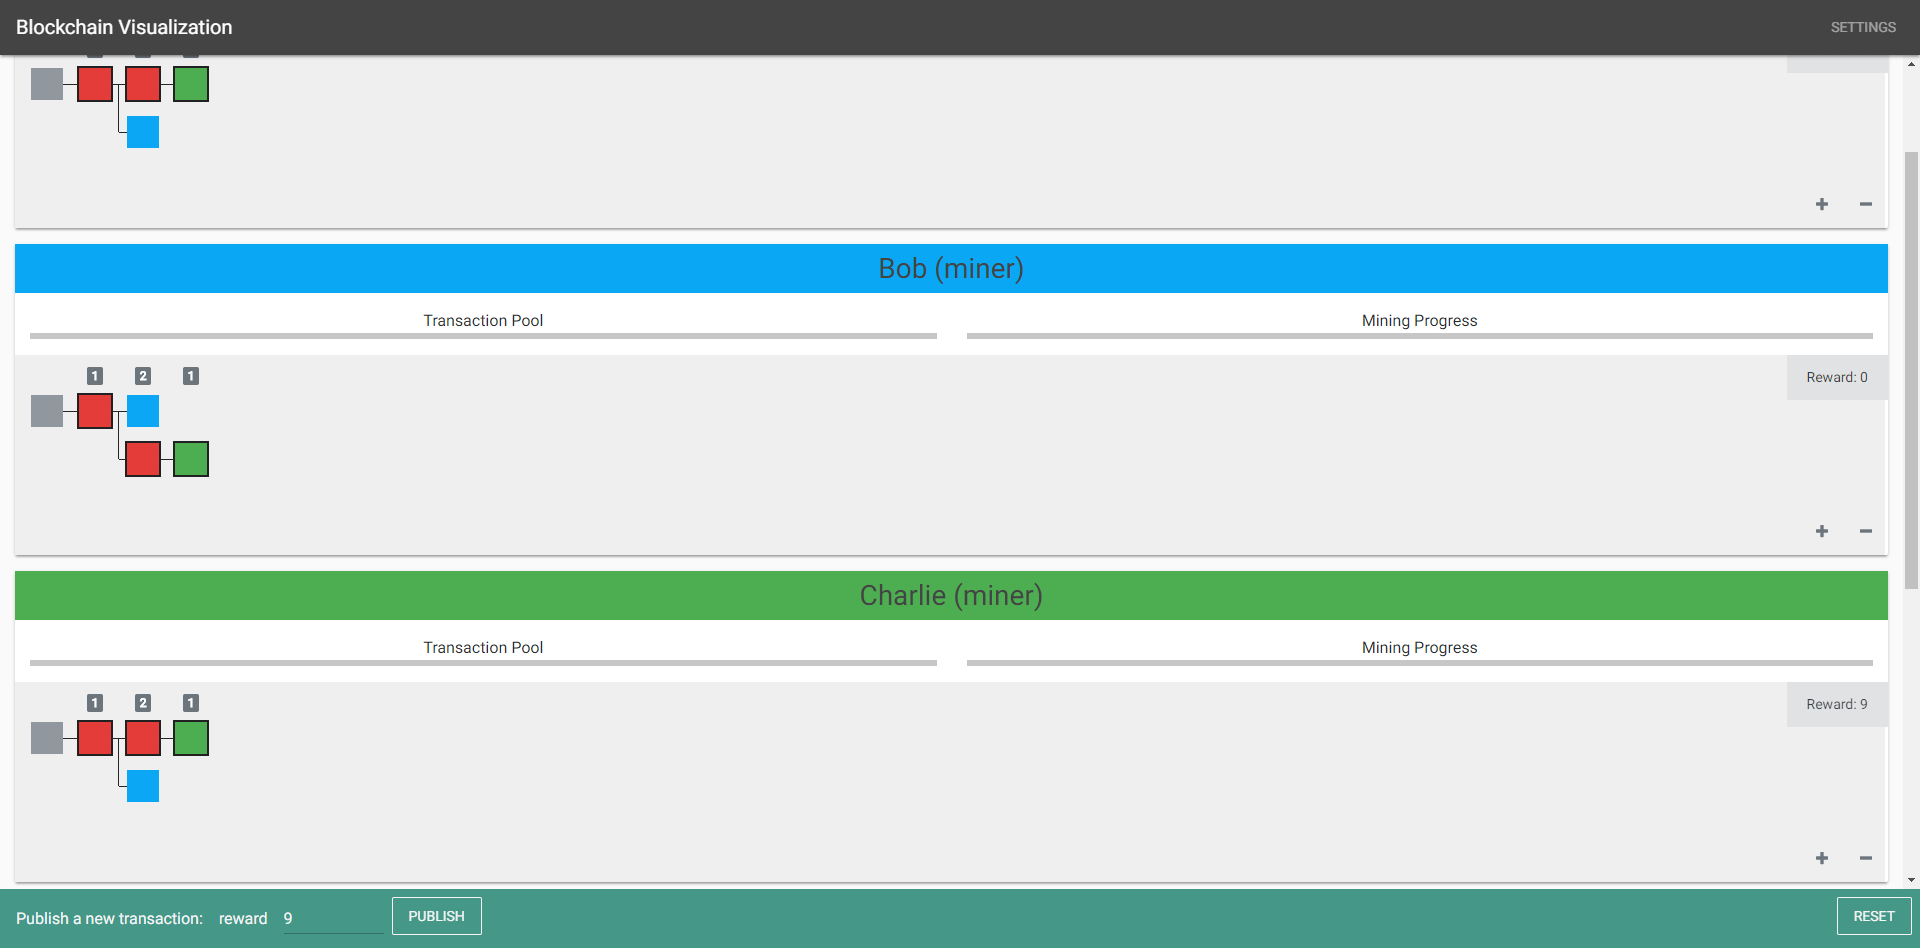
\includegraphics[width=\textwidth]{application_demo3}
    \caption{Charlie mined a block.}
    \label{fig:charlie mined a block}
\end{figure}

In the next step, Figure \ref{fig:charlie mined a block} shows the influence of the mining strategy to the mining processes. We changed the parameters of the mining strategy at first. Thus, Alice's and Bob's parameters of \textit{number of mined transactions} were both changed to 2. After that, a transaction with reward of 9 was published. The result was that Charlie mined a block for the reason that it satisfied Charlie's mining strategy, i.e, the \textit{number of mined transactions} is only 1 for Charlie. On the other hand, Alice and Bob did not mine a block because of the insufficient number of transactions.

\begin{figure}[htb]
    \centering
    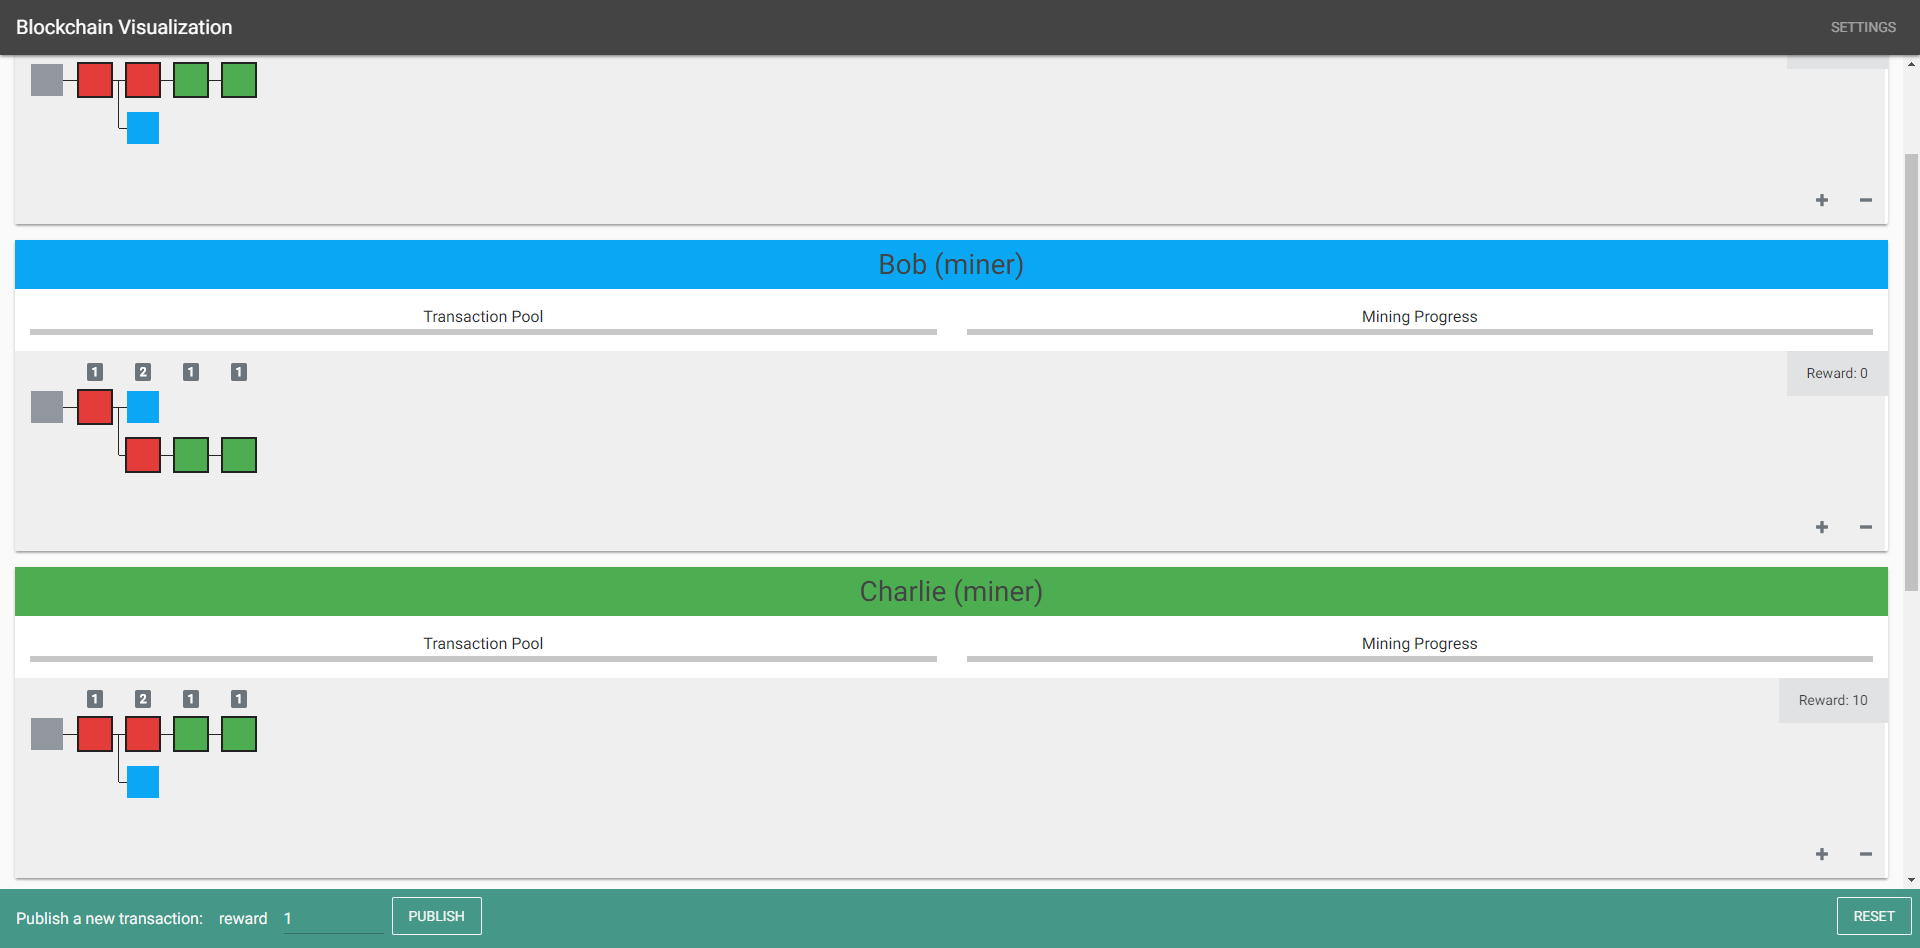
\includegraphics[width=\textwidth]{application_demo4}
    \caption{Charlie mined another block.}
    \label{fig:charlie mined another block}
\end{figure}

Figure \ref{fig:charlie mined another block} shows the process of selecting candidate transactions. We published a transaction with reward of 1. The result was that Charlie mined a block after about 8 seconds due to the process of selecting candidate transactions. Normally, a miner starts to select candidate transactions in every second, and the privileges of transactions that are not selected were added by 1 each time. Consequently, the value of the published transaction was becoming 9 after 8 seconds, and it satisfied Charlie's mining strategy, i.e., the \textit{minimum value of the transactions}.

\begin{figure}[htb]
    \centering
    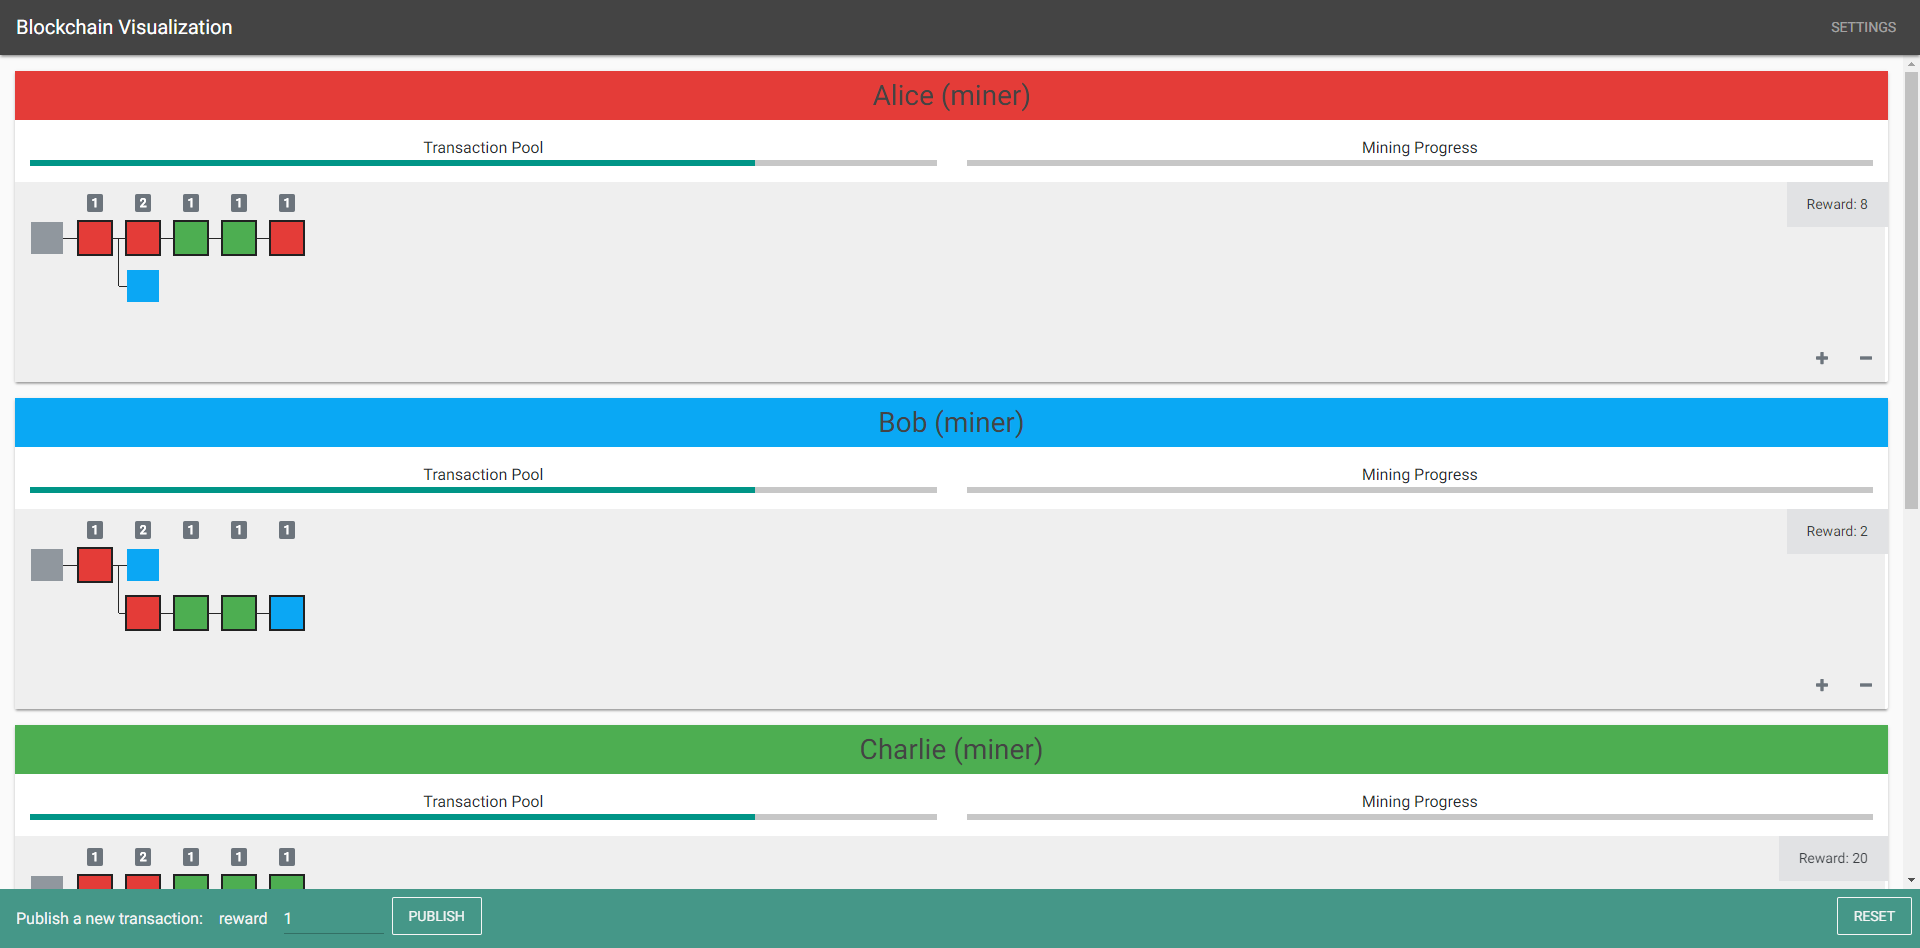
\includegraphics[width=\textwidth]{application_demo5}
    \caption{Overflow of transaction pools.}
    \label{fig:overflow of transaction pools}
\end{figure}

Finally, Figure \ref{fig:overflow of transaction pools} shows the overflow of the transaction pools. First, the parameters of \textit{minimum value of the transactions} were all set to 15 for the three miners, and then we published multiple transactions with the reward of 1. Because of a large number of transactions with low reward is published, the transaction pools became full in a short time, and it was displayed in the progress bars for transaction pools. As mentioned in the mining algorithm, all the three miners are forced to mine a block due to the overflow of the transaction pools, i.e., the number of pending transactions is larger than 10 in this example. The result can be checked in Figure \ref{fig:alice, bob, and charlie were forced to mine}, and it is the same as the expectation that all miners mine blocks simultaneously.

\begin{figure}[htb]
    \centering
    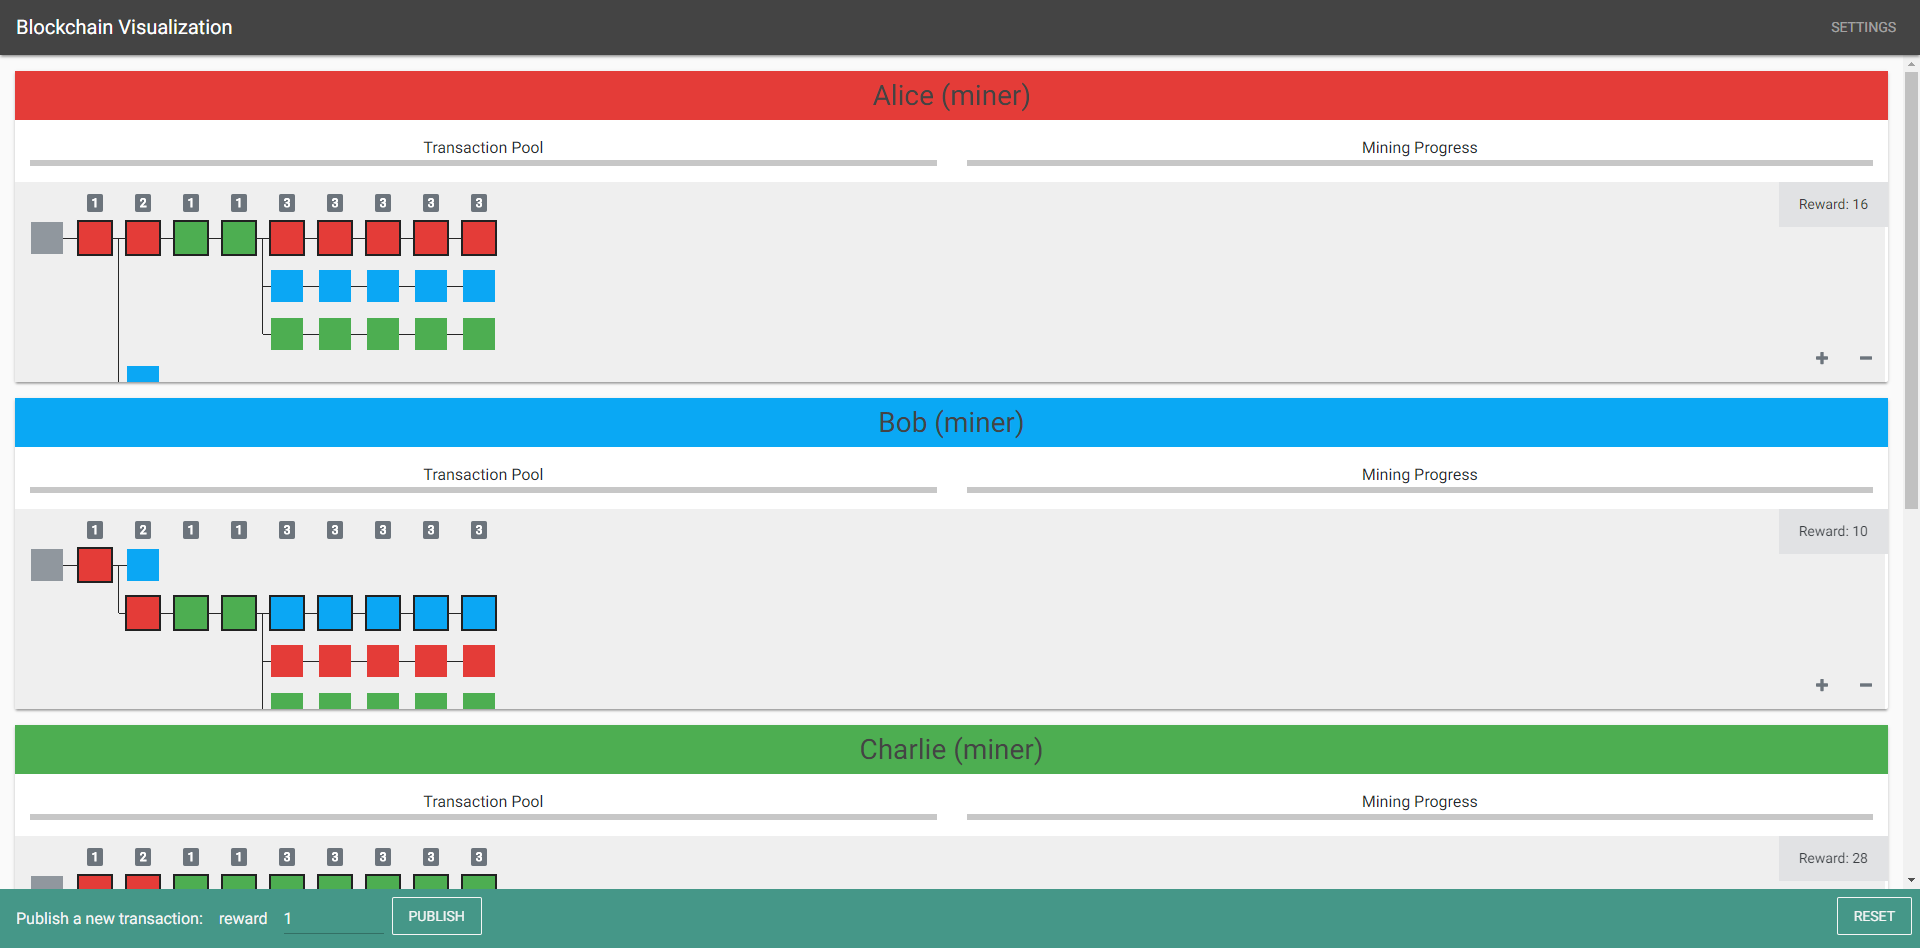
\includegraphics[width=\textwidth]{application_demo6}
    \caption{Alice, Bob, and Charlie were forced to mine.}
    \label{fig:alice, bob, and charlie were forced to mine}
\end{figure}

\clearpage

During the mining processes, the following auxiliary information in the visualization is also helpful and dynamic.

\begin{itemize}
    \item \textbf{Progress bars for the transaction pool} \\
        It displays the level of capacity of the transaction pool.
    \item \textbf{Progress bars for the mining status} \\
        It presents the mining activities in real-time, i.e., how much time is remaining for solving a puzzle.
    \item \textbf{Number of total reward} \\
        It displays the calculation of the total reward that belongs to the miner.
    \item \textbf{Number of forks} \\
        On the top of each fork, there is a number that represents the number of forks.
\end{itemize}

Additionally, the user can drag the visualization area to move the blockchain data structure, and zoom in and out by clicking the plus and minus buttons on the bottom right side.

\section{Configuration Files}

To replay the same visualization of blockchain processes, we can define the configuration of the blockchain system in a file and upload it to the application as in Figure \ref{fig:start of the application}. The configuration file is composed of the following three parts.

\begin{itemize}
    \item the properties and the parameters of the mining strategy of nodes
    \item the network delay between each node
    \item the transactions that will be published through the network
\end{itemize}

We provide a sample configuration file in Listing \ref{lst:sample of configuration file}. The file is in JSON format, and the file is used to initialize the blockchain system in the beginning.

First, for nodes, it is important to define a unique transaction generator at the beginning of the file, and then it is followed by miners and nonminers. The required properties for the transaction generator, miners, and nonminers are provided as the following.

\clearpage

\begin{enumerate}
    \item \textbf{Transaction Generator}
        \begin{itemize}
            \item id
            \item type
        \end{itemize}
    \item \textbf{Miner}
        \begin{itemize}
            \item id
            \item type
            \item color
            \item name
            \item miningTime
            \item minValue
            \item mineNumber
            \item maxPending
        \end{itemize}
    \item \textbf{Nonminer}
        \begin{itemize}
            \item id
            \item type
            \item name
        \end{itemize}
\end{enumerate}

Thd \textit{id} of nodes can be a string with arbitrary length, and here we use 8 characters and digits to represent the identifier. The \textit{type} distinguishes different nodes, and the valid values are \textit{generator}, \textit{miner}, and \textit{nonminer}. The \textit{name} of miners and nonminers are nicknames for them. Miners also have unique \textit{colors} to differentiate blocks in the visualization. The parameters of \textit{miningTime}, \textit{minValue}, \textit{mineNumber}, and \textit{maxPending} are from the mining strategy, which are \textit{mining time}, \textit{minimum value of transactions}, \textit{number of mined transactions}, \textit{minimum number of pending transactions} respectively.

The second part of the configuration file is a list of delay between each node. Each node has a block that begins with the \textit{id}, and then it is followed by a list of the neighbors and the amount of delay. As mentioned before, the transaction generator only has miners as neighbors, while miners and nonminers connect with each other. Moreover, the transaction generator is not in the neighbors of miners and nonminers because it is meaningless to send blocks to the transaction generator.

In the last part, it contains a list of transactions with the number of reward and the delay after the starting of the blockchain system, i.e., we can arrange the transactions to be published in a sequence.

\clearpage

\begin{lstlisting}[caption={Sample of Configuration File}, label={lst:sample of configuration file}]
{
    "nodes": [
        // transaction generator
        {
            "id": "6f71279b",
            "type": "generator"
        },
        // miner (Alice)
        {
            "id": "f1e50b4f",
            "type": "miner",
            "color": "#e53935",
            "name": "Alice",
            "miningTime": 1,
            "minValue": 1,
            "mineNumber": 1,
            "maxPending": 10
        },
        // nonminer (David)
        {
            "id": "480b945f",
            "type": "nonminer",
            "name": "David"
        },
    ],
    "delays": [
        // transaction generator
        {
            "id": "6f71279b",
            "neighbors": [
                {
                    "id": "f1e50b4f",
                    "seconds": 1
                }
            ]
        },
        // miner (Alice)
        {
            "id": "f1e50b4f",
            "neighbors": [
                {
                {
                    "id": "480b945f",
                    "seconds": 1
                }
            ]
        },
        // nonminer (David)
        {
            "id": "480b945f",
            "neighbors": [
                {
                    "id": "f1e50b4f",
                    "seconds": 1
                }
            ]
        }
    ],
    "transactions": [
        {
            "reward": 2,
            "delay": 0
        }
    ]
}
\end{lstlisting}

\chapter{Scenarios}
In this chapter, we explore three different scenarios that can be achieved by the visualization application. The first demonstrates the influences of the mining strategy, and the second scenario also adds the influences of network delay to the visualization. In addition, the presentation of orphaned blocks and forks proves that the visualization application handles the mining processes correctly. In the last scenario, we explore the limitation of the visualization application.

\section{A Fast Miner}

In the first scenario, there is a fast miner who mines blocks much quicker than the other miners due to the mining strategy. With the low network delay, the fast miner can publish the blocks quickly. Therefore, none of the other miners can compete with the fast miner, i.e., only the fast miner can add blocks to the blockchain.

In this experiment, there are three miners, Alice (red color), Bob (blue color), and Charlie (green color), who compete with each other in the blockchain system. The configuration of this experiment is provided in Configuration File \ref{lst:scenario 1}.

\begin{lstlisting}[caption={Scenario 1}, label={lst:scenario 1}]
{
    "nodes": [
        // transaction generator
        {
            "id": "6f71279b",
            "type": "generator"
        },
        // miner (Alice)
        {
            "id": "f1e50b4f",
            "type": "miner",
            "color": "#e53935",
            "name": "Alice",
            "miningTime": 1,
            "minValue": 1,
            "mineNumber": 1,
            "maxPending": 10
        },
        // miner (Bob)
        {
            "id": "2d30b6fd",
            "type": "miner",
            "color": "#03a9f4",
            "name": "Bob",
            "miningTime": 5,
            "minValue": 4,
            "mineNumber": 3,
            "maxPending": 10
        },
        // miner (Charlie)
        {
            "id": "a6b877ab",
            "type": "miner",
            "color": "#4caf50",
            "name": "Charlie",
            "miningTime": 6,
            "minValue": 7,
            "mineNumber": 2,
            "maxPending": 10
        }
    ],
    "delays": [
        // transaction generator
        {
            "id": "6f71279b",
            "neighbors": [
                {
                    "id": "f1e50b4f",
                    "seconds": 1
                },
                {
                    "id": "2d30b6fd",
                    "seconds": 1
                },
                {
                    "id": "a6b877ab",
                    "seconds": 1
                }
            ]
        },
        // miner (Alice)
        {
            "id": "f1e50b4f",
            "neighbors": [
                {
                    "id": "2d30b6fd",
                    "seconds": 1
                },
                {
                    "id": "a6b877ab",
                    "seconds": 1
                }
            ]
        },
        // miner (Bob)
        {
            "id": "2d30b6fd",
            "neighbors": [
                {
                    "id": "f1e50b4f",
                    "seconds": 1
                },
                {
                    "id": "a6b877ab",
                    "seconds": 1
                }
            ]
        },
        // miner (Charlie)
        {
            "id": "a6b877ab",
            "neighbors": [
                {
                    "id": "f1e50b4f",
                    "seconds": 1
                },
                {
                    "id": "2d30b6fd",
                    "seconds": 1
                }
            ]
        }
    ],
    "transactions": [
        {
            "reward": 2,
            "delay": 0
        },
        {
            "reward": 3,
            "delay": 1
        },
        {
            "reward": 9,
            "delay": 2
        },
        {
            "reward": 4,
            "delay": 3
        },
        {
            "reward": 7,
            "delay": 4
        },
        {
            "reward": 5,
            "delay": 5
        },
        {
            "reward": 1,
            "delay": 6
        },
        {
            "reward": 5,
            "delay": 7
        },
        {
            "reward": 3,
            "delay": 8
        },
        {
            "reward": 2,
            "delay": 9
        }
    ]
}
\end{lstlisting}

As the configuration file shows, Alice's mining strategy is the fastest because the parameters of \textit{Mining Time}, \textit{Minimum Value of Transactions}, and \textit{Fixed Number of Transactions in Blocks} are all set to 1. On the contrary, Bob's and Charlie's parameters are both higher than Alice's parameters. The parameters of network delay are all set to 1. Hence, the blockchain network is stable and fast and it only takes 1 second to publish the blocks to neighbors. For transactions, we defined a sequence of transactions which interval is 1 second.

\begin{figure}[htb]
    \centering
    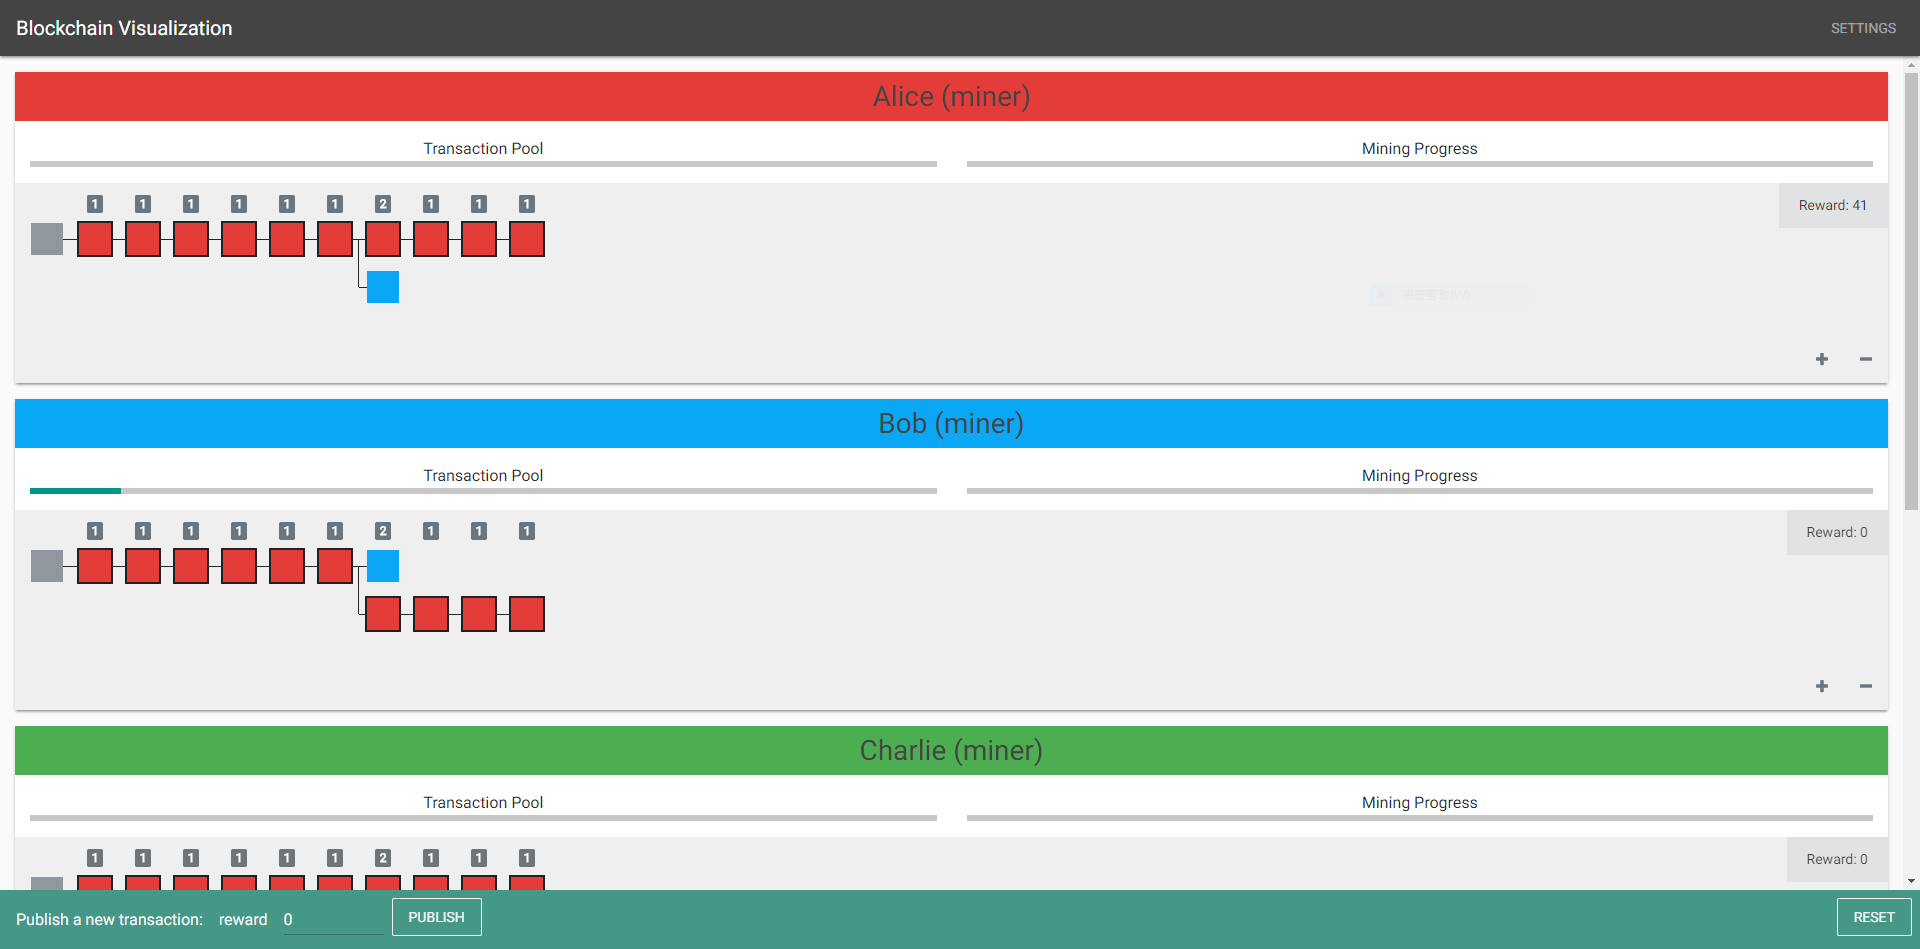
\includegraphics[width=\textwidth]{scenario_case1}
    \caption{Alice was a fast miner.}
    \label{fig:alice was a fast miner}
\end{figure}

In Figure \ref{fig:alice was a fast miner}, it demonstrates the results of the above configuration. Although some transactions have high number of reward, Alice still dominated the blockchain system because of her fast mining strategy. As a result, all of the 10 transactions were mined by Alice, even if Bob tried to mined a block at the seventh layer. 

In summary, this scenario shows the competition between the miners. As our expectation, the mining strategy with the lowest \textit{Mining Time}, \textit{Minimum Value of Transactions} and \textit{Fixed Number of Transactions in Blocks} is the fastest one. Additionally, it shows that the orphaned block were handled by the visualization application correctly, as the fast miner still worked on the correct blockchain data structure.

\section{Multiple Forks}

In the second scenario, there are three miners who have the similar computing power and mining strategies, and compete with each other for a long time. Because the spread of blocks suffers high delays, miners add their own blocks to the blockchain much more quickly than others do. Thus, each miner considers his/her own blockchain is the longest one, and the competition continues. Configuration File \ref{lst:scenario 2} is the configuration file for this scenario.

\begin{lstlisting}[caption={Scenario 2}, label={lst:scenario 2}]
{
    "nodes": [
        // transaction generator
        {
            "id": "6f71279b",
            "type": "generator"
        },
        // miner (Alice)
        {
            "id": "f1e50b4f",
            "type": "miner",
            "color": "#e53935",
            "name": "Alice",
            "miningTime": 1,
            "minValue": 1,
            "mineNumber": 1,
            "maxPending": 10
        },
        // miner (Bob)
        {
            "id": "2d30b6fd",
            "type": "miner",
            "color": "#03a9f4",
            "name": "Bob",
            "miningTime": 1,
            "minValue": 1,
            "mineNumber": 1,
            "maxPending": 10
        },
        // miner (Charlie)
        {
            "id": "a6b877ab",
            "type": "miner",
            "color": "#4caf50",
            "name": "Charlie",
            "miningTime": 1,
            "minValue": 1,
            "mineNumber": 1,
            "maxPending": 10
        }
    ],
    "delays": [
        // transaction generator
        {
            "id": "6f71279b",
            "neighbors": [{
                    "id": "f1e50b4f",
                    "seconds": 1
                },
                {
                    "id": "2d30b6fd",
                    "seconds": 1
                },
                {
                    "id": "a6b877ab",
                    "seconds": 1
                }
            ]
        },
        // miner (Alice)
        {
            "id": "f1e50b4f",
            "neighbors": [{
                    "id": "2d30b6fd",
                    "seconds": 3
                },
                {
                    "id": "a6b877ab",
                    "seconds": 3
                }
            ]
        },
        // miner (Bob)
        {
            "id": "2d30b6fd",
            "neighbors": [{
                    "id": "f1e50b4f",
                    "seconds": 3
                },
                {
                    "id": "a6b877ab",
                    "seconds": 3
                }
            ]
        },
        // miner (Charlie)
        {
            "id": "a6b877ab",
            "neighbors": [{
                    "id": "f1e50b4f",
                    "seconds": 3
                },
                {
                    "id": "2d30b6fd",
                    "seconds": 3
                }
            ]
        }
    ],
    "transactions": [
        {
            "reward": 2,
            "delay": 0
        },
        {
            "reward": 3,
            "delay": 1
        },
        {
            "reward": 9,
            "delay": 2
        },
        {
            "reward": 4,
            "delay": 3
        },
        {
            "reward": 7,
            "delay": 4
        },
        {
            "reward": 5,
            "delay": 5
        },
        {
            "reward": 1,
            "delay": 6
        },
        {
            "reward": 5,
            "delay": 7
        },
        {
            "reward": 3,
            "delay": 8
        },
        {
            "reward": 2,
            "delay": 9
        }
    ]
}
\end{lstlisting}

In the configuration file, Alice's, Bob's and Charlie's parameters of the mining strategy are set to the same value. Therefore, it is expected that the three miners will always mine at the same time. The parameters of the network delay are higher than the parameters of \textit{Mining Time} to simulate the bad network conditions between three miners. The sequence of transactions are the same as Configuration File \ref{lst:scenario 1}.

\begin{figure}[htb]
    \centering
    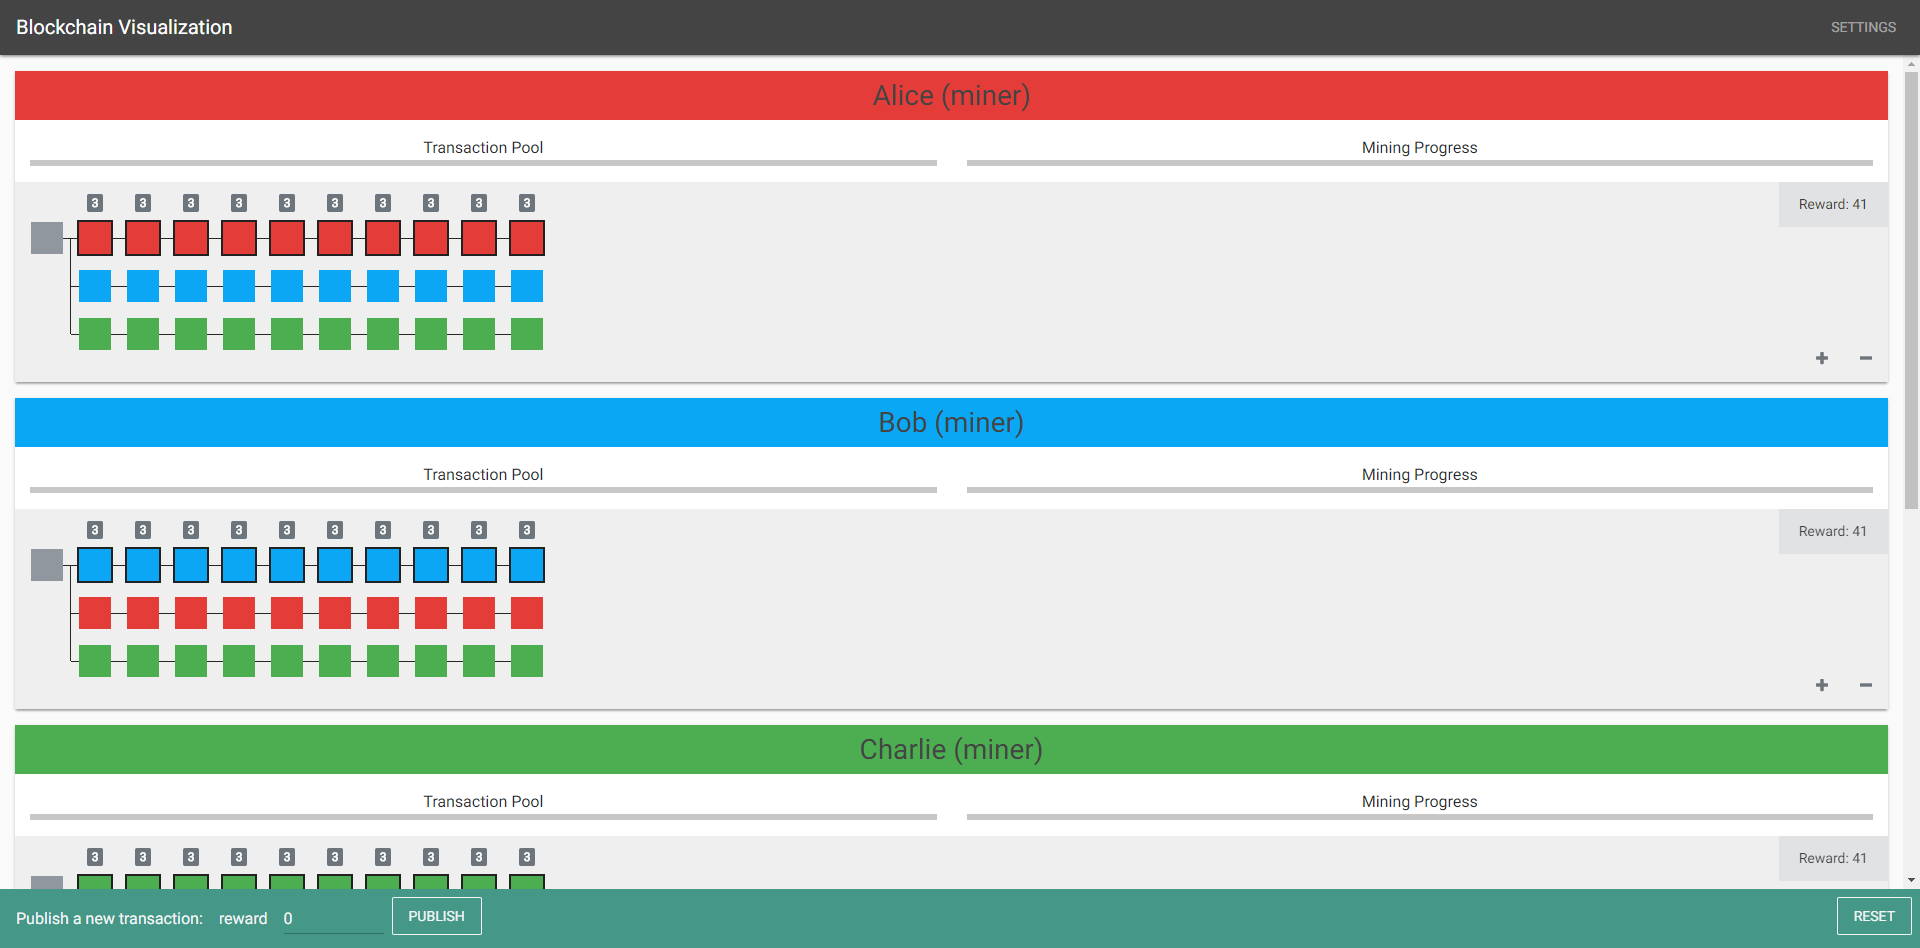
\includegraphics[width=\textwidth]{scenario_case2}
    \caption{Alice, Bob, and Charlie competed with each other.}
    \label{fig:alice, bob, and charlie competed with each other}
\end{figure}

In Figure \ref{fig:alice, bob, and charlie competed with each other}, Alice, Bob, and Charlie compete with each other for a long time because the duration of mining time is shorter than the duration of publishing blocks. The miners are divided into three groups which work on different blockchain data structures because every miner considered that their own blockchain is the longest. It can be checked that the mining processes visualized the mining processes according to the above description, as Figure \ref{fig:the mining processes of scenario 2} shows.

\begin{figure}[htb]
    \centering
    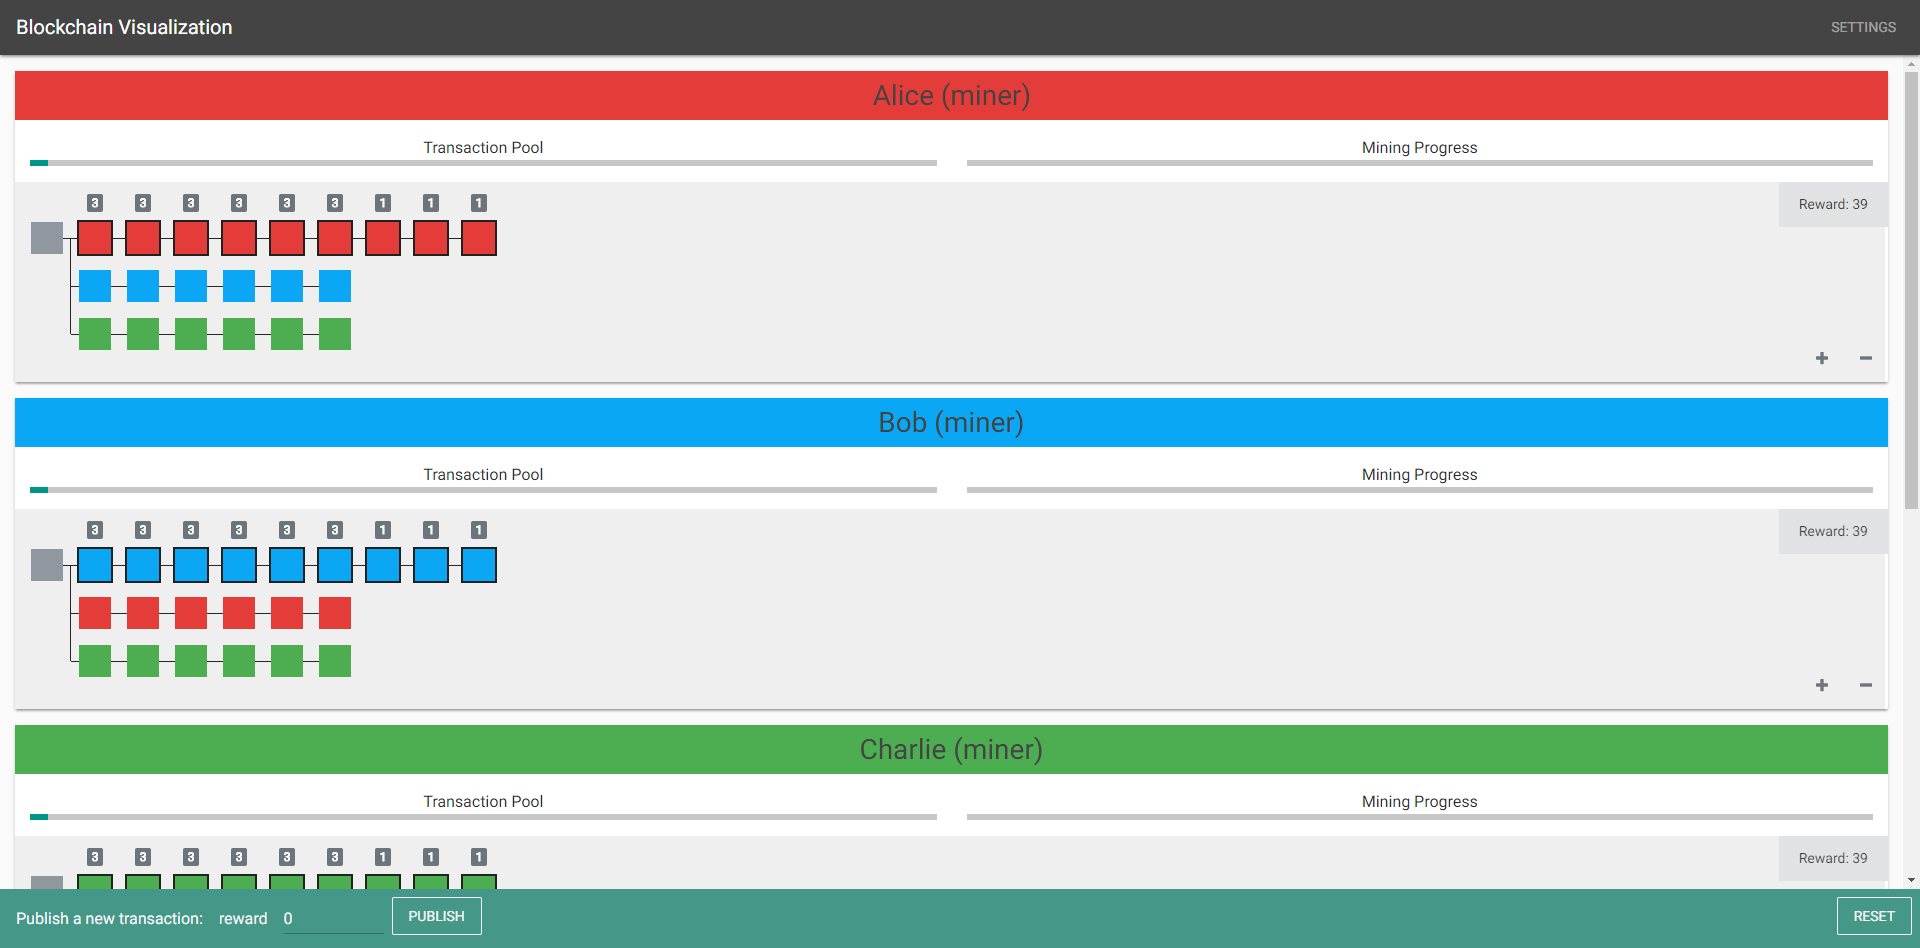
\includegraphics[width=\textwidth]{scenario_case2_2}
    \caption{The mining processes of scenario 2.}
    \label{fig:the mining processes of scenario 2}
\end{figure}

In conclusion, it demonstrates that the visualization application is able to handle the forks correctly. Furthermore, the mining processes are also correct. However, there is a weak point in the visualization application. The forks cannot be merged in the current implementation because the parameters of the mining strategy are fixed during the visualization. Thus, the scenario of multiple forks in the visualization represent the scenario of the hard forks in the real blockchain networks. It should be improved to handle the scenario of the soft forks in the future.

\section{Limitation of Nodes and Transactions}

Through experiments, we found that the maximum number of nodes that can be handled by the application is 15 because of the limitation of the visualization engine, i.e., the Three.js library. The visualization engine cannot created too much canvases due to the performance issue. Hence, the sum of the number of miners and nonminers is limited to 15. On the other hand, the number of transactions that can be handled should be unlimited. We tested it by publishing 100 transactions, and the application still operates correctly.



\chapter{Conclusion}
\section{Summary}

This thesis proposes the first trial to visualize the complex and dynamic mining processes in the blockchain system. The visualization is based on the simulation of the blockchain system which is powered by the multi-agent system. With the watchdog which monitors the data in the blockchain system, the visualizer can update the visualization in real-time after it receives the data from the watchdog. The visualization of blockchain processes clearly indicates the mining activities step by step. 

The visualization application helps researchers to conduct experiments and focus on the mining activities which are influenced by the network delay and the mining strategy in the blockchain system. By providing a configuration file which defines all the properties and parameters in the blockchain system, the same mining processes can be replayed by the visualization application. With the discussions of the scenarios, it proves the potential applications of the visualization application.

\section{Future Work}

In the future, we plan to do the following improvements to the visualization application.

\begin{itemize}
    \item \textbf{Add different consensus protocols} \\
        The consensus protocol can be extended to include other algorithms, such as proof-of-stake. Therefore, researchers can switch between different consensus protocols to compare different mining behaviors.
    \item \textbf{Add malicious nodes} \\
        To simulate the attacks on the blockchain system, malicious nodes should be included in the application. Thus, we need to improve the algorithm of consensus protocols to validate and detect malicious nodes.
    \item \textbf{Dynamic nodes} \\
        In a peer-to-peer network, nodes can jump in and out at any time. Ensuring the dynamic creations and deletions while the visualization is running could be a good feature.
    \item \textbf{Merge of forks} \\
        To solve the merge problem in the second scenario, the naive solution is to provide a randomness to the parameters in the blockchain system. For example, the duration of mining time should be randomness between a range because solving a puzzle cannot be predicted in the real blockchain system.
    \item \textbf{Confirmation of blocks} \\
        The longest blockchain sometimes changes in the visualization. It can be improved to implement the confirmation of blocks. For example, a block is confirmed if it is 6 blocks deep and on the longest blockchain in Bitcoin.
\end{itemize}


\bibliographystyle{IEEEtran}
\bibliography{references}

\appendix
\chapter{Source Codes}
The source codes are maintained under the following link:

\url{https://scm.fit.fraunhofer.de/scm/git/BlockchainVisualizer}

The repository is hosted by Department of Risk Management And Decision Support, Fraunhofer FIT. All rights are reserved.



\end{document}

